%%% -*-LaTeX-*-
%%% ====================================================================
%%% This is a sample top-level LaTeX-2e file for typesetting a thesis
%%% or dissertation at the University of Utah.  Most students find it
%%% convenient to start with a COPY of this file as a template, and
%%% then alter that copy to match their needs.
%%%
%%% There is an associated Unix Makefile that can be similarly
%%% customized, and then the only command ever needed to typeset the
%%% complete thesis is the single word "make".  Of course, during
%%% writing and typesetting, not all of the steps are needed, so
%%% often, one can just name a convenience target such as "make
%%% dvi-pass" or "make pdf-pass" to do just a single pass of LaTeX and
%%% BibTeX.
%%%
%%% There should be no, or very few, macro definitions in this file;
%%% any needed belong in a private style file, called mythesis.sty,
%%% and input below after all other packages.  The bulk of this file
%%% should just be command invocations, and any arguments that they
%%% need.
%%%
%%% We exploit the fact that TeX ignores spaces after command names to
%%% line up arguments for better readability.
%%%
%%% Each chapter should be a separate complete file, so that you can
%%% insert a command like \includeonly{chap_intro} before the first
%%% \include{chap_xxx} command to avoid typesetting all but the
%%% chapter that you are currently working on, to save time.
%%%
%%% Remember that occupants of job positions change jobs from time to
%%% time: YOU are responsible for ensuring correct names of all humans
%%% mentioned in this file!
%%%
%%% [16-Mar-2016]
%%% ====================================================================

\documentclass[11pt,Chicago]{uuthesis2e}

%%% Undefine two macros from uuthesis2e.cls that conflict with
%%% definitions in amsthm.sty that fail to check for prior definitions!
%%% NB: The amsthm package refines the LaTeX theorem environment,
%%% and the uuthesis-color-headings wraps that definition, so the
%%% amsthm package must be read first!
\let \proof    = \relax
\let \endproof = \relax
\usepackage {amsthm}

%%% ====================================================================
%%% Choose an alternate font family for the document if the TeX default
%%% of Computer Modern is not wanted:

\RequirePackage{times}

%%% ====================================================================
%%% Some miscellaneous Utah- and student-specific settings:
%%%
%%% Chapter is one level, section and subsection are the next two levels.

\fourlevels

%%% ====================================================================
%%% The remaining packages are required by this particular thesis,
%%% but other theses will almost certainly need different packages:
%%%
%%% WARNING: MANY \LaTeX{} packages change dimensions, glue, and/or
%%% formatting styles, and such changes are likely to conflict with
%%% University of Utah Thesis Office requirements.  Therefore, minimize
%%% the number of packages that you include!

\usepackage
{
    cite, 
    epsfig,
    epstopdf, 
    graphicx, 
    color, 
%    float,
    subfig,
    amssymb,
    xspace,
    tabularx,
    rotating,
    lscape,
    afterpage,
    url,
    listings,
    multirow,
    hhline,
    placeins
} 

\usepackage{amsmath}
\usepackage{algorithmic}
\renewcommand{\algorithmicrequire}{\textbf{Input:}}
\renewcommand{\algorithmicensure}{\textbf{Output:}}

\usepackage{polynom}
\usepackage{blkarray}
\usepackage{enumerate}

\usepackage[ruled]{./algorithm2e}

\newcommand{\ov}{\bar}
\newcommand{\xor}{\bigoplus}
\newcommand{\tab}{\xspace\ \ \ \ \xspace}
\newcommand{\ttab}{\xspace\ \ \xspace}

\newcommand{\eqntext}[1]{\text{\xspace\rm #1\xspace}}

\newcommand{\Fq}{{\mathbb{F}}_{q}}
\newcommand{\Fp}{{\mathbb{F}}_{p}}
\newcommand{\Fpk}{{\mathbb{F}}_{p^k}}
\newcommand{\Fkk}{{\mathbb{F}}_{2^k}}
\newcommand{\Z}{{\mathbb{Z}}}
\newcommand{\Zkk}{{\mathbb{Z}}_{2^k}}
\newcommand{\Fkkx}[1][x]{\ensuremath{\mathbb{F}}_{2^k}[#1]\xspace}
\newcommand{\Grobner}{Gr\"{o}bner\xspace}
\newcommand{\bi}{\begin{itemize}}
\newcommand{\ei}{\end{itemize}}
\newcommand{\Func}{{\mathcal{F}}}
\newcommand{\N}{{\mathcal{N}}}
\newcommand{\G}{{\mathcal{G}}}
\newcommand{\F}{{\mathbb{F}}}
\newcommand{\B}{{\mathbb{B}}}
\newcommand{\C}{{\mathbb{C}}}
\newcommand{\R}{{\mathbb{R}}}
\newcommand{\K}{{\mathbb{K}}}
\newcommand{\M}{{|\bf M}|}
\newcommand{\Mi}{{|\bf M_i|}}

\newtheorem{Theorem}{Theorem}[chapter]
\newtheorem{Definition}{Definition}[chapter]
\newtheorem{Example}{Example}[chapter]
\newtheorem{Proposition}{Proposition}[chapter]
\newtheorem{Lemma}{Lemma}[chapter]
\newtheorem{Corollary}{Corollary}[chapter]
\newtheorem{Conjecture}{Conjecture}[chapter]
\newtheorem{Problem}{Problem\ Setup}[chapter]


%%% ====================================================================
%%% Support for a subject index:

%% \usepackage {uuthesis-index}

%%% ====================================================================
%%% The various uuthesis-*.sty packages must come AFTER all other
%%% system-provided packages, so that they can correctly override
%%% settings from those packages.

%%% Include latest updates for 2016 (WARNING: the name is subject to
%%% change: see http://www.math.utah.edu/pub/uuthesis/ for the most
%%% current version.)

\usepackage {uuthesis-2016-h}  % MANDATORY package

%%% This is an OPTIONAL package that sets chapter and sectional headings
%%% in color:
%%% Use one or the other of these:
% \usepackage {color}
%%: \usepackage {uuthesis-color-headings}
%%: \definecolor{utahheadingcolor} {rgb}  {0.7, 0.0, 0.0}
%%: \definecolor{utahtheoremcolor} {rgb}  {0.490,0.149,0.804} % purple4
%%: \definecolor{utahtheoremcolor} {rgb}  {0.545,0.137,0.137} % brown4

%%% Here is another, and more convenient, way to define colors, via
%%% aliases of named colors in the X11-derived rgb.sty file

%%: \usepackage{coloralias}
%%: \definecoloralias{utahheadingcolor}{steelblue4}
%%: \definecoloralias{utahtheoremcolor}{hotpink3}

%%% The default heading color is utahred (defined by University Printing
%%% Services as 0.8 red, 0.0 green, 0.0 blue), but you could redefine
%%% that to, for example, a dark blue color, like this AFTER including
%%% the package:
%%%
%%%     \definecolor{utahheading}{rgb}{0,0,0.8}
%%%
%%% NB: Be careful with use of colors in typesetting, and in figures,
%%% because about 6 percent of the human male population is red/green
%%% color blind: they see those colors as shades of brown.  Red and
%%% blue, or blue and green, are better choices for choosing
%%% distinguishable colors.  Also, avoid light colors, especially
%%% yellow, because they are hard to see against white paper and
%%% screen backgrounds, and when printed on black-and-white printers,
%%% where they are rendered in gray, they may be too faint to read.

%%% ====================================================================
%%% Support for a subject index:
%
%: \usepackage {uuthesis-index}

%%% ====================================================================
%%% This single user-specific file is where all personal customizations
%%% and macro definitions should be placed, and it should come LAST,
%%% after ALL OTHER packages, in case it needs to override some of their
%%% definitions.

\usepackage {mythesis}

%%% ====================================================================
%%% The student-specific front matter fields are defined here:

\author                 {Xiaojun Sun}
\title                  {Word-level Abstractions for Sequential Design Verification using\\ Algebraic Geometry}
\thesistype             {dissertation}

\dedication             {For my parents and Huizhong.}

%%% Most students need just a short degree name, like this:
\degree                 {Doctor of Philosophy}
%%% However, multiline degrees are possible, and are done like this:
%%% \degree                 {Doctor of Philosophy \\
%%%                         in \\
%%%                         Mathematical Physics}

%%% College- and Department-level definitions:
\approvaldepartment     {Electrical and Computer Engineering}
\department             {Department of Electrical and Computer Engineering}
\graduatedean           {David B. Kieda}
\departmentchair        {Gianluca Lazzi}

%%% The graduate student's committee members:
\committeechair         {Priyank Kalla}
\firstreader            {Ganesh Gopalakrishnan}
\secondreader           {Chris J. Myers}
\thirdreader            {Kenneth S. Stevens}
\fourthreader           {Rongrong Chen}
\chairtitle             {Professor}

%%% NB: It is rare, but possible, for there to be two chairs, For
%%% example, one student had
%%%
%%% \committeechair{\mbox{\small Andrej Cherkaev and Andrejs Treibergs}}
%%%
%%% The \mbox{} ensures that line breaks cannot happen, and the \small
%%% is necessary to make the names fit on the Dissertation Approval form

%%% Dates that must be adjusted for each academic term, and be permitted
%%% according to the University of Utah Thesis Office:
\submitdate             {May 2017}
\copyrightyear          {2017}

%%% Dates on which committee members approved the thesis
\chairdateapproved      {16 Dec 2016}
\firstdateapproved      {16 Dec 2016}
\seconddateapproved     {16 Dec 2016}
\thirddateapproved      {16 Dec 2016}
\fourthdateapproved     {16 Dec 2016}

%%% ====================================================================
%%% Typesetting begins here:

\begin{document}

%% Comment out items by inserting a percent % character
\frontmatterformat
\titlepage
\copyrightpage
\dissertationapproval
\setcounter {page}     {2}             % UofU Thesis Office demands abstract on p. iii: start one lower
\preface    {abstract} {Abstract}
\dedicationpage
\tableofcontents
\listoffigures
\listoftables
%
%%% Optional front matter page(s), made from source "notation.tex". If
%%% you don't need it, then comment out the \optionalfront command
%%% line!  The first argument is the (unnumbered) section header for
%%% the text supplied by the file input by the second argument; that
%%% file must NOT contain \chapter, \section, \subsection, \ldots{}
%%% sectioning commands.

% \optionalfront {Notation and Symbols} {\input{notation}}

%%% Uncomment this is you want the contents of acknowledge.tex typeset here.
%%% Note that both "Acknowledgement" and "Acknowledgment" are accepted
%%% spellings of that word.

\preface{acknowledge}{Acknowledgements}

%%% Demonstrations of thesis typesetting features for the sample thesis.
%%% Once you have seen the examples, you can comment out this line.
%%: \optionalfront {Typesetting Experiments} {\input{samples.tex}}

\maintext       % Start normal page numbering: parts and chapters follow.

\pagestyle{headings} % NEW for sample-thesis-6

\chapter{Introduction}
\label{ch:intro}
\vspace{-0.8cm}
\section{Hardware Design and Verification Overview}
During the past decades, the level of integration in modern VLSI systems is becoming higher and higher because of the Moore's law.
As a result, an entire system with billions of transistors can be built upon a single chip.
The design process also evolves from manual design with little validation, to 
a formal 3-step procedure which requires collaboration of teams with large number of 
engineers. The 3 major steps are: 1) Design, which is to specify and enter the design intent;
2) Implement, which is to refine the design through various abstraction levels with the assistance of Computer-Aided-Design (CAD)
tools; 3) Verify, which is to verify the correctness of design and implementation.

Nowadays the verification step is usually completed by a team that specializes on test, verification and validation of 
circuits. This step is also automated as an indispensable part of the CAD flow, when circuit synthesis is performed. 
Figure \ref{fig:designflow} shows the typical synthesis flow, which covers procedures starting from the 
register-transfer-level (RTL) description (using hardware design languages, {\it i.e.} HDL) to  the 
physical design on silicon (depicted by the layout). The objective of verification in synthesis is 
to ensure the implementation is consistent with the original design intent. Verification is 
an important quality control measure before sending design layout to the VLSI foundries.
Considering the high cost of fabrication, faults and errors in the design will bring considerable 
waste of funds for the designers. On the other hand, all aspects of the society increasingly depend on 
the stability and accuracy of digital VLSI circuits; even small flaws or short-time failures can cause 
huge loss, especially in medical applications, military facilities and financial systems.
Therefore, it is of utmost importance to verify the correctness of VLSI designs.

One way to perform verification is by {\it simulation}. It is the collage of all circuit validation 
methods which apply stimulus on the inputs of circuit model and verify correctness of the outputs.
However, simulation is not a complete solution to circuit verification problems. In modern designs with 
large number of logic components and complicated architectures, it is impractical to simulate all possible 
test vectors. Usually only test vectors that correspond to typical failures are selected in simulation, which 
cannot cover unexpected failure patterns caused by special inputs. The notorious Intel FDIV bug \cite{nicely:FDIV}
is a good example where simulation failed. Failure occurred with input assignments which were rarely used in most divisions. Because of the limitation of simulation,  
test engineers from Intel failed to detect the bug,  which brought about $\$475$ million dollars recalling bill
for the company. Thus,  new methods that can guarantee the correctness of the design are necessary to be explored.

Another method developed besides simulation is \emph{formal verification}, it utilizes 
mathematical theory to reason about the correctness of hardware designs.
Formal verification can provide $100\%$ fault coverage from two aspects. On the one hand,  
it adopts formal languages to strictly describe the design intent and detailed implementation, 
and deduces circuit function from the implementation.
On the other hand,  it formalizes properties
for the circuit model which are relevant only to specific input signals,  and prove the properties mathematically. 
These descriptions are named as {\it specifications}.
Formal verification has two main forms: property checking and equivalence 
checking. 

\section{Formal Verification: Property and Equivalence Checking}
{\it Property checking} (or property verification) verifies
that a design satisfies certain given properties. Property checking is done mainly 
in the form of theorem proving (TP), model checking (MC), or TP/MC hybrid approaches.
\begin{enumerate}[{1)}]
\item \emph{Theorem proving} \cite{theoremproving:91} 
is a method of reasoning and mathematical logic dealing with proving 
mathematical theorems. In the application to circuit property checking, 
the specification as well as the circuit implementation
is described as theorems in mathematical logic. Subsequently logic rules
are employed to deduce new objective theorems. In practice, the tool can reduce
a proof goal to simpler sub-goals for automatic verification.

\item \emph{Model checking} \cite{modelcheck:99} is a technique 
for verifying if the specification properties are violated in finite-state systems. In the circuit verification 
domain, both the specification and the circuit implementation are modeled as a system of 
logic formulas. The finite-state system is then traversed to check if the 
properties are violated. If violation occurs, 
a counter-example is then generated as a transition firing path that corresponds to the
false behavior in the design. 
Modern model checking techniques use the error-trace to automatically refine
the system and perform further checking.
\end{enumerate}

{\it Equivalence Checking} verifies that two different representations of
a circuit design have equivalent functionality. It can be applied to 
multiple steps in the hardware design flow in Figure \ref{fig:designflow},
such as checking functional equivalence between HDL description and RTL,
checking RTL equivalence between RTL and synthesized/optimized netlist, 
and checking layout verification between netlist and layout for fabrication.

\begin{figure}[bp]
\centerline{
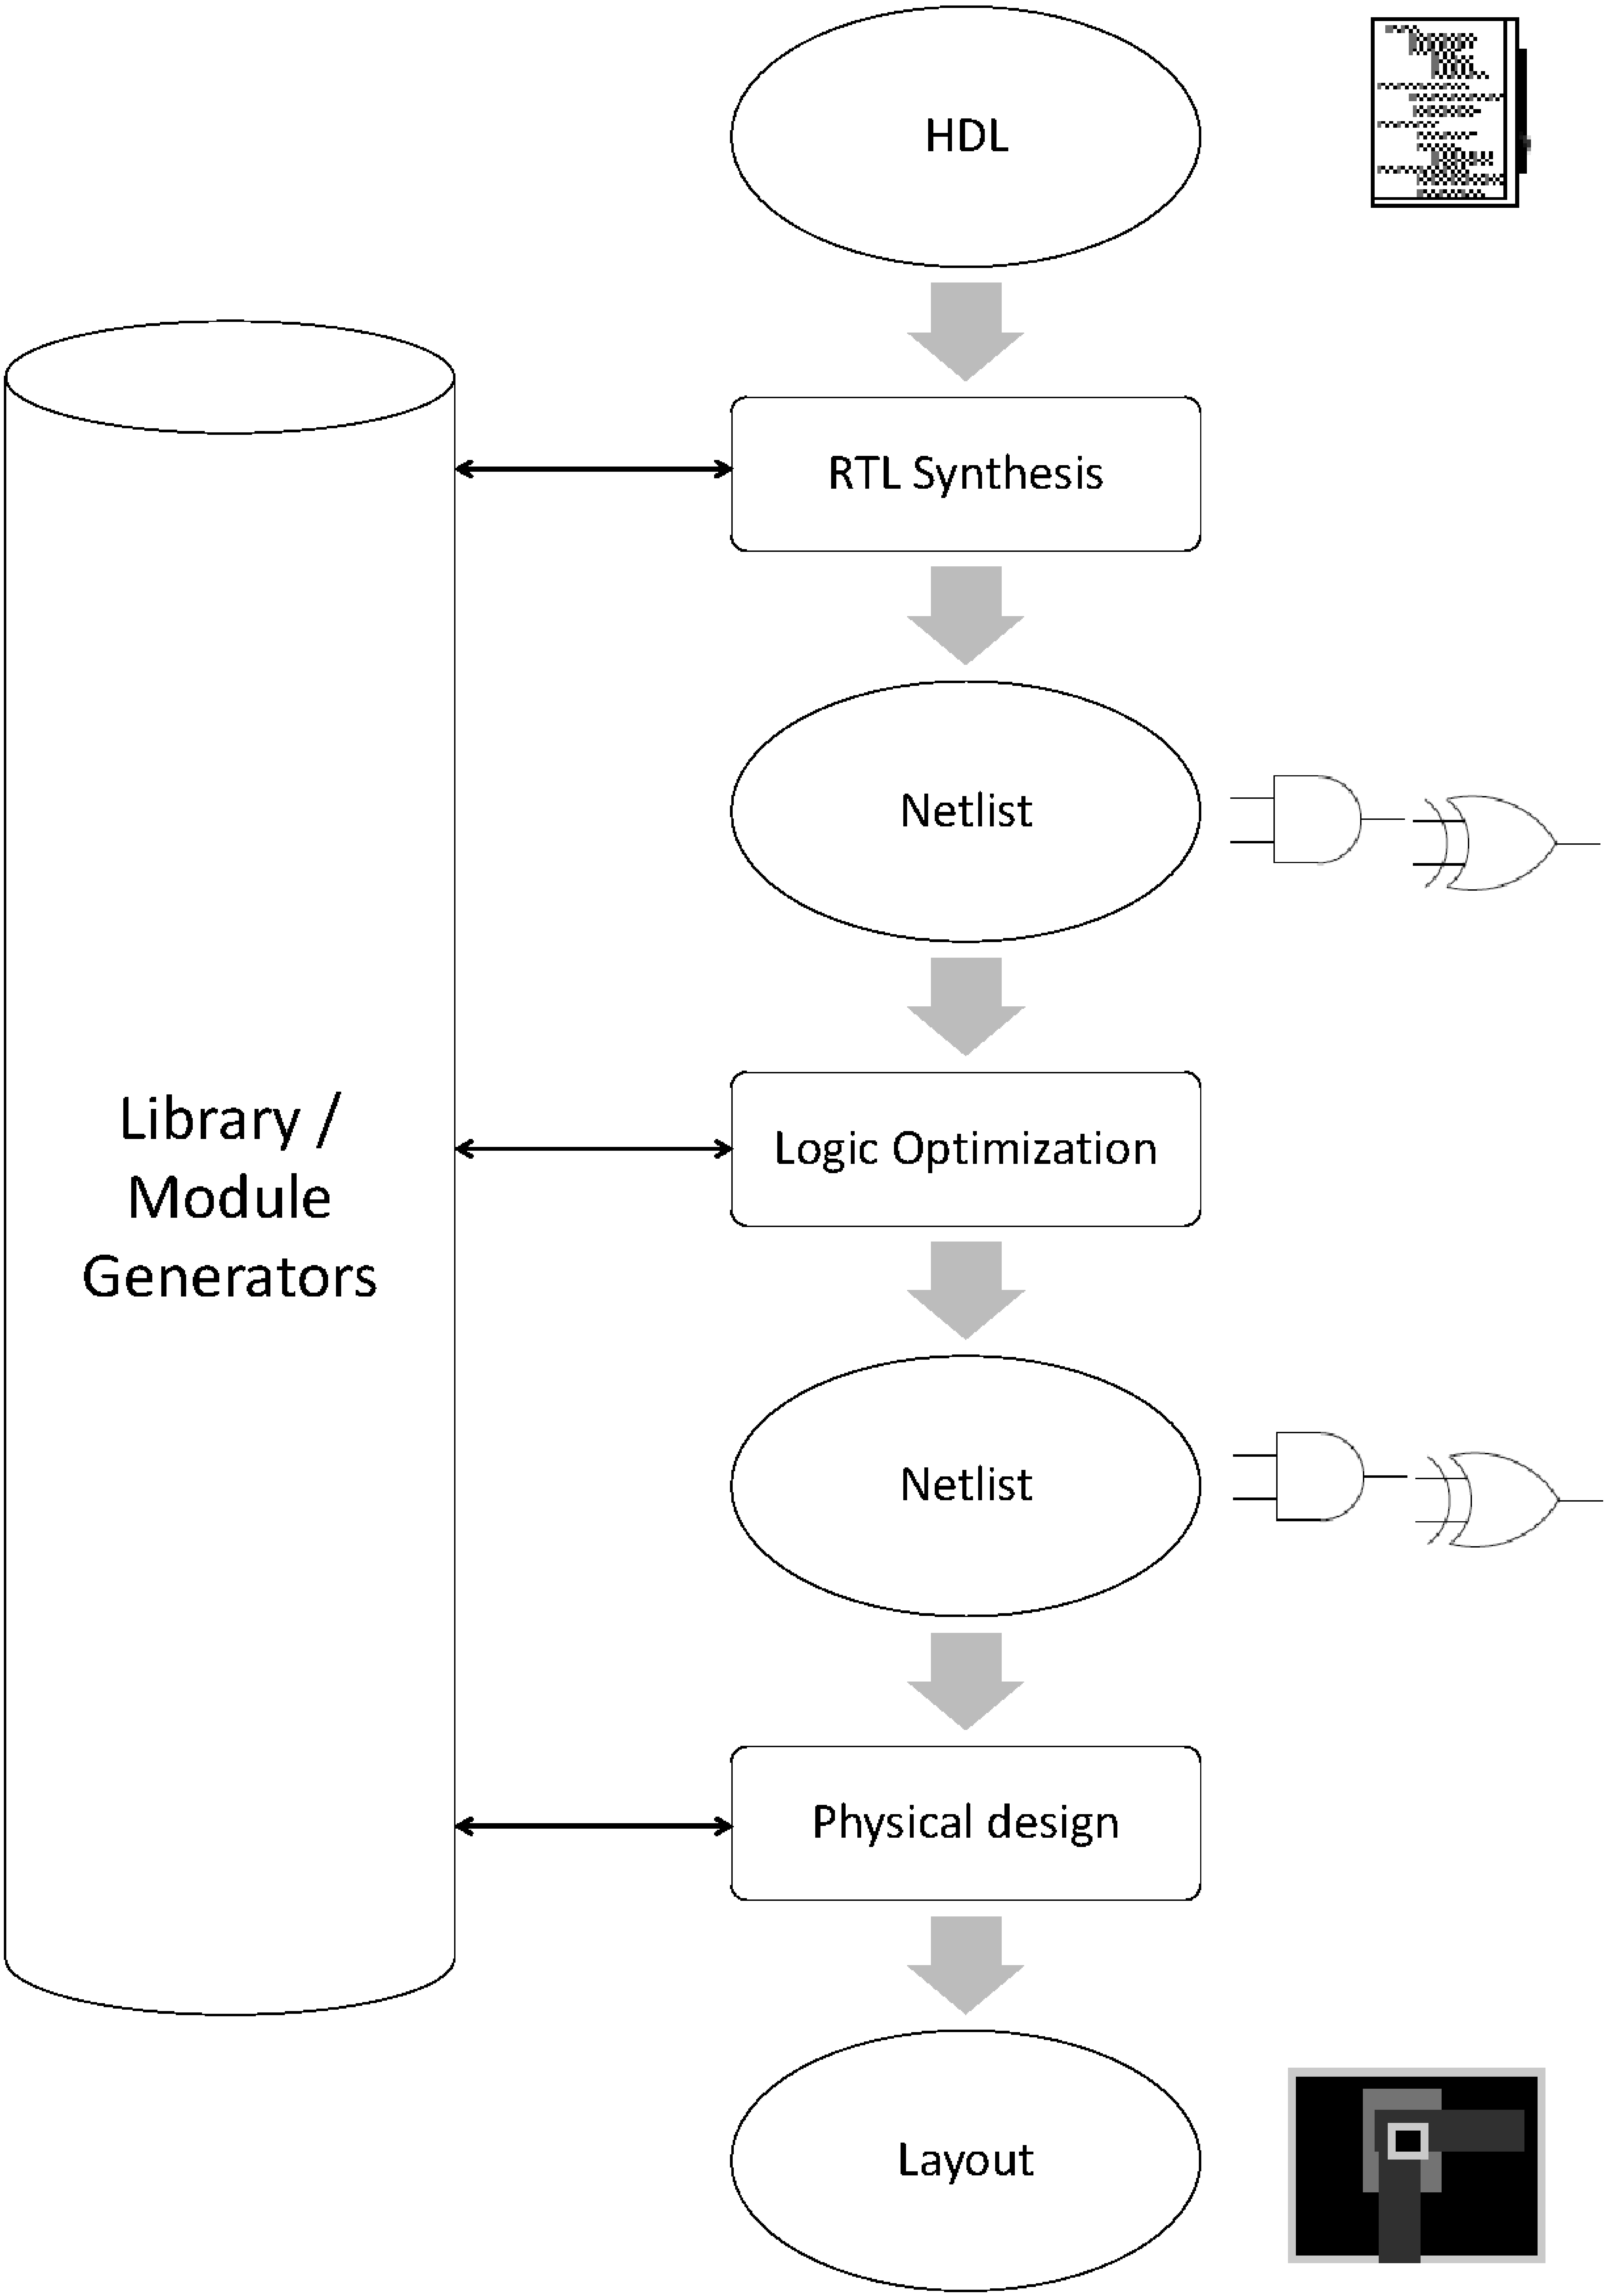
\includegraphics[width=0.7\textwidth]{newfig/designflow.eps}
}
\caption{Typical hardware design flow.}
\label{fig:designflow}
\end{figure}

There are three major
equivalence checking techniques: graph-based,
satisfiability-based (SAT-based) and induction-based.
\begin{enumerate}[{1)}]
\item \emph{Graph-based} techniques compare two circuit implementations 
by representing them using canonical graphs. 
The earliest invented canonical graph is the \emph{Binary Decision Diagram} (BDD) \cite{BRYA86}.
Many variants branch out from BDDs; some widely used variants include 
ZDD \cite{minato1993zero}, BMD \cite{bmd}, FDD \cite{okfdd}, {\it etc.} The comparison algorithms can 
determine whether the two graphs are isomorphic. The canonicity of the graph representation guarantees that
the graphs correspond to the two circuits will be 
equivalent if and only if the circuits implement the same function.
\item \emph{Satisfiability} (SAT) techniques utilize the satisfiability theory.
In circuit equivalence checking, a miter of the two circuits is created.
A \emph{miter} is a combination of the two circuits with one bit-level output, which 
gives output ``1" only when the outputs of the circuits differ with 
the same inputs, {\it e.g. }inputs $a,b,c$ shown in Figure \ref{fig:miter}. 
A SAT solver \cite{csat,mishchenko2006improvements} is then employed to simplify the problem 
and find a satisfying assignment to the inputs for which the 
miter output is ``1". If such an assignment exists, this solution acts as a 
counter-example to equivalence; otherwise the circuits
are functionally equivalent.
\item \emph{Induction-based} techniques are developed and applied to verify the 
equivalence between sequential circuits, which is called the {\it sequential equivalence checking}
(SEC) problem. A miter model can also be built with two sequential circuits. Through the 
miter model, SEC problem is transformed into a sequential backward justification problem.
Equivalence of states and transitions between states can be proved using induction-based 
proof and fix-point calculation \cite{bjesse2000sat,stoffel1997record}.
\end{enumerate}


\begin{figure}[bp]
\centering{
\includegraphics[scale=0.3]{newfig/fig_SAT.eps}
\caption{An example of equivalence checking on miter of circuit $A$ and $B$ using SAT.}
\label{fig:miter}}
\end{figure}

Many formal verification techniques adopt concepts and algorithms from 
\emph{computer-algebra} and \emph{algebraic geometry}.
Algebraic geometry provides a way to reason about the presence or absence of solutions 
without actually solving the system of constraints.
Using methods in \cite{Avrunin:CAV,condrat-tacas07,gbverify:2007,jinpeng,pruss:tcad15}, 
the circuit design can be transformed into a polynomial system. Subsequently, this system
of polynomials is canonicalized by computing a Gr\"obner basis (GB) \cite{gb_book}. 
Computation of GB allows for 
a straightforward proof of important properties of the polynomial system, 
such as the presence or absence of 
solutions. These properties can also be leveraged for 
verification. The disadvantage of the GB computation method is that its complexity can be doubly 
exponential in the worst case \cite{dube1986complexity}. Thus, directly performing GB computation 
over an arbitrary setup is not practical for industry-level applications. However, recent
breakthroughs in computer-algebra hardware verification have shown
that it is possible to overcome the complexity of this computation while
still utilizing the beneficial properties of GB
\cite{lv:phd,tim:phd}.

\section{Importance of Word-level Abstraction}
Most formal verification techniques can benefit from word-level abstractions 
of the circuits they verify.
There are several advantages in exploiting word-level information for
verification. A number of designs have  their
datapaths and/or system-level models described as word-level RTL
models.  Exploiting word-level instead of bit-level information is one
way of abstraction -- a key technique to reduce the state space of a
sequential circuit. It has the effect of combining sets of states with similar 
properties. During reachability analysis, if we use bit-level
variables to  represent the states, the representations may become too
large to handle. However, when a ``bundle" of bit-level variables are
represented as {\it only one word-level variable}, the set of
reachable states can be represented by a  word-level constraint
expression; which may lower verification complexity.

% Abstraction is defined as state-space reduction, i.e{\text . }abstraction
% reduces state-space by mapping the set of states of a system to a smaller 
% set of states. Because the new representation contains fewer states, it
% is easier to comprehend and thus easier to use. 
% Word-level abstraction focuses specifically on abstracting a word-level
% representation of a circuit out of a bit-level representation. For example,
% a bit-level representation of an integer multiplier is represented by a
% collection of Boolean inputs and outputs, whereas a word-level
% abstraction hides the underlying logic and represents the circuit as two 
% integer inputs and one integer output, e.g. $Z=A\cdot B$. As the bit-size of the
% multiplier increases, the logical implementation of the multiplier grows (typically
% exponentially) while the word-level abstraction stays the same.

Word-level abstractions have a wide variety of applications in formal 
verification. For example, it can work as automatic decision and canonical reduction engine in theorem proving;
for RTL composed of macro blocks, abstractions of these blocks also benefit RTL verification.
Concretely, MC and equivalence checking with abstractions can be classified as:
\begin{itemize}  
\item Model checking with abstractions \cite{kroening:model}, 
where an over-approximation of RTL blocks is abstracted and used for property checking on a simplified model.
\item Graph-based equivalence 
checking with abstraction \cite{WLS,arditi:bmd}, where abstraction 
generates a word-level canonical graph representation of the circuit.
\item SAT-based equivalence checking with abstraction \cite{lpsat}, where 
abstractions are used to analyze structural symmetries and similarities such that
the Boolean formulas fed to SAT solver is simplified.
\end{itemize}

Other equivalence checking techniques that employ abstractions 
include {\it satisfiability modulo theory} (SMT) solvers \cite{boolector,bryant:tacas07}.
as well as constraint programming (CP) techniques \cite{ms:research,tew:iccad08}.



Word-level abstractions also find applications in RTL and datapath 
synthesis \cite{demicheli:iccad_98,demicheli:dac_99,demicheli:tcad_03}. 
Since modern datapath design specifications are mostly word-level, synthesis tools with abstractions
can make use of larger macro blocks to generate and optimize the
datapaths. Moreover, 
word-level abstractions facilitates the use of uninterpreted functions (UFs) \cite{UF3}, which 
can be transformed into proposition formulas with word-level information and verified using 
word-level theorem provers and model checkers.

\section{Abstractions in Sequential Design Verification}
With the increasing size of integrated
circuits, sequential circuit designers face complicated problems of
design errors in specification models and implementations. These
errors are usually modeled as ``bad" states, and the
circuits/functional components are modeled as finite state machines
(FSMs). Once state reachability is analyzed, the existence of errors
can be identified by checking whether ``bad" states are {\it
  reachable} from certain initial states. Temporal logic model
  checking formulations and solvers are often used for this
purpose. Once the designs and specification models are validated using
model checking, optimized implementations of sequential circuits are
synthesized. A subsequent problem then needs to be solved to prove
that the sequential circuit implementations are equivalent to the
original specification models, {\it i.e.} {\it Sequential Equivalence
  Checking }(SEC). When the specification is given as an arithmetic function
which canonically represents the circuit, then the problem 
becomes {\it functional verification} of sequential arithmetic circuits.

Reachability analysis forms the backbone of most sequential
verification techniques. As the state-space of FSMs increases,
reachability analysis forms a fundamental bottleneck in sequential
verification. Contemporary approaches employ various techniques to
overcome this state-explosion problem: 

\begin{enumerate}[{1)}]
\item Bounded model checking
\cite{bitlevel1} traverses the FSMs for a fixed number of steps $k$
($k$-BMC) to check whether a property violation can occur in $k$ or
fewer steps.  
\item Analyze over-approximations (or {\it abstractions})
of the state-space. Abstraction proves properties on the system by
first simplifying it, and when the abstraction does not satisfy the
same properties as the original one, a process of refinement is
needed. For example, counterexample guided
abstraction refinement (CEGAR) \cite{cegar-journal} uses proofs of
unsatisfiability (UNSAT cores) to refine the abstractions.
\item The recent breakthrough method of \cite{bradley2011sat} where the set of
over-approximations to forward reachable states are refined with
inductive constraints -- property directed reachability (PDR). 
\end{enumerate}

While the above techniques have made significant strides in sequential
verification, numerous practical instances remain unsolved. One issue
with all of the above techniques is that they mostly use bit-level
constraints to model the transition relations and sets of 
states. Often,
the designs are expressed at the level of bit-vector words
({\it e.g.} Matlab code, Verilog), and these word-level abstractions are
rarely exploited in verification. The problem is further exacerbated
when there are arithmetic operators on word-level operands embedded in
the control logic. While attempts have been made towards word-level
predicate abstraction \cite{jain2005word,mcmillan:cav06,mcmillan2010lazy}, 
{\it using a purely word-level representation
  of the state-space, the properties and their abstractions have not
  been fully explored as another dimension in improving sequential
  verification.}  


   

% Finally, abstractions can also be applied to detect malicious 
% modifications to a circuit, potentially inserted as a hardware trojan horse.
% Hardware trojans, a relatively new security concern in the hardware 
% industry, use certain techniques to add incorrect behavior to a 
% design. 
% This behavior is only activated under certain rare circumstances that only 
% the mal-intent designer has knowledge of.
% The behavior is purposely hidden and is very difficult to encounter during 
% simulation of the design. A manufactured chip with a subsystem 
% that contains a hardware trojan could compromise the entire system in which 
% it is used.
% In some hardware trojan cases, formal verification techniques may be applied 
% to catch a bug in a design and provide a counter-example which exercises it. 
% However, it can be difficult to tell whether the bug in the design was 
% introduced intentionally of not. On the other hand, word-level abstractions 
% of bit-level circuits {\it effectively reverse-engineer the true function 
% implemented by the circuit}, which could be used to determine the designer's 
% true intention.


\section{Objective and Contribution of this Dissertation}
This research proposes a
set of new, promising approaches for {\it word-level representation,
reachability analysis and abstraction} for sequential design verification techniques. 
Our approaches operate at the word-level and are based
largely on the concepts from {\it algebraic geometry}. 

For word-level SEC, we are given two designs, or their corresponding
Mealy/Moore FSMs ${\mathcal{M}}_1,{\mathcal{M}}_2$, along with their
initial starting states $S_0^1,S_0^2$. We wish to prove the absence of
a sequence of inputs (string) that distinguishes the initial
states \cite{coudert:iccad90,coudert1990verification}. Fundamentally, this requires 
the construction of a product machine; and the main research problem
relates to that of performing {\it FSM traversal} \cite{touati1990implicit}
but  at the word-level. Analogously, in the case of MC, the problem
is setup {\it w.r.t.} a FSM $\mathcal{M}$, a set of initial states $S_0$ and
a set of property states $p$. Techniques are to be researched that
verify that there exist no sequence of transitions from an initial
state to a non-property state (``bad'' state). These problems have to
be solved in the context of word-level verification -- {\it i.e.} data
representation, abstraction using UNSAT cores and
algorithm execution has to be carried out at word-level.


\subsection{Word-level Reachability Analysis of FSMs}
In this dissertation, we propose a method to perform reachability analysis at the word-level. 
	The given FSM is modeled as a system of polynomials over a finite field,
	where the state space is mapped to the solutions of the polynomial system.
	Our proposed algorithm utilizes ideal-variety correspondences in algebraic geometry.
	It also forms the foundation for word-level verification by enabling word-level abstraction of the
  state-space.

In this dissertation we represent
the FSMs -- the transition relations -- by means of a set of
multi-variate polynomials with coefficients from the finite (Galois)
field $\Fkk$ of $2^k$ elements, {\it i.e.} polynomials in the ring
$\Fkk[x_1,\dots,x_d]$. Each state of a FSM is identified with a
Boolean assignment to a set of $k$-bit state register variables
$S=\{s_0,\dots,s_{k-1}\}$. Therefore, we can consider each ($k$-bit)
state as a word-level element $S$ of the finite field
$\Fkk$. Algorithms can directly operate on polynomials in word-level
variable $S$. 

Boolean functions with $k$-bit inputs and $k$-bit outputs 
$f: \B^k \rightarrow \B^k,\B = \{0, 1\}$ can be construed as functions
$f: \Fkk \rightarrow \Fkk$. It is well-known that over the finite
field ($\Fq$) of  $q$ elements, every function $f: \Fq
\rightarrow \Fq$ is a polynomial function \cite{ff:1997}. Moreover,
there exists a unique canonical polynomial $\Func$ that describes $f$.
This implies that one can derive a canonical, polynomial
  abstraction of the function as $Z = \Func(A)$ where $Z, A$ are
word-level symbols representing $k$-bit operands. The concept also
generalizes to functions with different input/output bit-vector sizes,
{\it i.e.} functions of the type $f: \B^n \rightarrow \B^m$, modeled as
polynomials over $f:{\mathbb{F}}_{2^k} \rightarrow
{\mathbb{F}}_{2^k}$, where $k=LCM(n,m)$ \cite{ff:1997}.  
{\it This implies that the FSM's transition relations can be
represented as polynomial functions (ideals) in $\Fkk$, and values of
state variables can be represented as solutions to these polynomials}
(variety of the ideal). Subsequently, the ideal-variety correspondences
in algebraic geometry can be applied to implement symbolic reasoning
about state reachability. 
% Moreover, as ${\mathbb{F}}_2 \subset \Fkk$,
% our model provides a single, unified and bit-precise representation
% for both bit-level (${\mathbb{F}}_2$) and word-level ($\Fkk$)
% constraints.  

The decision and abstraction procedures in our setting will rely on
the theory and technology of {\it \Grobner bases}. GB-based
algebraic reasoning is very powerful; in fact it is known to be
strictly stronger than resolution \cite{CEI:stoc-96}. Therefore, in
light of the above discussion, using concepts from algebraic geometry
and \Grobner bases over $\Fkk$, we can introduce another dimension of
word-level abstraction to the techniques in sequential verification. 
This work was published at \cite{myHLDVT}.

\subsection{Application to Sequential Galois Field Arithmetic Circuit Verification}
Sequential Galois field (GF) arithmetic circuits can be modeled as a special type of 
FSM, where the pre-loaded operands are mapped to initial states, and pseudo outputs
after $k$ clock-cycles are recognized as the final reached state after $k$ transitions.
Therefore, the word-level FSM traversal algorithm can be applied to 
verify the correctness of final reached state, {\it i.e.} the functional correctness of
a sequential arithmetic circuit.

In our proposed approach, word-level abstraction is employed to generate, in every time-frame, the 
word-level signature of the combinational logic component of the sequential 
arithmetic circuit. This abstraction requires a GB computation, which usually has high time/space 
complexity. We propose several improvements to simplify the GB computation procedure
and make the entire algorithm execution practical. As a result, we successfully verify sequential 
multipliers with 162-bit datapaths. This work was published at \cite{myDATE} and a journal paper
is under preparation.

\subsection{UNSAT Cores in Algebraic Geometry}
Abstraction is an effective method to lower the cost to traverse the state space.
In modern model checkers, abstraction is used to simplify and refine the model 
during the iterative execution of the tool. An UNSAT core is widely used 
as an important component of abstraction refinement. The reason is that UNSAT cores can provide 
information about the state variables that truly affect the property, 
and that information is necessary for the refinement process. 

In this dissertation, we explore the concept, and the computation, of unsatisfiable (UNSAT)
  cores of  a set of polynomials using the Gr\"obner bases algorithm. We also propose
a number of heuristics that extend the Buchberger's algorithm to reduce the size of UNSAT core. 
  We demonstrate the use of UNSAT core extraction 
  to a bounded model checking instance with abstraction refinement.
 This work was published at \cite{myCP}.

% \subsection{Dissertation Contributions}
% In this dissertation, we focus on sequential circuit verification problems and 
% propose solutions consisting of three main contributions: 
% \begin{enumerate}[{1)}]
% \item A method to perform reachability analysis at the word-level. 
% 	The given FSM is modeled as a system of polynomials over finite field,
% 	where the state space is mapped to its solution space.
% 	Our proposed algorithm utilize concepts in algebraic geometry including ideals and varieties.
% 	It also forms the foundation for word-level SEC and MC by enabling word-level abstraction of the
%   state-space.
% \item Using the theory of FSM traversal, we apply the algorithm to verify the 
% function of sequential GF arithmetic circuits. Our proposed approach uses GB-engines efficiently 
% and can verify sequential multipliers with 162-bit datapaths.
% \item We explore the concept, and the computation, of unsatisfiable (UNSAT)
%   cores of  a set of polynomials using Gr\"obner bases calculation. We apply the UNSAT core extraction 
%   to abstraction-refinement
%   techniques such as bounded model checking (BMC). 
% \end{enumerate}

\section{Dissertation Organization}
The rest of the dissertation is organized as
follows: Chapter \ref{ch:prev} reviews previous work, and analyzes their drawbacks with respect to 
the word-level sequential verification problem.
Chapter \ref{ch:prelim_GF} covers preliminary
concepts and notation on finite fields, and the methodology about design of arithmetic circuits in finite fields.
Chapter \ref{ch:ideals} provides a theoretical background on algebraic geometry and Gr\"obner bases.
Chapter \ref{ch:reacha} describes the basic
concept of word-level FSM traversal and introduces our proposed word-level FSM traversal algorithm. 
Chapter \ref{ch:normal} explores the application of FSM traversal algorithm on 
functional verification of sequential GF arithmetic circuits. Chapter \ref{ch:UNSAT} describes
algorithmic techniques to derive UNSAT cores of polynomial
ideals. It also demonstrates with the help of an example how abstraction via
UNSAT cores in algebraic geometry can simplify BMC. 
Chapter \ref{ch:conclude} outlines potential future research for
continuation of this work and concludes the dissertation. 
An appendix provides theory and methodology on the characterization of finite field normal basis,
as well as the construction of optimal normal basis and application to normal basis multiplier design.
\chapter{Previous Work}
\label{ch:prev}
\section{SAT,DD,AIG-based Sequential Circuit Verification}

\section{Bounded Model Checking}

\section{Model Checking with Abstraction Refinement}

\section{Word-level Techniques in Sequential Circuit Verification}
Term rewriting?

\section{Verification of Galois Field Circuits}

\section{Conventional UNSAT Core Extraction}

\section{Conclusion Remarks}
\chapter{Finite Fields and Sequential Arithmetic Circuits}
\label{ch:prelim_GF}
This chapter provides a mathematical background for understanding 
finite fields (Galois fields) and explains how to design Galois field (GF) arithmetic circuits.
We first introduce the mathematical concepts of groups, rings, fields, and 
polynomials. 
We then apply these concepts to create Galois field arithmetic functions and 
explain how to map them to a Boolean circuit implementation.
Additionally, we introduce a special type of sequential arithmetic hardware based on normal basis, as well
as the normal basis theory behind the designing such hardware.

The material is referred from \cite{galois_field:mceliece, ftheory:2006, ff:1997} for Galois field concepts, 
\cite{mastro:1989, PT:1985, acar:1998, wu:2002, Knezevic:2008} for hardware design over Galois fields 
and previous work by Lv \cite{lv:phd}.
Normal basis theory in this section is referred from \cite{normal_book, gao:phd_normal_basis} and sequential
normal basis arithmetic hardware designs come from \cite{mullinONB,MasseyOmura,agnew1991implementation, RHmulti}.

\section{Commutative Algebra}
\label{sec:algebra}
\subsection{Group, Ring and Field}
\begin{Definition}
An {\bf Abelian group} is a set $\mathbb{S}$ with a binary operation $'+'$
which satisfies the following properties: 
\begin{itemize}
\item {\it Closure Law:} For every $a, b \in \mathbb{S}, a + b \in \mathbb{S}$  
\item {\it Associative Law:} For every $a, b, c \in \mathbb{S}, (a + b) + c = a + (b + c)$
\item {\it Commutativity:} For every $a, b \in \mathbb{S}, a + b = b + a$. 
\item {\it Additive Identity:} There is an identity element $0 \in \mathbb{S}$
such that for all $a \in \mathbb{S};$ $a + 0 = a$.
\item {\it Additive Inverse:} If $a \in \mathbb{S}$, then there is an
element $a^{-1} \in \mathbb{S}$ such that $ a + a^{-1} = 0$.
\end{itemize}
\end{Definition}

The set of integers $\mathbb{Z}$ forms an Abelian group under the addition operation. 

\begin{Definition}
Given a set $\mathbb{R}$ with two binary operations, $'+'$ and $'\cdot'$, 
and element $0 \in \mathbb{R}$, the system $\mathbb{R}$ is called a {\bf commutative ring with unity} if the following properties hold:
\begin{itemize}
\item $\mathbb{R}$ forms an Abelian group under the '+' operation with additive identity element $0$.
\item {\it Multiplicative Distributive Law}: For all $a, b, c \in$ $\mathbb{R}$, $a\cdot (b + c) = a\cdot b + a\cdot c$.
\item {\it Multiplicative Associative Law}: For every $a, b, c\in \mathbb{R}$, $a\cdot (b\cdot c) = (a\cdot b)\cdot c$. 
\item {\it Multiplicative Commutative Law}: For every $a,b \in \mathbb{R}$, $a\cdot b = b\cdot a$
\item {\it Identity Element}: There exists an element $1 \in$ $\mathbb{R}$ 
such that for all $a \in \mathbb{R}$, $a\cdot 1 = a =1\cdot a$
\end{itemize}
\end{Definition}

{\bf Ring} is a broad algebraic concept. In this dissertation, this word is used to refer a special 
sort of ring -- {\bf commutative ring with unity}. Two common 
examples of such rings are the set of integers, $\mathbb{Z}$, and the set of 
rational numbers, $\mathbb{Q}$. While both of these examples are
rings with an infinite number of elements, the number of elements in a ring 
can also be finite, such as the ring of integers modulo $n$ ($\Z_n$).

\begin{Definition}
A {\bf field} $\mathbb{F}$ is a commutative ring with unity, where every
non-zero element in $\mathbb{F}$ has a multiplicative inverse; {\it i.e.} $\forall
a \in \mathbb{F} - \{0\}$, $\exists \hat{a} \in \mathbb{F}$ such that $ a \cdot
\hat{a} = 1$.
\end{Definition}

A field is defined as a ring with one extra condition: the presence of a 
multiplicative inverse for all non-zero elements.
Therefore, a field must be a ring while a ring is not necessarily a field.
For example, the set $\mathbb{Z}_{2^k} = \{0,1,\cdots, 2^k-1\}$ forms a finite ring.
However, $\mathbb{Z}_{2^k}$ is not a field because not every element in
$\mathbb{Z}_{2^k}$ has a multiplicative inverse. 
In the ring $\mathbb{Z}_{2^3}$, for 
instance, the element $5$ has an inverse ($5\cdot5\pmod{8}=1$) but the element $4$
does not.

An important concept in field theory is {\bf field extension}. The idea behind a
field extension is to take a base field and construct a larger field which 
contains the base field as well as satisfies additional properties. For example,
the set of real numbers $\mathbb{R}$ forms a field; one extension of 
$\mathbb{R}$ is the set of complex numbers $\mathbb{C}=\mathbb{R}(i)$. Every
element of $\mathbb{C}$ can be represented as $a+b\cdot i$ where $a,b \in \mathbb{R}$,
hence $\mathbb{C}$ is a two-dimensional extension of $\mathbb{R}$.

Like rings, fields can also contain either an infinite or a finite number of 
elements. 
In this dissertation we focus on finite fields -- also known as Galois fields, 
the construction of their field extensions, and their applications on circuit verification and abstraction techniques.

\subsection{Finite Field}
Finite fields find widespread applications in 
many areas of electrical engineering and computer science such as error-
correcting codes, elliptic curve cryptography, digital signal processing, 
testing of VLSI circuits, among others.
In this dissertation, we specifically focus on their application to 
the FSM traversal of sequential Galois field circuits as well as abstraction refinement based on UNSAT core extraction.
This section describes the relevant Galois field concepts
\cite{galois_field:mceliece} \cite{ftheory:2006} \cite{ff:1997}
and hardware arithmetic designs over such fields \cite{mastro:1989} \cite{PT:1985} 
\cite{acar:1998} \cite{wu:2002} \cite{Knezevic:2008}. 

%%%%%%%%%%%%%%%%%%%%%%%%%%%%%%%%%%%%%%%%%%%%%%%%%%%%%%%%%%%%%%%%%%%%%%%%%%%%

\begin{Definition} 
A {\bf Galois field}, denote $\Fq$, is a field with a finite
number of elements, $q$. The number of elements $q$ of the field is
a power of a prime integer, {\it i.e.} $q = p^k$, where $p$ is a prime
integer, and $k \geq 1$. Thus a Galois field can also be denoted as 
$\F_{p^{k}}$.
\end{Definition}

Fields of the form $\F_{p^{k}}$ are called Galois extension fields.
We are specifically interested in extension fields of type 
$\Fkk$, where $k > 1$, because they are extensions of the binary
field $\F_2$. Elements and operators in $\F_2$ can be mapped to 
Boolean values and Boolean operators, as Table \ref{tab:1stTab} shows.
Notice that addition over $\F_2$ is a Boolean {\sc XOR} operation, 
because it is performed modulo $2$.
Similarly, multiplication over $\F_2$ performs a Boolean {\sc AND} operation.

\begin{table}[bp]
% \vspace{-0.3cm}
\caption{Addition and multiplication operations over $\F_2$.\vspace{0.5cm}}
	\centering
	\label{tab:1stTab}
	\begin{tabular}{m{1cm}|l|ll|m{1cm}}
% 	\indent\\
	\hhline{~---~}
	\multirow{3}{*}{} & $+$ & $0$ & $1$ & \multirow{3}{*}{} \\
	\hhline{~---~}
	& $0$ & $0$ & $1$ & \\
	& $1$ & $1$ & $0$ & \\
	\hhline{~---~}
	\multicolumn{5}{c}{}\\
	\multicolumn{5}{c}{Addition over $\F_2$}\\
	\end{tabular}
	\quad
	\begin{tabular}{m{1cm}|l|ll|m{1cm}}
% 	\indent\\
	\hhline{~---~}
	\multirow{3}{*}{} & $\cdot$ & $0$ & $1$ & \multirow{3}{*}{} \\
	\hhline{~---~}
	& $0$ & $0$ & $0$ & \\
	& $1$ & $0$ & $1$ & \\
	\hhline{~---~}
	\multicolumn{5}{c}{}\\
	\multicolumn{5}{c}{Multiplication over $\F_2$}\\
	\end{tabular}
	
	
\end{table}

Algebraic extensions of the binary field $\F_{2}$  
are generally termed as {\it binary extension fields} $\Fkk$.
Where elements in $\F_2$ can only represent $1$ bit, elements in $\Fkk$ 
represent a $k$-bit vector.
This allows them to be widely used in digital hardware applications.
In order to construct a Galois field of the form $\Fkk$, 
an {\bf irreducible polynomial} is required:
\begin{Definition}
A polynomial $P(x) \in \mathbb{F}_{2}\left[x\right]$, {\it i.e.} the set of all 
polynomials in $x$ with coefficients in $\F_2$, is {\bf irreducible} 
if $P(x)$ is non-constant with degree $k$ and cannot be 
factored into a product of polynomials of lower degree in $\mathbb{F}_2[x]$.
\end{Definition}

Therefore, the polynomial $P(x)$ with degree $k$ is irreducible over 
$\mathbb{F}_{2}$ if and only if it has no roots in $\mathbb{F}_{2}$,
i.e if $\forall a \in \mathbb{F}_{2}$, $P(a)\neq 0$.
For example, $x^2+x+1$ is an irreducible polynomial over $\mathbb{F}_{2}$
because it has no solutions in $\mathbb{F}_{2}$, {\it i.e.} $(0)^2+(0)+1=1\neq0$ 
and $(1)^2+(1)+1=1\neq0$ over $\F_2$.
Irreducible polynomials exist for any degree $\geq 2$ in $\mathbb{F}_2[x]$.

Given an irreducible polynomial $P(x)$ of degree $k$ in the polynomial ring 
$\mathbb{F}_2[x]$, we can construct a binary extension field 
$\mathbb{F}_{2^k} \equiv \mathbb{F}_2[x] \pmod{P(x)}$.
Let $\alpha$ be a root of $P(x)$, {\it i.e.} $P(\alpha)=0$.
Since $P(x)$ is irreducible over
$\mathbb{F}_2[x]$, $\alpha \notin \mathbb{F}_2$. 
Instead, $\alpha$ is an element in $\mathbb{F}_{2^k}$. 
Any element $A \in \mathbb{F}_{2^k}$ is then represented as: 
\begin{equation}\label{rep:poly}
A= \sum_{i=0}^{k-1} (a_i \cdot \alpha^i) = a_0 + a_1\cdot\alpha + \cdots + a_{k-1}\cdot \alpha^{k-1}\nonumber
\end{equation}
where $a_i \in \mathbb{F}_2$ are the coefficients and $P(\alpha)=0$.

To better understand this field extension, compare its similarities to another
common-place
field extension $\C$, the set of complex numbers. $\C$ is an extension of the field 
of real numbers $\R$ with an additional element $i=\sqrt{-1}$, which is an imaginary
root in the algebraic closure of $\R$ -- the closure is known as the field of complex numbers $\C$.
Thus $i \notin \R$, rather $i \in \C$.
Every element $A \in \mathbb{C}$ can be represented as:
\begin{equation}\label{rep:polyC}
A=\sum_{j=0}^{1} (a_j \cdot i^j)=a_0+a_1\cdot i
\end{equation}
where $a_j \in \R$ are coefficients. Similarly, $\Fkk$ is an extension of $\F_2$ with 
an additional element $\alpha$, which is the ``imaginary root'' of an irreducible 
polynomial $P$ in $\F_2[x]$.

Every element $A \in \Fkk$ has a degree less than $k$ because 
$A$ is always computed modulo $P(x)$, which has degree $k$. 
Thus, $A\pmod {P(x)}$ can be of degree at most $k-1$ and at least $0$.
For this reason, the field $\mathbb{F}_{2^k}$ can be viewed as a $k$
dimensional vector space over $\mathbb{F}_{2}$. 
The equivalent bit vector representation for element $A$ is:
\begin{equation}
A=(a_{k-1} a_{k-2} \cdots a_{0})
\end{equation}

\begin{Example}
A 4-bit Boolean vector, $(a_{3} a_{2} a_{1} a_{0})$
can be presented over $\F_{2^4}$ as: 
\begin{equation}
a_3 \cdot \alpha^3+a_2 \cdot \alpha^2+a_1 \cdot \alpha+a_0
\end{equation}
For instance, the Boolean vector $1011$ is represented as the element 
$\alpha^3+\alpha+1$.
\end{Example}

\begin{Example}\label{exp:1}
Let us construct $\mathbb{F}_{2^4}$ as $\mathbb{F}_2[x] \pmod{ P(x)}$, where
$P(x)=x^4+x^3+1 \in \mathbb{F}_2[x]$ is an irreducible polynomial of degree $k=4$. 
Let $\alpha$ be the root of $P(x)$, {\it i.e.} $P(\alpha)=0$. 

Any element $A \in \mathbb{F}_2[x] \pmod{ x^4 + x^3 + 1}$
has a representation of the type: $A = a_3 x^3 + a_2 x^2 +
a_1 x + a_0$ (degree $< 4$) where the coefficients $a_3, \dots, a_0$ are in $\F_2 =
\{0, 1\}$. Since there are only $16$ such polynomials, we obtain
$16$ elements in the field $\mathbb{F}_{2^4}$. Each element in
$\mathbb{F}_{2^4}$ can then be viewed as a $4$-bit vector over $\mathbb{F}_{2}$. 
Each element also has an exponential $\alpha$
representation. All three representations are shown in Table
\ref{tab:gfelement}.

\begin{table}[bp]
\begin{center}
\caption{Bit-vector, Exponential and Polynomial representation of
elements in  $\mathbb{F}_{2^4} = \mathbb{F}_2[x] \pmod{x^4+x^3+1}$.}\label{tab:gfelement} 
\begin{tabular}{|c|c|c||c|c|c|} 
\hline
$a_3a_2a_1a_0$ & Exponential & Polynomial     &$a_3a_2a_1a_0$ & Exponential & Polynomial  \\
\hline
$0000$        & $0$         & $0$            & $1000$ & $\alpha^3$ &  $\alpha^3$\\
\hline
$0001$        & $1$         & $1$            & $1001$ & $\alpha^4$ & $\alpha^3 + 1$\\
\hline
$0010$        & $\alpha$    & $\alpha$       & $1010$ & $\alpha^{10}$&$\alpha^3 + \alpha$  \\
\hline
$0011$        & $\alpha^{12}$& $\alpha + 1$   & $1011$ & $\alpha^5$ & $\alpha^3+\alpha+1$\\
\hline
$0100$        & $\alpha^2$  & $\alpha^2$     &  $1100$ & $\alpha^{14}$ & $\alpha^3 + \alpha^2$\\
\hline
$0101$        & $\alpha^9$   &$\alpha^2 + 1$ & $1101$  &$\alpha^{11}$  & $\alpha^3+\alpha^2+1$\\
\hline
$0110$        & $\alpha^{13}$& $\alpha^2 + \alpha$ & $1110$ & $\alpha^8$& $\alpha^3+\alpha^2+\alpha$\\
\hline
$0111$        &$\alpha^7 $ & $\alpha^2+\alpha+1$ & $1111$ &$\alpha^6$ & $\alpha^3+\alpha^2+\alpha+1$\\
\hline
\end{tabular}
\end{center}
\end{table}

We can compute the polynomial representation from the exponential representation.
Since every element is computed $\pmod{P(\alpha)} = \pmod{\alpha^4+\alpha^3+1}$, 
we compute the element $\alpha^{4}$ as 
\begin{equation}
\alpha^{4} \pmod{ \alpha^4+\alpha^3+1} = -\alpha^3 - 1 = \alpha^3+1
\end{equation}
Recall that all coefficients of $\F_{2^4}$ 
are in $\F_{2}$ where $-1 = +1$ modulo 2.
The next element $\alpha^{5}$ can be computed as 
\begin{equation}
\alpha^{5} = \alpha^{4}\cdot \alpha = (\alpha^3+1)\cdot \alpha = \alpha^4+\alpha = \alpha^3+\alpha+1 
\end{equation}
Then $\alpha^6$ can be computed as $\alpha^{5}*\alpha$ and so on.
\end{Example}

An irreducible polynomial can also be a primitive polynomial.

\begin{Definition}
A {\bf primitive polynomial} $P(x)$ is a polynomial with coefficients in $\mathbb{F}_2$ 
which has a root $\alpha$ $\in$ $\mathbb{F}_{2^k}$
such that \{$0$, $1(=\alpha^{{2^k}-1})$, $\alpha$, $\alpha^2$, $\cdots$, $\alpha^{2^k-2}$\} is the set of 
all elements in $\mathbb{F}_{2^k}$.
Here $\alpha$ is called a {\bf primitive element} of $\mathbb{F}_{2^k}$. 
\end{Definition}

A primitive polynomial is guaranteed to generate all distinct elements 
of a finite field $\mathbb{F}_{2^k}$ while an arbitrary irreducible polynomial
has no such guarantee.
Often, there exists more than one irreducible polynomial of degree $k$.
In such cases, any degree $k$ irreducible polynomial can be 
used for field construction. For example, both $x^3+x+1$ and $x^3+x^2+1$ 
are irreducible in $\mathbb{F}_2$ and either one can be used
to construct $\mathbb{F}_{2^3}$. This is due to the following:

\begin{Theorem}\label{the:unique}
There exist a {\bf unique} field $\mathbb{F}_{p^k}$, for any prime $p$ and any positive integer $k$.
\end{Theorem}

Theorem \ref{the:unique} implies that Galois fields with the same number of elements are 
{\bf isomorphic} to each other up to the labeling of the elements. 

Theorem \ref{the:fer} provides an important property for investigating solutions to
polynomial equations in $\Fq$.

\begin{Theorem}\label{the:fer}
 $\left[Generalized\  Fermat's\  Little\  Theorem \right]$ Given a
 Galois field $\mathbb{F}_{q}$, each element $A \in \mathbb{F}_{q}$ satisfies: 
\begin{eqnarray}\label{fe}
 A^{q} & \equiv & A  \nonumber \\
 A^{q} - A & \equiv& 0  
\end{eqnarray}
\end{Theorem} 

We can extend Theorem \ref{the:fer} to polynomials in $\mathbb{F}_{q}[x]$ as 
follows: 
\begin{Definition}
Let $x^q-x$ be a polynomial in $\mathbb{F}_{q}[x]$.
Every element $A \in \mathbb{F}_{q}$ is a solution to  $x^q-x=0$. 
Therefore, $x^{q} - x$ always {\it vanishes} in $\mathbb{F}_{q}$. Such 
polynomials are called {\bf vanishing polynomials} of the field $\mathbb{F}_{q}$.
\end{Definition}

\begin{Example}
Given $\mathbb{F}_{2^2} =\{0,1,\alpha,\alpha+1\}$ with $P(x)=x^2+x+1$, where $P(\alpha)=0$. 
 \begin{eqnarray}
 0^{2^2}&=&0 \nonumber \\
 1^{2^2}&=&1 \nonumber \\
 \alpha^{2^2}&=&\alpha \pmod {\alpha^2+\alpha+1}\nonumber \\
 (\alpha+1)^{2^2}&=&\alpha+1 \pmod {\alpha^2+\alpha+1} \nonumber 
 \end{eqnarray}
\end{Example}

A Galois field $\F_q$ can be fully contained within a larger field $\F_{q^k}$.
That is, $\F_q \subset \F_{q^k}$.
For example, the containment relation of the fields 
$\F_2 \subset \Fkk$ is usually used to represent bit-level Boolean variables as field elements
in larger finite field which allows projection of $k$-bit word-level variables. 
Concretely, $\F_{16}=\F_{4^2}=\F_{2^4}$ contains $\F_4$ and $\F_2$.
The elements $\{0,1,\alpha,\dots,\alpha^{14}\}$
designate $\F_{16}$. Of these, $\{0,1,\alpha^5,\alpha^{10}\}$ create $\F_4$.
From these, only $\{0,1\}$ exist in $\F_2$.

\begin{Theorem}
$\F_{2^n}\subset\F_{2^m}$ iff $n \mid m$, {\it i.e.} if $n$ divides $m$.
\end{Theorem}

Therefore:
\begin{itemize}
\item $\F_2 \subset \F_{2^2} \subset \F_{2^4} \subset \F_{2^8} \subset \dots$
\item $\F_2 \subset \F_{2^3} \subset \F_{2^9} \subset \F_{2^{27}} \subset \dots$
\item $\F_2 \subset \F_{2^5} \subset \F_{2^{25}} \subset \F_{2^{125}} \subset \dots,$ and so on
\end{itemize}

\begin{Definition}
The {\bf algebraic closure} of the Galois field $\F_{2^k}$, denoted $\overline{\Fkk}$, is the 
union of all fields $\F_{2^n}$ such that $k \mid n$.
\end{Definition}

\section{Normal Basis Multiplier over Galois Field}
From an algebraic perspective, a field is a space, and field elements are points in the space. Those elements can be 
represented with unique coordinates, which requires the pre-definition of a basis vector. In this
section, we discuss a special basis called normal basis, as well as the advantages adopting it in 
GF operations, especially multiplication.
\subsection{Normal Basis}
Given a Galois field $\Fkk$ is a finite field with  $2^k$ elements and characteristic equals to 2.
Its elements can be written in polynomials of $\alpha$, when there is an irreducible polynomial $p(\alpha)$
defined.

If we use a basis $\{1,\alpha,\alpha^2,\alpha^3,\dots,\alpha^{k-1}\}$, we can easily transform polynomial representations
to binary bit-vector representations by recording the coefficients. For example, for elements in
$\F_{2^4}$, the results are shown in Table \ref{tab:gfelement}, column ``Polynomial".

% \begin{table}[H]
% \centering
% \caption{Bit-vector, Exponential and Polynomial representation of
% elements in  ${\mathbb{F}}_{2^4} = {\mathbb{F}}_2[x]
% \pmod{x^4+x^3+1}$}
% \begin{tabular}{|c|c||c|c|} 
% \hline
% $a_3a_2a_1a_0$ & Polynomial     &$a_3a_2a_1a_0$ & Polynomial  \\
% \hline
% $0000$        & $0$           & $1000$  &$\alpha^3$\\
% \hline
% $0001$        & $1$           & $1001$  & $\alpha^3 + 1$\\
% \hline
% $0010$        &  $\alpha$       & $1010$ & $\alpha^3 + \alpha$  \\
% \hline
% $0011$        &  $\alpha + 1$   & $1011$ &  $\alpha^3+\alpha+1$\\
% \hline
% $0100$        &  $\alpha^2$     &  $1100$ &  $\alpha^3 + \alpha^2$\\
% \hline
% $0101$        & $\alpha^2 + 1$ & $1101$  & $\alpha^3+\alpha^2+1$\\
% \hline
% $0110$        &  $\alpha^2 + \alpha$ & $1110$ &  $\alpha^3+\alpha^2+\alpha$\\
% \hline
% $0111$        & $\alpha^2+\alpha+1$ & $1111$ & $\alpha^3+\alpha^2+\alpha+1$\\
% \hline
% \end{tabular}
% \label{table:booltogalois}  
% \end{table}

The basis $\{1,\alpha,\alpha^2,\alpha^3,\dots,\alpha^{k-1}\}$ is called a {\bf standard basis} (StdB), which results in
a straightforward representation for elements, and operations of elements such as addition and subtraction.
The addition/subtraction of GF elements in StdB follows the rules of polynomial addition/subtraction
where coefficients belong to $\mathbb F_2$. In other words, using the definition of {\it exclusive or} (XOR) in
Boolean algebra, element $A$ add/subtract by element $B$ in StdB is defined as
\begin{align}\label{eqn:StdB}
A+B = A-B &= (a_0,a_1,\dots,a_{k-1})_{StdB} \xor (b_0,b_1,\dots,b_{k-1})_{StdB} \nonumber\\
&=(a_0\oplus b_0, a_1\oplus b_1,\dots,a_{k-1}\oplus b_{k-1})_{StdB} 
\end{align}

\subsection{Multiplication using Normal Basis}
Besides addition/subtraction, multiplication is also very common in arithmetic circuit design.
The multiplication of GF elements in $\Fkk$ in StdB follows the rule of polynomial multiplication.
However, it will result in $O(k^2)$ bitwise operations. In other words, if we implement GF multiplication
in a bit-level logic circuit, it will contain $O(k^2)$ gates. When the datapath size $k$ is large,
the area and delay of circuit will be costly.

In order to lower the complexity of arithmetic circuit design, Massey and Omura \cite{MasseyOmura} % ref 7 in RH paper
use a new basis to represent GF elements, which is called a {\bf normal basis} (NB).
A normal basis over $\Fkk$ is written in the form of
\begin{equation*}
N.B. ~~~ \N = \{\beta,\beta^2,\beta^4,\beta^8,\dots,\beta^{2^{k-1}}\}
\end{equation*}

{\bf Normal element} $\beta$ is an element from the field which is used to construct the normal basis,
and can be represented as a power of the primitive element $\alpha$: 
\begin{equation*}
\beta = \alpha^t, ~~~ 1\leq t<2^k
\end{equation*}
Exponent $t$ takes values in the given range when $\N$ fulfills the definition of a basis.

Correspondingly, a field element in NB representation is actually
\begin{align*}
A &= (a_0,a_1,\dots,a_{k-1})_{NB} \\
  &= a_0\beta+a_1\beta^2+\cdots+a_{k-1}\beta^{2^{k-1}} \\
  &= \sum_{i=0}^{k-1} a_i\beta^{2^i}
\end{align*}

According to the definition, a normal basis is a vector where the next entry is the square of the former one.
We note that the vector is cyclic, {\it i.e.} $\beta^{2^k} = \beta$ due to {\it Fermat's little theorem}.

The addition and subtraction of elements in NB representation are similar to Equation \ref{eqn:StdB}.
However, what makes NB powerful is its ease of implementation when doing multiplications and exponentiations.
The following lemmas and examples illustrate this fabulous property very well.
\begin{Lemma}[Square of NB]
\label{lem:squareNB}
In $\Fkk$, 
\begin{equation*}
(a+b)^2 = a^2 + b^2
\end{equation*}
According to the \textbf{binomial theorem}, it can be extended to
\begin{align*}
\beta^2 =&(b_0\beta + b_1\beta^2 + b_2\beta^4 + \dots + b_{k-1}\beta^{2^{k-1}})^2 \\
=& b_0^2\beta^2 + b_1^2\beta^4 + b_2^2\beta^8 + \dots + b_{k-1}^2\beta \\
=& b_{k-1}^2\beta + b_0\beta^2 + b_1\beta^4 + \dots + b_{k-2}\beta^{2^{k-1}}
\end{align*}
\end{Lemma}
This lemma concludes that the square of an element in NB equals to a simple {\it right-cyclic shift} of the bit-vector.
Obviously, StdB representation does not have this benefit.

\begin{Example}[Square of NB]
In GF $\mathbb F_{2^3}$ constructed by irreducible polynomial $x^3 + x + 1$, the standard basis is denoted as 
$\{ 1, \alpha, \alpha^2\}$ where $\alpha^3+\alpha+1=0$.
Let $\beta = \alpha^3$, then $\N = \{ \beta, \beta^2, \beta^4\}$ forms a normal basis. 
Write down element $E$ using both representations:
\begin{align*}
E &= (a_0,a_1,a_2)_{StdB} = (b_0,b_1,b_2)_{NB} \\
  &= a_0 + a_1\alpha + a_2\alpha^2 = b_0\beta + b_1\beta^2 + b_2\beta^4
\end{align*}
Compute the square of $E$ in StdB first:
\begin{align*}
E^2 &= a_0 + a_1\alpha^2 + a_2\alpha^4 \\
    &= a_0 + a_2\alpha + (a_1 + a_2)\alpha^2 \\
    &= (a_0,a_2,a_1+a_2)_{StdB}
\end{align*}
When it is computed in NB, we can make it very simple:
\begin{align*}
E^2 &= \overset{\xrightarrow{Cyclic~~shift}}{(b_0,b_1,b_2)}_{NB} \\
	&= (b_2,b_0,b_1)_{NB}
\end{align*}
\end{Example}

This example shows that convenience to use NB when computing $2^k$ power of an element.
Multiplication is more complicated than squaring; but when it is decomposed as bit-wise
operations, the property in Lemma \ref{lem:squareNB} can be well utilized.

\begin{Example}[Bit-wise NB multiplication]
Assume there are 2 binary vectors representing 2 operands in NB over $\Fkk$: 
$A = (a_0, a_1, \dots, a_{k-1}), B = (b_0, b_1, \dots, b_{k-1})$. Note that in this example, 
by default we use normal basis representation so subscript ``NB" is skipped. Their product can also be written
as: $$C = A\times B = (c_0, c_1, \dots, c_{k-1})$$

Assume the most significant bit (MSB) of the product can be represented by a function $f_{mult}$: 
\begin{equation}
\label{eqn:multiMSB}
c_{k-1} = f_{mult}(a_0, a_1, \dots, a_{k-1}; b_0, b_1, \dots, b_{k-1})
\end{equation}
Before discussing the details of the function $f_{mult}$, we can 
square both sides of Equation \ref{eqn:multiMSB}, {\it i.e.} $C^2 = A^2\times B^2$.
Obviously, using the property in Lemma \ref{lem:squareNB}, the original second most significant bit 
becomes the new MSB because of right-cyclic shifting. 
Concretely, 
$$(c_{k-1},c_0,c_1,\dots,c_{k-2}) = (a_{k-1},a_0,a_1,\dots,a_{k-2})\times(b_{k-1},b_0,b_1,\dots,b_{k-2})$$
Note $A^2, B^2$ and $C^2$ still belong to $\Fkk$, thus as a universal function implementing MSB multiplication
over $\Fkk$, $f_{mult}$ still remains the same. As a result, the new MSB can be written as 
\begin{equation}
\label{eqn:shiftMSB}
c_{k-2} = f_{mult}(a_{k-1}, a_0, a_1, 
\dots, a_{k-2}; b_{k-1}, b_0, b_1, \dots, b_{k-2})
\end{equation}
Similarly, if we take a square again on the new equation, we can get $c_{k-3}$.
Successively we can derive all bits of product $C$ using the same function $f_{mult}$, and the only
adjustment we need to make is to right-cyclic shift 2 operands by 1 bit each time.
\end{Example}

From above example, it is known that a universal structure that implements $f_{mult}$ can be reused
$k$ times in NB multiplication over $\Fkk$. Compared to StdB, which requires a distinct design 
for every bit of multiplication, NB is less costly -- as long as we can prove $f_{mult}$ implies 
a structure with $o(k^2)$ complexity (symbol $o$ denotes ``strictly lower than bound"). 
% So our next mission is to explore the details of $f_{mult}$
% to prove it will be a relatively simple design with complexity lower than $O(k^2)$.

If we want to make the complexity of $f_{mult}$ lower than $O(k^2)$, then the best choice is to try out 
linear functions. As we know, matrix multiplication can simulate all possible combinations of 
linear functions. 
% (which is also the reason it is used as basic model to simulate the behavior of a neuron
% in neural network machine learning algorithms).
Imagine $A$ is a $k$-bit row vector and $B$ is a $k$-bit 
column vector, then the single bit product can be written as the product of matrix multiplication
$$c_{l} = A\times M\times B$$
where 
\begin{align*}
A &= (a_0,a_1,\dots,a_{k-1})\\
B &= \begin{pmatrix}
b_0 \\
b_1 \\
\vdots \\
b_{k-1}
\end{pmatrix}
\end{align*}
Moreover, $M$ is a $k\times k$ square binary matrix. If we can find $M$, we obtain the design of the multiplier.

\begin{Definition}[$\lambda$-Matrix]
A binary $k\times k$ matrix $M$ is used to describe the bit-wise normal basis multiplication function $f_{mult}$ where
\begin{equation}
\label{eqn:def_lambda}
c_{l} = f_{mult}(A, B) = A \times M \times B^T
\end{equation}
Symbol $B^T$ denotes vector transposition. Matrix $M$ is called $\lambda$-Matrix of
$k$-bit NB multiplication over $\Fkk$.
\end{Definition} 

When taking different bits $l$ of the product in Equation \ref{eqn:def_lambda}, 
we obtain a series of conjugate matrices of $M$. 
Which means instead of shifting operands $A$ and $B$, we can also shift the 
matrix.

More specifically, we denote the matrix by \emph{$l$-th $\lambda$-Matrix} as 
$$c_l = A \times M^{(l)} \cdot B^T$$
Meanwhile, the operator shifting rule in Equation \ref{eqn:shiftMSB} still holds. Then we have the relation 
$$c_{l-1} = A \cdot M^{(l-1)} \cdot B^T = shift(A) \cdot M^{(l)} \cdot shift(B)^T$$ which means
by right and down cyclically shifting $M^{(l-1)}$, we can get $M^{(l)}$.

\begin{Example}[NB multiplication using $\lambda$-Matrix]
Over GF $\mathbb F_{2^3}$ constructed by irreducible polynomial $\alpha^3 + \alpha + 1$, let normal element $\beta = \alpha^3$, $N = \{ \beta, \beta^2, \beta^4\}$ 
forms a normal basis. Corresponding $0$-th $\lambda$-Matrix is
\begin{equation*}
M^{(0)} = \left(
\begin{array} {lcr}
0 & 1 & 0\\
1 & 0 & 1\\
0 & 1 & 1
\end{array} \right)
\end{equation*}
i.e.,
\begin{equation*}
c_0 = (a_0\  a_1\  a_2)\left(
\begin{array} {lcr}
0 & 1 & 0\\
1 & 0 & 1\\
0 & 1 & 1
\end{array} \right)\left(
\begin{array} {lcr}
b_0\\
b_1\\
b_2
\end{array} \right)
\end{equation*}
From $0$-th $\lambda$-Matrix we can directly write down all remaining $\lambda$-Matrices:
\begin{equation*}
M^{(1)} = \left(
\begin{array} {lcr}
1 & 0 & 1\\
0 & 0 & 1\\
1 & 1 & 0
\end{array} \right)~~~~~~
M^{(2)} = \left(
\begin{array} {lcr}
0 & 1 & 1\\
1 & 1 & 0\\
1 & 0 & 0
\end{array} \right)
\end{equation*}
\end{Example}

If we generalize the definition and explore the nature of $\lambda$-Matrix, it is defined as cross-product terms from multiplication, which is 
\begin{equation}
Product~vector~C = (\sum_{i=0}^{k-1}a_i\beta^{2^i})(\sum_{j=0}^{k-1}b_j\beta^{2^j}) = \sum_{i=0}^{k-1}\sum_{j=0}^{k-1}a_ib_j\beta^{2^i}\beta^{2^j}
\end{equation}
The expressions $\beta^{2^i}\beta^{2^j}$ are referred to as cross-product terms, and can be represented by
NB, {\it i.e.}
\begin{equation}
\beta^{2^i}\beta^{2^j} = \sum_{l=0}^{k-1}\lambda_{ij}^{(l)}\beta^{2^l}, \ \ \lambda_{ij}^{(l)} \in \mathbb F_2.
\end{equation}
Substitution yields an expression for $l$-th digit of product as showed in Equation \ref{eqn:multiMSB}:
\begin{equation}
c_l = \sum_{i=0}^{k-1}\sum_{j=0}^{k-1}\lambda_{ij}^{(l)}a_ib_j
\end{equation}
$\lambda_{ij}^{(l)}$ is the entry with coordinate $(i,j)$ in $l$-th $\lambda$-Matrix.

The $\lambda$-Matrix can be implemented with XOR and AND gates in circuit design.
The very naive implementation requires $O(C_N)$ gates, where $C_N$ is the number of
nonzero entries in $\lambda$-Matrix.
There usually exists multiple NBs in $\Fkk, k>3$. If we employ a random NB, there is no mathematical
guarantee that $C_N$ has bound $o(k)$. However,
Mullin {\it et al.} \cite{mullinONB} % This citation is valid
proves that in certain GF $\mathbb F_{p^{k_{opt}}}$, there always exists at least one NB such that 
its corresponding $\lambda$-Matrix has $C_N = 2n-1$ nonzero entries. A basis with this property is
called optimal normal basis (ONB), details are introduced in Appendix \ref{append:ONB}.

In practice, large size NB multipliers are usually designed in $\Fkk$ when ONB exists
to minimize the number of gates. So in the following part of this chapter and our experiments,
we only focus on ONB multipliers instead of general NB multipliers.


% After fixing this, add a whole-piece StdB vs NB example, list their cost as the conclusion
\subsection{Comparison between Standard Basis and Normal Basis}
At the end of this section, a detailed example is used to make a comparison between StdB multiplication
and NB multiplication.
\begin{Example}[Rijndael's finite field]
\label{ex:Rijndael}
Rijndael uses a characteristic 2 finite field with 256 elements, which can also be called the GF $\mathbb F_{2^8}$.
Let us define the primitive element $\alpha$ using irreducible polynomial 
$\alpha^8+\alpha^7+\alpha^6+\alpha^4+\alpha^2+\alpha+1$. Coincidently, $\alpha$ is also a normal element,
i.e. $\beta = \alpha$ can construct a NB $\{\alpha,\alpha^2,\alpha^4,\alpha^8,\alpha^{16},\alpha^{32},\alpha^{64},
\alpha^{128}\}$.

We pick a pair of elements from the Rijndael's field: $A=(0100~1011)_{StdB} = (4B)_{StdB},~B=(1100~1010)_{StdB} = (CA)_{StdB}$.
First let us compute their product in StdB, the rule follows ordinary polynomial multiplication.

\begin{align*}
A\cdot B &= (\alpha^6+\alpha^3+\alpha+1)(\alpha^7+\alpha^6+\alpha^3+\alpha)\\
&= (\alpha^{13}+\alpha^{10}+\alpha^8+\alpha^7)+(\alpha^{12}+\alpha^9+\alpha^7+\alpha^6)+
	(\alpha^9+\alpha^6+\alpha^4+\alpha^3)\\
	&~~~+(\alpha^7+\alpha^4+\alpha^2+\alpha) \\
&= \alpha^{13}+\alpha^{12}+\alpha^{10}+\alpha^8+\alpha^7+\alpha^3+\alpha^2+\alpha
\end{align*}
Note that this polynomial is not the final form of the product because it needs to be
reduced modulo irreducible polynomial $\alpha^8+\alpha^7+\alpha^6+\alpha^4+\alpha^2+\alpha+1$.
This can be done using base-2 long division. Note the dividend and divisor are written in pseudo Boolean
vectors, not real Boolean vectors in any kind of bases.

% The folowing part is customized latex code mimicing binary long division
% Note \divrule coordinates may not reflect the intuitive column # in tabular. Adjust by urself!!!

\vspace{1cm}

\newdimen\digitwidth
\settowidth\digitwidth{0}
\def~{\hspace{\digitwidth}}

\begin{center}
\def\divrule#1#2{%
\noalign{\moveright#1\digitwidth%
\vbox{\hrule width#2\digitwidth}}}
111010111\,\begin{tabular}[b]{@{}r@{}}
101001 \\ \hline
\big)\begin{tabular}[t]{@{}l@{}}
11010110001110 \\
111010111 \\ \divrule{0}{14}
~~111101101 \\
~~111010111 \\ \divrule{2}{12}
~~~~~111010110 \\
~~~~~111010111 \\ \divrule{5}{9}
~~~~~~~~~~~~~1
\end{tabular}
\end{tabular}
\end{center}
\vspace{0.5cm}

The final remainder is $1$, {\it i.e.} the product equals to 1 in StdB.

On the other hand, operands $A$ and $B$ can be written in NB as
$$A = (0010~1001)_{NB},~~B = (0100~0010)_{NB}$$
The $\lambda$-Matrix for $\mathbb F_{2}[x] \pmod{x^8+x^7+x^6+x^4+x^2+x+1}$
is
(Computation of $\lambda$-Matrix refers to Appendix \ref{append:NB})
\begin{equation*}
\label{eqn:mat_R}
M^{(0)} = \left(\begin{array}{lccccccr}
0 &0 &0 &0 &1 &0 &1 &1 \\
0 &0 &1 &1 &1 &1 &0 &0 \\
0 &1 &0 &0 &0 &0 &1 &0 \\
0 &1 &0 &0 &1 &1 &0 &1 \\
1 &1 &0 &1 &0 &1 &0 &0 \\
0 &1 &0 &1 &1 &0 &0 &1 \\
1 &0 &1 &0 &0 &0 &0 &0 \\
1 &0 &0 &1 &0 &1 &0 &1
\end{array}\right)
\end{equation*}
Taking matrix multiplication $c_0 = A\times M^{(0)}\times B^T$,
the result is $c_0 = 1$. Then by cyclic shifting $A$ and $B$
(or shifting $M^{(0)}$, either is applicable), we can successively
obtain other bits of product. The final answer is
$$C = (0000~0001)_{NB}$$
It is equivalent to the result in StdB.
\end{Example}

% From the intuition of humans, StdB multiplication is straightforward and easier to understand
% while NB is difficult to comprehend. However, if we implement both multiplications to 
% hardware multipliers, it will be clear which side a circuit designer prefers.

% May consider providing details?

Mastrovito multiplier \cite{mastro:1989} and Montgomery multiplier \cite{PT:1985} are 2 common designs
of GF multipliers using StdB. As a naive implementation of GF multiplication,
Mastrovito multiplier uses most number of gates:
$k^2$ AND gates and less than $k^2$ XOR gates \cite{Mastrovito}. Montgomery multiplier 
applies lazy reduction techniques and results in a better latency performance, while the number of gates are about
the same with Mastrovito multiplier:
$k^2$ AND gates and $k^2-k/2$ XOR gates \cite{wu:2002}. 

For an 8-bit ($\mathbb F_{2^8}$) multiplier, typical design of Mastrovito multiplier consists of 218 logic gates, while 
Montgomery multiplier needs 198 gates. However, the NB multiplier reuses the $\lambda$-Matrix 
logic, so this component will only need to be implemented for once. 
Consider the definition of matrix multiplication, it needs $C_N$ AND gates to apply 
bit-wise multiplication and $C_N-1$ XOR gates to sum the intermediate products up. The number of nonzero entries
in the $\lambda$-Matrix can be counted: $C_N = 27$.
As a result, the most naive NB multiplier design (or Massey-Omura multiplier \cite{MasseyOmura})
contains 53 gates in total, which is a great saving in area cost comparing to StdB multipliers.

\section{Design of a Normal Basis Multiplier on Gate Level}
\label{sec:nbdesign}
The NB multiplier design consists of fewer gates than ordinary StdB multiplier design, even if 
we use the most naive design. However, the modern NB multiplier design has been improved a lot from the 
very first design model proposed by Massey and Omura in 1986 \cite{MasseyOmura}. In order to 
test our approach on practical contemporary circuits, it is necessary to learn the mechanism and design 
routine of several kinds of modern NB multipliers.
\subsection{Sequential Multiplier with Parallel Outputs}
The major benefit of NB multiplier origins from the sequential design. A straightforward design implementing 
the cyclic-shift of operands and $\lambda$-Matrix logic component is the Massey-Omura multiplier.

Figure \ref{fig:MasseyOmura} shows the basic architecture of a Massey-Omura multiplier. The operands
$A$ and $B$ are 2 arrays of flip-flops which allow 1-bit right-cyclic shift every clock cycle.
The logic gates in the boxes implements the matrix multiplication with $\lambda$-Matrix $M^{(0)}$, 
while each AND gate corresponds to term $a_ib_j$ and each XOR gate corresponds to addition $a_ib_j+a_{i'}b_{j'}$. 
The XOR layer has only 1 output, giving out 1 bit of product $C$ every clock cycle.

The behavior of Massey-Omura multiplier can be described as: pre-load operands $A,B$ and reset $C$ to 0, after 
executing for $k$ clock cycles, the data stored in flip-flop array $C$ is the product $A\times B$.
We note that there is only one output giving 1 bit of the product each clock cycle, which matches the 
definition of serial output to communication channel. Therefore this type of design is named as 
sequential multiplier with serial output (SMSO).
The SMSO architecture need $C_N$ AND gates and $C_N-1$ XOR gates, which equals to $2k-1$ AND gates and $2k-2$ XOR gates
if it is designed using ONB. In fact, the number of gates can be reduced if the multiplication is 
implemented using a conjugate of SMSO.

\begin{figure}[bp]
\centering{
\includegraphics[width=\textwidth]{newfig/MasseyOmura.pdf}
\caption{A typical SMSO structure of Massey-Omura multiplier.}
\label{fig:MasseyOmura}}
\end{figure}

The gate-level logic boxes implement the following function:
\begin{equation}
\label{eqn:SMPOterms}
c_l = row_1(A\times M^{(l)}) \times B + row_2(A\times M^{(l)}) \times B + \cdots + row_{k}(A\times M^{(l)}) \times B
\end{equation}
It can be decomposed into $k$ terms. If we only compute one term for each $c_l,~0\leq l\leq k-1$ in one 
clock cycle, make $k$ outputs and add them up using shift register after $k$ clock cycles, 
it will generate the same result with SMSO. This kind of architecture is named as a 
sequential multiplier with parallel outputs (SMPO). The basic SMPO, as a conjugate of Massey-Omura multiplier,
was invented by Agnew {\it et al.} \cite{agnew1991implementation}.

\begin{Example}[5-bit Agnew's SMPO]
Given GF $\mathbb F_{2^5}$ and primitive element $\alpha$ defined by irreducible polynomial 
$\alpha^5+\alpha^2+1=0$, normal element $\beta = \alpha^5$ constructs an ONB $\{\beta,\beta^2,\beta^4,\beta^8,\beta^{16}\}$.
The $0$-th $\lambda$-Matrix for this ONB is
\begin{equation*}
M^{(0)} = \left(\begin{array}{lcccr}
0 &1 &0 &0 &0 \\
1 &0 &0 &1 &0 \\
0 &0 &0 &1 &1 \\
0 &1 &1 &0 &0 \\
0 &0 &1 &0 &1
\end{array}\right)
\end{equation*}
Then a typical design of 5-bit Agnew's SMPO is depicted in Figure \ref{fig:SMPO}.

\begin{figure}[bp]
\centering{
\includegraphics[width=\textwidth]{newfig/mySMPO.eps}
\caption{5-bit Agnew's SMPO. Index $i$ satisfies $0<i<4$, indices $u,v$ are determined by column \# of nonzero entries in $i$-th row of $\lambda$-Matrix $M^{(0)}$, {\it i.e.} if entry $M_{ij}^{(0)}$ is a nonzero entry, $u$ or $v$ equals to $i+j \pmod 5$. Index $w = 2i\pmod 5$.}
\label{fig:SMPO}}
\end{figure}

The operands part of this circuit is the same with Massey-Omura multiplier. The differences are on 
the matrix multiplication part, while it is implemented as separate logic blocks for 5 outputs,
and the 5 blocks are connected in a shift register fashion. By analyzing the detailed function of 
logic blocks, we can reveal the mechanism of Agnew's SMPO.

Suppose we implement $M^{(0)}$ as the logic block in SMSO. In the first clock cycle, the output is
\begin{equation}
\label{eqn:5bitSMPO_c0}
c_0 = a_1b_0+(a_0+a_3)b_1 + (a_3+a_4)b_2 + (a_1+a_2)b_3 + (a_2+a_4)b_4
\end{equation}
It is written in the form of Equation \ref{eqn:SMPOterms}. In next clock cycles we can obtain 
remaining bits of the product, which can be written in following general form polynomial:
\begin{align}
c_i =& b_ia_{i+1} + b_{i+1}(a_i + a_{i+3}) + b_{i+2}(a_{i+3} + a_{i+4}) \nonumber\\
&+ b_{i+3}(a_{i+1} + a_{i+2}) + b_{i+4}
(a_{i+2} + a_{i+4}),\ 0\leq i\leq 4 \nonumber
\end{align}
Note all index calculations are reduced modulo 5.

Now let us observe the behavior of 5-bit Agnew's SMPO. Initially all DFFs are reset to 0. 
In the first clock cycle,
signal sent to the flip-flop in block $R_0$ denotes function:
$$R_0^{(1)} = a_1b_0$$
It equals to the first term of Equation \ref{eqn:5bitSMPO_c0}. In the second clock cycle,
this signal is sent to block $R_1$ through wire $r_0$, and this block also receives data 
from operands (shifted by 1 bit), generating signal $a_u,a_v$ and $b_w$. Concretely,
signal sent to flip-flop in block $R_1$ is:
$$R_1^{(2)} = R_0^{(1)} + (a_0+a_3)b_1 = a_1b_0+(a_0+a_3)b_1$$
which forms first 2 terms of Equation \ref{eqn:5bitSMPO_c0}. Similarly, we track the signal 
on $R_2$ in third clock cycle, signal on $R_3$ in fourth clock cycle, finally we can get 
$$R_4^{(5)} = a_1b_0+(a_0+a_3)b_1 + (a_3+a_4)b_2 + (a_1+a_2)b_3 + (a_2+a_4)b_4$$
which equals to $c_0$ in Equation \ref{eqn:5bitSMPO_c0}.
After the fifth clock cycle ends, this signal can be detected on wire $r_0$. It shows that 
the result of $c_0$ is computed after 5 clock cycles and given on $r_0$.

If we track $R_1\to R_2\to R_3 \to \cdots \to R_0$, we can obtain $c_1$ respectively.
Thus we conclude that Agnew's SMPO functions the same with Massey-Omura multiplier.
\end{Example}

The design of Agnew's SMPO guarantees that there is only one AND gate in each $R_i$ block.
For ONB, adopting Agnew's SMPO will reduce the number of AND gates from $2k-1$ to $k$.

\subsection{Multiplier not based on the $\lambda$-Matrix}
Both Massey-Omura multiplier and Agnew's SMPO rely on the implementation of $\lambda$-Matrix,
which means that they will be identical if unrolled to full combinational circuits. 
After Agnew's work of parallelization, researchers proposed more designs of SMPO, 
some of them jump out of the box and are independent from $\lambda$-Matrix.
One competitive multiplier design of this type is invented by Reyhani-Masoleh and Hasan 
\cite{RHmulti}, which is therefore called RH-SMPO.

Figure \ref{fig:5bitRH} is a 5-bit RH-SMPO which is functionally equivalent to 5-bit Agnew's SMPO 
in Figure \ref{fig:SMPO}. A brief proof is as follows: 

\begin{Proof}
First, we define an auxiliary function for $i$-th bit 
\begin{equation}
\label{eqn:aux}
F_i(A,B) = a_ib_i\beta + \sum_{j=1}^v d_{i,j}\beta^{1+2^j}
\end{equation}
where $0\leq i\leq k-1, v = \lfloor k/2\rfloor, 1\leq j \leq v$.
The $d$-layer index $d_{i,j}$ is defined as
\begin{equation}
\label{eqn:auxDC}
d_{i,j} = c_{a,i} c_{b,i} = (a_i+a_{i+j})(b_i+b_{i+j}),~~1\leq j\leq v
\end{equation}
$i+j$ here is the result reduced modulo $k$. Note that there is a special boundary case when
$k$ is an even number ($v = \frac{k}{2}$):
$$d_{i,v} = (a_i+a_{i+v})b_i$$
With the auxiliary function, we can utilize following theorem (proof refers to \cite{RHmulti}):
\begin{Theorem}
Consider three elements $A,B$ and $R$ such that $R=A\times B$ over $\Fkk$. Then,
$$R=(((F_{k-1}^2+F_{k-2})^2+F_{k-3})^2+\cdots+F_1)^2+F_0$$
\end{Theorem}
where $F$ is as given in Equation \ref{eqn:aux}.
This form is called inductive sum of squares, and corresponds to the cyclic shifting on 
$R_i$ flip-flops. Concretely, the multiplier behavior is an implementation of 
following algorithm:

\begin{algorithm}[H]
\SetAlgoNoLine
\LinesNumbered
 \KwIn{$A,B\in \Fkk$ given {\it w.r.t.} NB $N$}
 \KwOut{$R=A\times B$}
%%%%%%%%%%%%%%%%%%%%
  Initialize $A,B$ and aux var $X$ to 0\;
  \For { ($i=0$;   $i < k$; ++i ) }
  {
	$X \gets X^2+F_{k-1}(A,B)$ \CommentSty{/*use aux-func from Equation \ref{eqn:aux}*/\;}
	$A\gets A^2,~B\gets B^2$ \CommentSty{/*Right-cyclic shift $A$ and $B$*/\;}
  }
  $R\gets X$
\caption{NB Multiplication Algorithm in RH-SMPO \cite{RHmulti}}\label{alg:RHmulti}
\end{algorithm}

In this algorithm, we use a fixed auxiliary function $F_{k-1}$ inside the loop.
This is because of equation
$$F_{k-l} = F_{k-1}(A^{2^{l-1}},B^{2^{l-1}}),~~1\le l\le k$$
So using fixed $F_{k-1}$ and squaring $A^{2^i}$ every time inside the loop is equivalent to computing 
sequence $F_{k-1},F_{k-2},\dots,F_0$ with fixed operands $A,B$.
\end{Proof}

\begin{figure}[bp]
\centering{
\includegraphics[width=\textwidth]{newfig/5bitRH.pdf}
\caption{A 5-bit RH-SMPO.}
\label{fig:5bitRH}}
\end{figure}

To better understand the mechanism of RH-SMPO, we will use this 5-bit 
RH-SMPO as an example and introduce the details on how to design it.
\begin{Example}[Designing a 5-bit RH-SMPO]
From Equation \ref{eqn:aux} we can deploy AND gates in $d$-layer according to $d_{i,j}$,
and XOR gates in $c$-layer according to Equation \ref{eqn:auxDC}. Concretely, as Algorithm \ref{alg:RHmulti}
describes, we implement auxiliary function $F_{k-1}$ in the logic:
$$i = k-1 = 4;~~v=\lfloor 5/2 \rfloor = 2$$
\begin{equation}
\label{eqn:5bitRHaux}
F_{4}(A,B) = a_4b_4\beta+\sum_{j=1}^2 d_{4,j}\beta^{1+2^j} = d_0\beta+\sum_{j=1}^2 d_{4,j}\beta^{1+2^j}
\end{equation}
Consider equality of indices $4+1=0\bmod 5,~4+2=1\bmod 5$, we can write down gates in $c$-layer and $d$-layer (besides $d_0$)
$$c_1 = a_0+a_4,~c_2 = b_0+b_4,~d_1=d_{4,1}= c_1c_2 = (a_4+a_0)(b_4+b_0)$$
$$c_3 = a_1+a_4,~c_4 = b_1+b_4,~d_2=d_{4,2}= c_3c_4 = (a_4+a_1)(b_4+b_1)$$
The difficult part of the whole design is to deploy XOR gates in $e$-layer. 
As the logic layer closest to the outputs $R_i$, $e$-layer actually finishes the implementation of 
$F_{k-1}(A,B)$. But it is not a simple addition; the reason is before bit-wise adding to $X^2$, it is necessary to 
turn the sum to NB form. In other words, theoretically we need $k$ XOR gates in $e$-layer, the output of 
$i$-th gate forms the coefficient of $\beta^{2^i}$.

In order to obtain information 
indicating interconnections between the $d$-layer and $e$-layer, we need to interpret $\beta^{1+2^j}$ 
to NB representation.
There is a concept called {\bf multiplication table} (M-table) which can assist this interpretation. It is defined as 
a $k\times k$ matrix $T$ over $\mathbb F_2$:
\begin{equation}
\label{eqn:multitable}
\begin{bmatrix}
\beta^{1+2^0} \\ \beta^{1+2^1} \\ \beta^{1+2^2} \\ \vdots \\ \beta^{1+2^{k-1}}
\end{bmatrix}
= \beta
\begin{bmatrix}
\beta \\ \beta^2 \\ \beta^4 \\ \vdots \\ \beta^{2^{k-1}}
\end{bmatrix}
=
\begin{bmatrix}
T_{0,0}      &   T_{0,1}        & \dots & T_{0,k-1}\\
T_{1,0}    &   T_{1,1}           & \dots & T_{1,k-1}\\
T_{2,0}    &   T_{2,1}           & \dots & T_{2,k-1}\\
\vdots & \vdots              & \ddots     & \vdots \\
T_{k-1,0}    &   T_{k-1,1}           & \dots & T_{k-1,k-1}
\end{bmatrix}
\begin{bmatrix}
\beta \\ \beta^2 \\ \beta^4 \\ \vdots \\ \beta^{2^{k-1}}
\end{bmatrix}
= {\bf T}
\begin{bmatrix}
\beta \\ \beta^2 \\ \beta^4 \\ \vdots \\ \beta^{2^{k-1}}
\end{bmatrix}
\end{equation}

It is a known fact that M-table $T$ can be converted from $\lambda$-Matrix $M$:
$$M_{i,j}^{(0)} = T_{j-i,-i}$$
with indices reduced modulo $k$ (proof given in Appendix \ref{append:ONB}). Thus we can write down the M-table of $\mathbb F_{2^5}$ with current NB $N$:

\begin{figure}[bp]
\centering{
\includegraphics[width=3in]{newfig/multitable.pdf}
\caption{A $5\times 5$ multiplication table.}
\label{fig:multitable}}
\end{figure}

Note that we only use row 1 and row 2 from the M-table since range $1\leq j \leq 2$.
All nonzero entries in these 2 rows corresponds to the interconnections between $d$-layer and 
$e$-layer. For example, row 1 has two nonzero entries at column 0 and column 3, which corresponds to interconnections 
between $d_1$ and $e_0,e_3$. This conclusion comes from row 1 in Equation \ref{eqn:multitable}:
\begin{equation*}
\beta\cdot\beta^2 = 
\begin{bmatrix}
1 & 0 & 0 & 1 & 0
\end{bmatrix}
\begin{bmatrix}
\beta \\ \beta^2 \\ \beta^4 \\ \beta^8 \\ \beta^{16}
\end{bmatrix}
= \beta + \beta^{2^3}
\end{equation*}

Similarly, from row 2 of M-table we derive that $d_2$ has fanouts $e_3,e_4$:
\begin{equation*}
\beta\cdot\beta^{2^2} = 
\begin{bmatrix}
0 & 0 & 0 & 1 & 1
\end{bmatrix}
\begin{bmatrix}
\beta \\ \beta^2 \\ \beta^4 \\ \beta^8 \\ \beta^{16}
\end{bmatrix}
= \beta^{2^3} + \beta^{2^4}
\end{equation*}

Let us look back at Equation \ref{eqn:5bitRHaux}, we already dealt with the latter part.
The first term is always $d_0\beta$, which denotes $d_0$ should always be connected to $e_0(\beta)$.
After gathering all interconnection information, we can translate it to gate-level circuit implementation:
$$e_0 = d_0+d_1,~e_3=d_1+d_2,~e_4=d_2$$

Then the last mission is to implement the output $R_i$ layer. Assume $r_{i-1}$ is the output of 
$R_{i-1}$ in last clock cycle, we can connect using relation 
$$R_i = r_{i-1} + e_i$$
In this example, according to the M-table in Figure \ref{fig:multitable}, columns $e_1,e_2$
have only zeros in its intersection with row $d_1,d_2$. Thus gates for $e_1,e_2$ can be omitted.

This finishes the full design procedure for a 5-bit RH-SMPO.
\end{Example}

The area cost of RH-SMPO is even smaller than Agnew's SMPO. XOR gates corresponds to all nonzero entries 
in M-table, which is with the same number of nonzero entries in $\lambda$-Matrix ($C_N$). The number of AND gates 
equals to $v$ plus 1 (for gate $d_0$). When using ONB ($C_N = 2k-1$), the total number of gates 
is $2k+\lfloor \frac{k}{2}\rfloor$.

\section{Concluding Remarks}
In this chapter, we introduced basic concepts such as the definition of finite fields and the construction 
of finite fields. Moreover, we described a special kind of basis in finite field, and its 
application on Galois field hardware design. The sequential Galois field multipliers based on these 
principles are used as candidates for applying our functional verification approach in subsequent chapters.
\include{prelim_basis}

\chapter{Word-Level Traversal of Finite State Machines using Algebraic Geometry}
\label{ch:reacha}
Reachability analysis is a basic component of sequential circuit verification, especially for 
formal equivalence checking and model checking techniques. Concretely, in modern synthesis 
tools, in order to improve various performance indicators such as latency, clock skew or power
density, sequential optimization techniques such as retiming \cite{retiming}, scan logic \cite{scan},
sequential power optimization \cite{mathur2009power} and clock-gating techniques \cite{clockgating} are applied.
% some major refactoring and attachments are made on original designs. 
These modifications may introduce bugs, errors or malfunctions to the original logic and cause problems. 
Based on traditional localized simulation or formal verification method ({\it e.g.} equivalence checking), 
designers are reluctant to make aggressive optimization
since the malfunctions are considered as ``faults" in the circuits.
However, if the circuit behavior is carefully investigated, it may become evident that 
those ``faults" may never be activated during a restricted execution starting 
from legal initial states and with legal inputs. Thus we will call those ``faults" as 
{\it spurious faults} (false negatives), since they will not affect the circuit's normal behavior.

Almost all practical sequential logic components can be modeled as finite state machines (FSMs). 
If we apply constraints upon the machine to make it start from designated initial states, and 
take specific legal inputs, a set of reachable states can be derived. 
As long as the ``faults" can be modeled as ``bad states", we can judge whether they are 
spurious faults by checking if they belong to the unreachable states. From the spurious fault validation 
perspective, reachability analysis is a must when developing full set of sequential circuit verification
techniques.

There are quite a few methods to perform reachability checking on FSMs. One among them is 
state space traversal. Conventionally, the algorithm is based on bit-level techniques such as
binary decision diagrams (BDDs) and Boolean logic. We propose a new traversal algorithm on word-level,
which brings critical advantages. In this chapter the approach will be described and discussed in depth, 
with examples and experiments showing its feasibility when applied on general circuit benchmarks.

\section{Motivation}
Before introducing the details of our approach, there are a few questions to ask: what is 
the benefit of executing FSM traversal at word-level? How can algebraic geometry make this happen?
The answers can be found in this section, as a statement of the motivation of our research.

\subsection{FSM Traversal Algorithms}
Sequential circuits are modeled as FSMs, which can be implemented as graphs. Thus a 
graph-traversal based algorithm is created to analyze the reachable states \cite{coudert2003unified}.
A traversal algorithm using the concept of implicit state enumeration is proposed \cite{cho1993redundancy}.
Concretely, the algorithm is given in Algorithm \ref{alg:BFS}:

% \begin{algorithm}[H]
% \SetAlgoNoLine
% \LinesNumbered
%  \KwIn{Sequential circuit with given number of registers}
%  \KwOut{Scan registers listed in decreasing order of their non-controllability}
% 
%   $from^0 = reached = S^0$\;
%   $i = 0$\;
%   \While{TRUE}
%   {
%   	$i++$\;
% 	$to^i = $IMAGE$(\Delta,from^{i-1})$\;
% 	$new^i = to^i \cdot \overline{reached}$\;
% 	\For{each state variable $r_j$}
% 	{
% 		record\_if\_transitions\_present\_or\_missing$(r_j,new^i)$\;
% 		compute\_degree\_of\_unsettability$(r_j,new^i)$\;
% 	}
% 	\If{$new^i == 0$}
% 	{
% 		break\;
% 	}
% 	$reached = reached + new^i$\;
% 	$from^i = new^i$\;
%   }\
% \Return{$reached$}
% \caption {FSM Traversal using Implicit State Enumeration\cite{KallaPartialScan}}
% \label{alg:SIMPSON}
% \end{algorithm}
% \DecMargin{1em}

\IncMargin{1em}
\begin{algorithm}[hbt]
\SetAlgoNoLine
\LinesNumbered
\Indm
 \KwIn{Transition functions $\Delta$, initial state $S^0$}
\Indp

  $from^0 = reached = S^0$\;
  \Repeat{$new^i == 0$}
  {
  	$i \gets i + 1$\;
	$to^i \gets$Img$(\Delta, from^{i-1})$\;
	$new^i \gets to^i \cap \overline{reached}$\;
  	$reached \gets reached \cup new^i$\;
	$from^i \gets new^i$\;
  }
\Return{$reached$}
\caption {BFS Traversal for FSM Reachability}\label{alg:BFS}
\end{algorithm}
\DecMargin{1em}

Above algorithm describes a breath-first-search (BFS) traversal in
state space. The traversal algorithm is a simple variation of BFS algorithm where 
states are nodes and transitions are arcs. Each state is uniquely encoded by a combination
of a set of register data, which is usually represented by a Boolean vector. 

Since a typical sequential circuit usually contains a combinational logic
component, the traversal algorithm analyzes the combinational logic and derives the transition 
function for one-step reachability within current time-frame, and extends the result to complete 
execution paths through unrolling. If each state encoding ({\it i.e.} exact values in the selected registers) is
explicitly analyzed and counted during the unrolling 
procedure, this unrolling is called {\bf explicit unrolling}. In the BFS traversal algorithm, the states cannot be 
directly read in the execution; instead, they are implicitly represented using a conjunction of several 
Boolean formulas. Such techniques differs from explicit unrolling are called {\bf implicit unrolling}.

However, the BFS traversal algorithm proposed by the author is usually not practical. The conjunctions of 
Boolean formulas are stored as BDDs, which is a canonical and convenient structure. Nevertheless, 
the size of BDD explodes when the formulas become too long and too complicated. In \cite{cho1993redundancy},
the authors make a compromise between accuracy and cost, and turn to approximate reachability. 
In this research work, the aim is to explore a word-level technique which can make a accurate reachability
analysis available.

\subsection{Word-Level Data Flow on Modern Datapath Designs}
The level of integration of modern digital circuit designs is very high. For example, processor A10 designed by Apple
integrates 3.3 billion transistors on a $125~mm^2$ chip \cite{AppleA10}. Such a high density makes the silicon 
implementation of large datapaths possible. In recent decades, 64-bit or even larger datapaths frequently appear in 
modern digital IC designs such as powerful central processing units (CPUs) and high bandwidth memory (HBM).
Meanwhile, with the development of electronic design automation (EDA) tools, data flow 
is described by the designer as word-level specifications. Therefore, it will be straightforward 
and beneficial for users if formal verification tools can work on word-level. Moreover, adopting word-level 
techniques will greatly reduce the state space and make verification more efficient.

In order to throw light on the advantages using word-level techniques, we pick a typical 
digital circuit component in modern 64-bit MIPS processor as an example.

\begin{Example}

\begin{figure}[H]
\centering{
\includegraphics[width=\textwidth]{newfig/MIPS.pdf}
\caption{A 64-bit sequential multiplication hardware design.}
\label{fig:MIPS}}
\end{figure}

Figure \ref{fig:MIPS} depicts a sequential multiplication hardware implementation within a 64-bit 
MIPS. Initially, one multiplicand is preloaded to the lower 64 bits of the product registers. 
Iteratively, the last significant bit (LSB) of current (temporary) product is used as flag to activate the ALU 
to add on the other multiplicand. For each iteration the data in product registers shifts right by 1 bit.
Finally when the most significant bit (MSB) of preloaded multiplicand arrives at the MSB of product registers,
the registers contains the result -- 128 bits product. The behavior can be described by the following algorithm:

% \vspace{0.2in}

\IncMargin{1em}
\begin{algorithm}[H]
\SetAlgoNoLine
\LinesNumbered
\Indm
 \KwIn{Multiplicand $A,B$}
 \KwOut{Product $C$}
\Indp

  Preload $B$ into lower 64-bit of Product Register $P$\;
  \Repeat{64 Repetitions}
  {
  	\If{Last Bit of Product Register $LSB(P)==1$}
  	{
		$P = P_{1/2}+B$\;
	}
	Right shift $P$\;
  }
\Return{$C=P$}
\caption {Sequential multiplication hardware in 64-bit MIPS}\label{alg:MIPS}
\end{algorithm}
\DecMargin{1em}

\vspace{0.2in}

% List the detailed bit-level property need to check P==P+B
Traditionally, to verify the functional correctness of this multiplier, satisfiability (SAT) based or BDD based 
model checking is applied on basic function units. For example, as a part of functional verification, 
we would like to check ``$P=P_{1/2}+B$" is correctly executed. Then in a model checker we need to add following 
specifications:

\begin{align*}
& en\_ALU \\
\land & s_0 = a_0 \oplus p_0 \\
\land & s_1 = a_1 \oplus p_1 \oplus (a_0 \land p_0) \\
\land & s_2 = a_2 \oplus p_2 \oplus ((a_1 \oplus p_1) \land a_0 \land p_0 \lor a_0 \land p_0) \\
\land & \cdots \\
\land & s_{63} = a_{63} \oplus p_{63} \oplus (c_{63})
\end{align*}

We can see that when checking a single part of the whole structure, the number of clauses 
needed will increase to $k+1$ when using $k$-bit datapath. Considering the formula representing 
carry-in will become longer and longer, the final conjunction of all clauses will contain 
$O(2^k)$ Boolean operators. If by some means we can write the specification with only 3 variables:
\begin{equation}
\label{eqn:wordspec}
S=P_{1/2}+B
\end{equation}

The abstraction to word-level will reduce symbolic storage and execution cost; the complexity 
to traverse the state space will be greatly reduced.
\end{Example}

On the other hand, when implementation details of the datapath are not available, it is not convenient 
any more for users of conventional model checker. The reason is that the user has to write all clauses 
for the implementation, which contains cross-literals, {\it e.g.} $s_2$ may associate with $a_1, p_0$, {\it etc.} If the user 
is not familiar with the implementation of this adder, those cross-literals will bring
confusions. However, if word-level techniques allow specification like Equation \ref{eqn:wordspec},
the verification tool will be very user-friendly and straightforward even if the implementation details
are in a black box.

\subsection{On the Existence of Word-Level Abstraction for Arbitrary Circuits}
When given a bit-level netlist, the prerequisites to use word-level techniques are to convert bit-level 
to word-level first. This conversion is usually completed by abstraction techniques.

An old but universally effective abstraction method is {\it Lagrange's interpolation}, 
which can be applied over finite fields. Here we use an example to illustrate the 
conversion in Galois field using Lagrange's interpolation for an arbitrary circuit.

\begin{Example}[Lagrange's interpolation]

\begin{figure}[H]
\centering{
\includegraphics[width=4in]{newfig/Lagrange.pdf}
\caption{Gate-level netlist for Lagrange's interpolation example.}
\label{fig:Lagrange}}
\end{figure}

Assume we are given gate-level netlist shown in Figure \ref{fig:Lagrange}. It can be written as 3 
Boolean equations:
\begin{align*}
z_0 &= a_0 \lor a_1 \lor a_2 \\
z_1 &= a_1 \land \neg a_2 \lor a_0 \land \neg a_1 \land a_2 \\
z_2 &= a_1 \lor \neg a_0 \land a_2
\end{align*}
Define 2 word-level variables $A,Z$ as input and output:
$$A = \{a_2a_1a_0\},~Z = \{z_2z_1z_0\}$$
To convert bit-level to word-level, we need to find mapping $\mathbb{B}^3 \rightarrow \mathbb{B}^3$,
or $\F_{2^3} \rightarrow \F_{2^3}$. The latter one, as mentioned in preliminaries, is a polynomial
function in $\F_{2^3}$.

For each element in $\F_{2^3}$, we write down the truth table as follows:
\begin{table}[H]
\label{tab:truthtable}
\caption{Truth table for mappings in $\mathbb{B}^3$ and $\F_{2^3}$.}
\centering{\small
\begin{tabular}{|c|ccc|c|}
\hline
$\{a_2a_1a_0\}\in\mathbb{B}^3$   & $A\in \F_{2^3}$ &$\rightarrow$& $\{z_2z_1z_0\}\in\mathbb{B}^3$  & $Z\in \F_{2^3}$ \\
\hline
000  &0 &$\rightarrow$&000 & 0 \\
001  &1 &$\rightarrow$&001 & 1 \\
010  &$\alpha$ & $\rightarrow$ & 111& $\alpha^2 + \alpha + 1$ \\
011  &$\alpha + 1$ &$\rightarrow$& 111 & $\alpha^2 + \alpha + 1$ \\
100  &$\alpha^2$ &$\rightarrow$& 101 &  $\alpha^2+1$ \\
101  &$\alpha^2 + 1$ &$\rightarrow$&011 & $\alpha+1$ \\
110  &$\alpha^2 + \alpha$&$\rightarrow$& 101 &$\alpha^2 + 1$ \\
111  &$\alpha^2 + \alpha + 1$ &$\rightarrow$& 101 &$\alpha^2 + 1$\\
\hline
\end {tabular}
}
\end{table}
Now our objective is to abstract a function over finite field $\F_{2^3}$ in word-level variables, {\it i.e.} 
$Z = \Func(A)$. Recall Lagrange's interpolation formula:
\begin{equation}
\label{eqn:Lagrange}
\Func(x) =  \sum_{k=1}^N \left[ \prod_{(0\leq j \leq k-1),(j\neq i)}\frac{x-x_j}{x_i-x_j} \cdot y_k \right]
\end{equation}
The geometric meaning of Lagrange's interpolation in real algebra is: given $N$ points with coordinates $(x_i,y_i)$,
they can always be fitted into a polynomial function with at most $N-1$ degree, and that function can be 
written in the form of Equation \ref{eqn:Lagrange}. In this example, although defined in a Galois field instead of 
the real number field, the essential concept of Lagrange's interpolation remains the same. 
We can get 8 points in the affine space:
\begin{align*}
\text{Generic form}&: (a_2\alpha^2+a_1\alpha+a_0,z_2\alpha^2+z_1\alpha+z_0) \gets (A,Z) \\
\text{Point }1&: (0, 0) \gets (000,000) \\
\text{Point }2&: (1,1) \gets (001,001) \\
\text{Point }3&:  (\alpha,\alpha^2 + \alpha + 1) \gets (010,111)\\
\text{Point }4&:  (\alpha + 1,\alpha^2 + \alpha + 1)\gets (011,111) \\
\text{Point }5&:  (\alpha^2,\alpha^2+1) \gets (100,101)\\
\text{Point }6&:  (\alpha^2 + 1,\alpha+1)\gets (101,011)\\
\text{Point }7&:  (\alpha^2 + \alpha,\alpha^2 + 1)\gets (110,101)\\
\text{Point }8&:  (\alpha^2 + \alpha + 1,\alpha^2 + 1)\gets (111,101)
\end{align*}
Substitute 8 $(x_i,y_i)$ pairs in Equation \ref{eqn:Lagrange} with these 8 points in $\F_{2^3}$.
The result is a polynomial function with degree no greater than 7:
\begin{align*}
Z =& \Func(A) \\
=& (\alpha^2+\alpha+1) A^7 + (\alpha^2+1) A^6 + \alpha A^5 + (\alpha+1) A^4 \\
&+ (\alpha^2+\alpha+1)A^3+ (\alpha^2+1)A
\end{align*}

\end{Example}

The Lagrange's interpolation theorem also proves the existence of a word-level abstraction for a bit-level netlist.
In practice, Lagrange's interpolation is not scalable. 
The reason is that it needs the entire function (state space), but usually we only have the circuit representation
of the FSM. Considering this fact, a symbolic method is needed.
Our approach in this section uses abstraction based on 
Gr\"obner basis with abstraction term order (ATO), which is briefly introduced in Section \ref{sec:abstraction}.

\subsection{Significance of Developing Word-Level Reachability Analysis}
% At the end of this section, we summarize each subsection and conclude the motivation of our research.
% First, we start from the basic FSM traversal algorithms and exhibit their
% difficulties to overcome. Secondly, we state the observation that word-level description is 
% increasingly important and common in characterizing the data flow on modern large-size datapaths. 
% Last but not least, we give instances that some prerequisites for supporting word-level techniques 
% are already available. 

Based on the aforementioned discussions, the importance of performing FSM traversal at word-level 
can bring a dimension of abstraction in sequential circuit reachability analysis.
To overcome the cost incurred by searching in a large space, we propose to use word-level 
polynomials to represent the states and transition relations. As a result, states are categorized into 
sets represented by a small number of word-level polynomials (more specifically, the varieties to the polynomial ideals),
and multiple transition relations are therefore merged together. All of these efforts reduce the cost of 
state space, meanwhile lowering the time complexity to traverse such a state space. As Lagrange's interpolation
confirms the existence of word-level abstraction for bit-level circuits, the concept
can be extended to encode the state space of sequential circuit by word-level polynomials in $\Fkk$.
% we prove the feasibility of word-level techniques on general circuits' verification.
% Thus we cover both the necessity and sufficiency of developing such 
% a word-level traversal technique in our work.
% They are also answers to the questions at the beginning of this section.

\section{FSM Reachability using Algebraic Geometry}
\label{sec:reach}
% \subsection{An example illustrating our proposed approach}
We use symbolic state reachability with algebraic
geometry concepts. It is an abstraction based on word operand
definition of datapaths in circuits, and it can be applied
to arbitrary FSMs by bundling a set of bit-level variables together as
one or several word-level variables.  The abstraction polynomial,
encoding the reachable state space of the FSM, is obtained through
computing a GB over $\Fkk$ of the polynomials of the circuit using an
elimination term order based on Theorem \ref{thm:elimth}.  

\subsection{FSM Model for Sequential Circuits}
A finite state machine (FSM) is a mathematical model of computation for designing and analyzing sequential logic 
circuits. If a FSM's primary outputs depend on primary inputs and present state inputs, it is named as a \textit{Mealy machine};
the formal definition is as follows:
\begin{Definition}
A Mealy machine is an $n$-tuple $\mathcal M = (\Sigma,O,S,S^0,\Delta,\Lambda)$ where
\begin{itemize}
\item $\Sigma$ is the input label, $O$ is the output label;
\item $S$ is the set of states, $S^0\subseteq S$ is the set of initial states;
\item $\Delta:\ S\times\Sigma\to S$ is the next state transition function;
\item $\Lambda:\ S\times\Sigma\to O$ is the output function.
\end{itemize}
\end{Definition}
The other kind of FSM is \textit{Moore machine}, its difference from Mealy machine is that
its primary outputs only depend on the present states, {\it i.e.} the output function is defined as
$$\Lambda:\ S \to O$$
Typical sequential circuits can be depicted as Figure \ref{fig:seqmodel}(a). Primary inputs
$x_1,\dots,x_m \in \Sigma$, and primary outputs $z_1,\dots,z_n\in O$. Signals $s_1,\dots,s_k$ 
are present state (PS) variables, $t_1,\dots,t_k$ are next state (NS) variables.
We can define 2 $k$-bit words denoting the PS/NS variables as there are $k$ flip-flops
in the datapath: $S = (s_1,\dots,s_k), ~T=(t_1,\dots,t_k)$. Transition function
at bit level are defined as $\Delta_i$: 
$$t_i = \Delta_i(s_1,\dots,s_k,x_1,\dots,x_m)$$
\begin{figure}[H]
\centering{
%\begin{minipage}{12cm}
\includegraphics[width=5.5in]{newfig/seqmodel.pdf}
% \vspace{-0.2in}
\caption{FSM models of sequential circuits.}
%\end{minipage}
\label{fig:seqmodel}}
\end{figure}
In some cases, arithmetic computations are implemented as Moore machines where input operands
are loaded into register files $R$ and the FSM is executed for $k$ clock cycles.
We can simplify them to the model in Figure \ref{fig:seqmodel}(b).

\subsection{Conventional Traversal Method}
Conceptually, the state-space of a FSM is traversed in a breadth-first
manner, as shown in Algorithm \ref{alg:BFS}. % \cite{KallaPartialScan}: 
The algorithm operates on the FSM $\mathcal{M} = (\sum, O, S, S^0,
\Delta, \Lambda)$ underlying a sequential circuit. In such cases, the
transition function $\Delta$ and the initial states are represented
and manipulated using Boolean representations such as BDDs or SAT
solvers. The variables $from, reached, to, new$ represent
characteristic functions of sets of states. Starting from the initial
state $from^i = S^0$, the algorithm computes the states reachable in
1-step from $from^i$ in each iteration. In line 4 of Algorithm
\ref{alg:BFS}, the {\it image computation} is 
used to compute the reachable states in every execution step. 

The {\it transition function} $\Delta$ is given by Boolean equations
  of the flip-flops of the circuit: $t_i = \Delta_i(s, x)$, where
  $t_i$ is a next state variable, $s$ represents the present   state
  variables and $x$ represents the input variables. The {\it
    transition relation of the FSM} is then represented as:  
\begin{equation} 
T(s, x, t) =   \prod_{i=1}^{n} (t_i \overline{\oplus } \Delta_i)
\end{equation}
where $n$ is the number of flip flops, and $\overline{\oplus}$ is XNOR
operation. Let $from$ denote the set of initial states, then the
image of the initial states, under the transition function $\Delta$ is
finally computed as:
\begin{align}
\label{eqn:img}
to = \text{Img}(\Delta, from) = \exists _s ~\exists _x ~[ T(s, x, t)
  \cdot from ] 
%= \exists _s ~\exists _x ~\prod_{i=1}^{n} (t_i \overline{\oplus } \Delta_i)\cdot from
\end{align}

Here, $\exists x (f)$ represents the {\it existential quantification
  of $f$ {\it w.r.t.} variable $x$}. In Boolean logic, this operator is implemented as
  $$\exists x (f) = f_x\lor f_{\overline{x}}$$





Let us describe the application of the algorithm on the  FSM circuit
of Figure \ref{fig:fsm}. {\it We will first describe its operation at the
Boolean level, and then describe how this algorithm can be implemented
using algebraic geometry at word level.} 

\begin{figure}[H]
\centering{
\includegraphics[width=\textwidth]{newfig/new_stg.eps}
\caption{The example FSM and the gate-level implementation. }
\label{fig:fsm}}
\end{figure}

In Line 1 of the BFS algorithm, assume that the initial state
is $S_3$ in Figure \ref{fig:fsm}(b), which is encoded as 
$S_3 = \{11\}$. Using Boolean variables $s_0, s_1$ for the present
states, $from^0 = s_0\cdot s_1$ is represented as a Boolean formula. 



\begin{Example}
For the circuit in Figure \ref{fig:fsm}(b), we have the transition
functions of the machine as:

\begin{align*}
\Delta_1: & ~t_0 \overline{\oplus} ((\overline{x \vee s_0 \vee s_1}) \vee s_0 s_1)\\
\Delta_2: & ~t_0 \overline{\oplus} (\overline{s_0}x \vee \overline{s_1}s_0)\\
from:     & ~from^0 = s_0\cdot s_1
\end{align*}

When the formula of Equation \ref{eqn:img} is applied to compute 1-step
reachability, $to = \exists _{s_0, s_1, x} (\Delta_1 \cdot \Delta_2
\cdot from^0)$, we obtain $to = \overline{t_0}\cdot t_1$, which denotes
the state $S_1 = \{01\}$ reached in 1-step from $S_3$.
In the next iteration, the algorithm uses state $S_1 = \{01\}$ as the
current (initial) state, and computes $S_2 = \{10\} = t_0\cdot
\overline{t_1}$ as the next reachable state, and so on. 
\end{Example}

%% Let  $\Delta_i$ denote the transition function for $i^{th}$ bit of the
%% output $T$
%% (denoted by $t_i$), and it is described by a Boolean function. We can
%% obtain the transition relation  for bit-vector $T$:
%% $Tran(s_0,s_1,x,t_0,t_1) =
%% \bigwedge_{i=1}^{2}(t_i\ \bar{\oplus}\ \Delta_i)$. Assume present
%% states are represent by Boolean formulas $PS(s_0,s_1)$, then the image
%% function is written as $\text{Img}(Tran,\ PS) =
%% \exists_{s_0,s_1}\exists_{x}[Tran(s_0,s_1,x,t_0,t_1)\land
%%   PS(s_0,s_1)]$, where $\exists_x f$ denotes the existential
%% quantification of $f$ w.r.t. $x$. 

Our objective is to model the transition functions $\Delta$ as a
polynomial ideal $J$, and to perform the image computations 
%(Algorithm \ref{alg:BFS}, line 4) 
using Gr\"obner bases over Galois fields. {\it
This requires to perform quantifier elimination; which can be
accomplished using the GB computation over $\Fkk$ using elimination
ideals} \cite{gao:qe-gf-gb}. Finally, the set union, intersection and
complement operations are also to be implemented in algebraic geometry.

\subsection{FSM Traversal at Word-Level over $\Fkk$} 
The state transition graph (STG) shown in Figure \ref{fig:fsm}(a) uses a
2-bit Boolean vector to represent 4 states $\{S_0, S_1, S_2,
S_3\}$. We map these states to elements in $\mathbb{F}_{2^2}$, where
$S_0 = 0, S_1 = 1, S_2 = \alpha, S_3 = \alpha+1$. Here, we take 
$P(X) = X^2+X+1$ as the irreducible polynomial to construct
$\mathbb{F}_4$, and $P(\alpha) = 0$ so that $\alpha^2 + \alpha + 1 =
0$.  

{\it Initial state:} Line 1 of Algorithm \ref{alg:BFS} specifies the initial state.
In algebraic geometry, it can be specified by means of a corresponding polynomial
 $f = \mathcal{F}(S) =
S - 1 - \alpha$. Notice that if we consider the ideal generated by the
initial state polynomial, $I = \langle f\rangle$, then its variety
$V(I) = 1+\alpha$ corresponds to the state encoding $S_3 = \{11\} =
1+\alpha$, where a polynomial in word-level variable $S$ encodes the
initial state. 
% with only one generator $f$, its variety
% $V(I) = \{\gamma\ |\ \gamma \in \mathbb{F}_{2^2}, \gamma = 1+\alpha\}$, which equals to $\{1+\alpha\}$, the only
% valid value $S_3$ can take.


%Using theorems from Section \ref{sec:elim}, we implement the image
%function by a GB computation on elimination ideal. Ex.\ref{ex:motiv}
%is an example for our implementation of image function, i.e. one-step
%reachability. 

{\bf Set operations:} In Lines 5 and 6 of
Algorithm  \ref{alg:BFS}, we need  \textbf{union}, 
\textbf{intersection} and \textbf{complement} of varieties over
$\mathbb{F}_{2^k}$, for which we again use algebraic geometry concepts.

\begin{Definition}
\label{def:sum}
({\bf Sum/Product of Ideals} \cite{ideals:book}) If $I = \langle f_1,
\dots, f_r\rangle$ and $J = \langle g_1, \dots, g_s\rangle$ are
ideals in $R$, then the {\bf sum} of $I$ and $J$ is defined as $I + J
= \langle f_1, \dots, f_r, g_1, \dots, g_s\rangle$. Similarly, the
{\bf product} of $I$ and $J$ is $I \cdot J = \langle
f_ig_j\ |\ 1 \leq i \leq r, 1 \leq j \leq s\rangle$. 
\end{Definition}

%With concepts of ideal sums and products, we can obtain the
%intersection and union of affine varieties as:
\begin{Theorem}
\label{thm:unionintersect}
If $I$ and $J$ are ideals in $R$, then 
${\bf V}(I + J) = {\bf V}(I) \bigcap {\bf V}(J)$ and ${\bf V}(I \cdot
J) = {\bf V}(I) \bigcup {\bf V}(J)$. 
\end{Theorem}


In Line 5 of Algorithm  \ref{alg:BFS}, we need to compute the complement of a
set of states. Assume that $J$ denotes a polynomial ideal whose
variety $V(J)$ denotes a set of states. We require the computation of
another polynomial ideal $J'$, such that $V(J')=\overline{V(J)}$. We
show that this computation can be performed using the concept of {\bf
  ideal quotient}:  

\begin{Definition}
\label{def:quo}
({\bf Quotient of Ideals}) If $I$ and $J$ are ideals in a ring $R$, then $I:J$ is the set
%  \begin{equation}
  $\{f \in R \ |\ f\cdot g \in I, \forall g \in J\}$ %\nonumber
%  \end{equation}
and is called the {\bf ideal quotient} of $I$ by $J$.
\end{Definition}

%The following example shows a simple ideal quotient operation:
\begin{Example}
In $\Fq[x,y,z]$, ideal $I = \langle xz,yz\rangle$, ideal $J = \langle z\rangle$. Then
\begin{align*}
I:J &= \{f\in\Fq[x,y,z]~|~f\cdot z \in \langle xz,yz\rangle\} \\
&= \{f\in\Fq[x,y,z]~|~f\cdot z = Axz+Byz\}\\
&= \{f\in\Fq[x,y,z]~|~f= Ax+By\}\\
&= \langle x,y\rangle
\end{align*}
\end{Example}

% However, complement of variety cannot be easily dealt by simple arithmetic on polynomial generators.
% For non-trivial cases we can only prove that 
% \begin{Theorem}
% Let $I, J$ be ideals in $\mathbb F[x_1,\dots,x_n]$, then 
% $${\bf V}(I:J) \supset {\bf V}({\bf I}({\bf V}(I) - {\bf V}(J)))$$
% \end{Theorem}
% Fortunately for most hardware verification cases, the form of polynomial generators are restricted.
% A proposition has been proved by \cite{jinpeng} that after adding {\bf vanishing polynomials ideal}
% the new composed ideal implies following corollary:

We can now obtain the complement of a variety through the following
results which are stated and proved below:

\begin{Lemma}
\label{lem:gcd}
Let $f,g\in \Fkk[x]$, then $\langle f:g\rangle = \left\langle\frac{f}{gcd(f,g)}\right\rangle$.
\end{Lemma}

\begin{Proof}
Let $d = gcd(f, g)$. So, $f = df_1 , g = dg_1$ with $gcd(f_1 , g_1 ) =
1$. Note that $f_1 = \frac{f}{gcd(f,g)}$.

Take $h \in \langle f : g\rangle$. According to the
Definition \ref{def:quo}, $hg \in \langle f \rangle$, which means $hg = f
\cdot r$ with $r \in \Fkk[x]$. Therefore, $hdg_1 = df_1 r$ and $hg_1 =
f_1 r$. But considering $gcd(g_1 , f_1 ) = 1$ we have the fact that
$f_1$ divides $h$. Hence $h \in \langle f_1\rangle$.

Conversely, let $h \in \langle f_1 \rangle$. Then $h = s \cdot f_1$,
where $s \in \Fkk[x]$. So, $hg = hdg_1 = sf_1 dg_1 = sg_1 f \in 
\langle f \rangle$. Therefore, $h \in \langle f : g\rangle$.
\end{Proof}


\begin{Theorem}
\label{thm:quotient}
Let $J$ be an ideal generated by a single univariate polynomial in
variable $x$ over $\Fkk[x]$, and let the vanishing ideal $J_0 = \langle
x^{2^k}-x\rangle$. Then  
$${ V}(J_0:J) = { V}(J_0) - { V}(J),$$ where all the varieties are
considered over the field $\Fkk$. 
\end{Theorem}

\begin{Proof}
Since $\Fkk[x]$ is a principal ideal domain, $ J = \langle g(x)\rangle$
for some polynomial $ g(x) \in \Fkk[x]$. Let $h(x) = gcd(g(x), x^{2^k} -
x)$. So, $g(x) = h(x)g_1(x) , x^{2^k} - x = h(x)f_1(x)$, with $gcd(f_1(x) , g_1(x) ) =
1$. Then $J_0 : J = \langle f_1(x) \rangle$ by Lemma \ref{lem:gcd}. 

Let $x \in V(J_0 ) - V(J)$. From the definition of set
complement, we get $x \in \Fkk$ while $g(x) \neq 0$.  

Since $x^{2^k} = x$, we see that either $h(x) = 0$ or $f_1 (x) =
0$. Considering $g(x) \neq 0$, we can assert that $h(x) \neq 0$. In
conclusion, $f_1 (x) = 0$ and $x \in V(f_1 )$. 

Now let $x \in V(f_1 )$, we get $f_1 (x) = 0$. So, $x^{2^k} - x = 0$
gives $x \in V(J_0) = \Fkk$ which  contains all elements in the
field. 

Now we make an assumption that $x \in V(g)$. Then $g(x) = 0 =
d(x)g_1(x)$ which means either $h(x) = 0$ or $g_1 (x) = 0$. 

If $g_1 (x) = 0$, then since $f_1 (x) = 0$ we get that $f_1(x) , g_1(x)$
share a root. This contradicts the fact that $gcd(f_1(x) , g_1(x) ) = 1$.

On the other hand, if $h(x) = 0$, then since $f_1 (x) = 0$ and
$x^{2^k} - x = d(x)f_1(x)$, we get that $x^{2^k} - x$ has a double root. 
But this is impossible since the derivative of $x^{2^k} - x$ is $-1$.

So, $x \notin V(g(x))$ and this concludes the proof.
\end{Proof}

% Let $J_0 = \langle x_1^{2^k} - x_1, \dots, x_n^{2^k} - x_n \rangle$
% denote the ideal of all vanishing polynomials in $\Fkk$. Then, we have
% $V(J_0) = (\Fkk)^{n}$; i.e. the variety of vanishing ideal contains
% all possible valuations of variables, so it constitutes the {\bf
%   universal set}. Subsequently, based on Theorem \ref{thm:quotient},
% the {\bf absolute complement} $V(J')$ of a variety $V(J)$ can be
% computed as: 

Let $x^{2^k}-x$ be a vanishing polynomial in $\Fkk[x]$. Then $V(x^{2^k}-x)=\Fkk$
{\it i.e.} the variety of vanishing ideal contains
 all possible valuations of variables, so it constitutes the {\bf
   universal set}. Subsequently, based on Theorem \ref{thm:quotient},
 the {\bf absolute complement} $V(J')$ of a variety $V(J)$ can be
 computed as: 

\begin{Corollary} \label{cor:complement}
Let $J\subseteq \Fkk[x]$ be an ideal, and $J_0=\langle x^{2^k}-x\rangle$. Let $J'$ be an ideal 
computed as $J' = J_0:J$. Then $$V(J') = \overline{V(J)} = {V}(J_0:J)$$
\end{Corollary}

With Corollary \ref{cor:complement}, we are ready to demonstrate the
concept of word-level FSM traversal over $\Fkk$ using algebraic
geometry. The algorithm is given in Algorithm \ref{alg:univa}. Note that in
the algorithm, $from^i, to^i, new^i$ are {\it univariate polynomials in variables $S$
or $T$} only, due to the fact that they are the result of a GB
computation with an elimination term order, where the bit-level 
variables are abstracted and quantified away.

\section{Problem Setup and Formulation}
\begin{Problem}
We use the notions from Figure \ref{fig:seqmodel}(a) in this setup. 
\begin{enumerate}[{1)}] 
\item The circuit is modeled over $\Fkk = \F_2[x]\pmod{p(x)}, p(\alpha) = 0$, where $k$ is the number of flip-flops,
	the PS variables $\{s_0,\dots,s_{k-1}\}$, NS variables $\{t_0,\dots,t_{k-1}\}$.
\item Denote $S$ as the PS word-level by the following polynomial:
$$f_S: S = s_0+s_1\alpha+s_2\alpha^2+\cdots+s_{k-1}\alpha^{k-1}$$
Similarly we define NS word-level variable $T$ by:
$$f_T: T = t_0+t_1\alpha+t_2\alpha^2+\cdots+t_{k-1}\alpha^{k-1}$$
\item Impose ATO for sequential circuits which is 
$$LEX: \text{ all bit-level variables in any order }>S>T$$
\item Write polynomials $f_1,\dots,f_s$ for each gate, and construct ideal describing the circuit:
$$J_{ckt} = \langle f_1,\dots,f_s,f_S,f_T\rangle$$
as well as the ideal with vanishing polynomials:
$$J_0 = \langle \dots,x_i^2-x_i,\dots,S^{2^k}-S,T^{2^k}-T\rangle$$
where $x_i$ corresponds to bit-level variables denoting wires in the circuit.
\item Compute GB with ATO for $G$. Then obtain the projection of variety only on NS variable $T$, by
$$G\cap \Fkk[T]$$
\end{enumerate}
\end{Problem}


\IncMargin{1em}
\begin{algorithm}[hbt]
\SetAlgoNoLine
\LinesNumbered
\Indm
 \KwIn{The circuit's characteristic polynomial ideal $J_{ckt}$,
   initial state polynomial $\F(S)$, and LEX term order: bit-level
   variables $x, s, t$ $>$ PS word $S$ $>$ NS word $T$}
\Indp

  $from^0 = reached = \Func(S)$\;
  \Repeat{$\langle new^i\rangle == \langle 1\rangle$}
  {
  	$i \gets i + 1$\;
  	$G \gets$GB($\langle J_{ckt},J_v, from^{i-1}\rangle$)\;
  	\tcc{Compute Gr\"obner basis with elimination term order: $T$ smallest}
	$to^i \gets G\cap \Fkk[T]$\;
	\tcc{There will be a univariate polynomial in $G$ denoting the
          set of next states in word-level variable $T$}
	$\langle new^i\rangle \gets \langle to^i\rangle + (\langle T^{2^k}-T\rangle:\langle reached\rangle)$\;
	\tcc{Use quotient of ideals to attain complement of reached states, then use sum of ideals to attain an intersection with next state}
  	$\langle reached\rangle \gets \langle reached\rangle \cdot \langle new^i\rangle$\;
  	\tcc{Use product of ideals to attain a union of newly reached states and formerly reached states}
	$from^i \gets new^i(S\setminus T)$\;
	\tcc{Start a new iteration by replacing variable $T$ in newly reached states with current state variable $S$}
  }
  \tcc{Loop until a fixpoint reached: newly reached state is empty}
\Return{$\langle reached\rangle$}
\caption {Algebraic Geometry based FSM Traversal}\label{alg:univa}
\end{algorithm}
\DecMargin{1em}

\subsection{Word-Level FSM Traversal Example}
\begin{Example}
\label{ex:SMPO}
We apply Algorithm \ref{alg:univa} to the example shown in
Figure \ref{fig:fsm} to execute the FSM traversal. Let the initial state
$from^0 = \{00\}$ in $\B^2$ or $0 \in \mathbb F_4$. Polynomially, it is
written as $from^0 = S - 0$. In the first iteration, we compose
an ideal $J$ with 

%\begin{minipage}[h]{0.4\textwidth}
\begin{align*}
&f_1: t_0- (xs_0s_1+xs_0+xs_1+x+s_0+s_1+1)\\
&f_2: t_1 - (xs_0+x+s_0s_1+s_0)\\
&f_3: S - s_0 - s_1\alpha; ~~~f_4: T - t_0 - t_1\alpha
\end{align*}
$J_{ckt} = \langle f_1,f_2,f_3,f_4\rangle$, and the vanishing
polynomials: 
%\end{minipage}
%\begin{minipage}[h]{0.6\textwidth}

\begin{align*}
&f_5: x^2-x; ~~f_6: s_0^2-s_0, ~~f_7: s_1^2-s_1\\
&f_8: t_0^2-t_0, ~~f_9: t_1^2-t_1; ~~f_{10}: S^4-S, ~~f_{11}:T^4-T
\end{align*}
with $J_v = \langle f_5,f_6,\dots,f_{11}\rangle$.
%\end{minipage}

%and $from^0$. 

Compute $G = GB(J)$ for $J = J_{ckt}+J_0+\langle from^0\rangle$,
with an elimination term order 
$$ \underbrace{\{x,s_0,s_1,t_0,t_1\}}_{\text{all bit-level variables}} 
> \underbrace{S}_{\text{(PS~word)}} > \underbrace{T}_{\text{(NS~word)}}.$$

The resulting GB $G$ contains a polynomial generator with only $T$ as
the variable. In Line 5, assign it to the next state $$to^1 =
T^2+(\alpha+1)T+\alpha.$$ Note that the roots or variety of
$T^2+(\alpha+1)T+\alpha$ is $\{1, \alpha\}$, denoting the states
$\{01,10\}$. 

Since the formerly reached state ``$reached = T$'', its complement is
computed using Corollary \ref{cor:complement} 
$$\langle T^4-T\rangle:\langle T\rangle
= \langle T^3+1\rangle.$$ 

$V(\langle T^3 + 1\rangle) = \{1, \alpha, \alpha+1\}$ denoting the states
$\{01,10,11\}$. Then the newly reached state set in this iteration is 
$$\langle T^3+1, T^2+(\alpha+1)T+\alpha \rangle = \langle
T^2+(\alpha+1)T+\alpha \rangle$$ We add these states 
to formerly reached states 
\begin{align*}
reach &= \langle T\rangle \cdot \langle T^2+(\alpha+1)T+\alpha \rangle \\
&= \langle T\cdot T^2+(\alpha+1)T+\alpha \rangle \\
&= \langle T^3+(\alpha+1)T^2+\alpha T\rangle
\end{align*}
 {\it i.e.} states $\{00,01,10\}$. We update the present states
for next iteration $$from^1 = S^2+(\alpha+1)S+\alpha.$$ 

In the second iteration, we compute the reduced GB with the same term
order for ideal $J = J_{ckt}+J_v+\langle from^1\rangle$. 
It includes a polynomial generator $$to^2 = T^2+\alpha T$$ denotes states
$\{00,10\}$. The complement of $reached$ is $$\langle T^4-T\rangle:\langle T^3+(\alpha+1)T^2+\alpha T\rangle
= \langle T + 1+\alpha\rangle$$ ({\it i.e.} states $\{11\}$). We compute the newly reached state 
$$\langle T^2+\alpha T, T+1+\alpha \rangle = \langle 1\rangle$$ 

Since the GB contains the unit ideal, it means the newly reached state
set is empty, thus a fix-point has been reached. The algorithm
terminates and returns $$reached = \langle T^3+(\alpha+1)T^2+\alpha
T\rangle$$ which, as a Gr\"obner basis of the elimination ideal,
canonically encodes the final reachable state set. 
\end{Example}

% {\it Significance of using GB:} A reduced GB is a unique, minimal and
% {\it canonical} representation of the circuit's function. Starting
% from a certain initial state and using a reduced GB to represent the
% transition function, reachable states can be computed and represented
% canonically. Then it becomes possible to identify  when a fixpoint
% is reached (termination of the algorithm) by performing an equality
% check of polynomial ideals. Moreover, the GB computation is also used
% as a quantification procedure. As the GB is computed w.r.t. an
% elimination term order with ``bit-level variables'' $>$
% ``present-state word'' $S$ $>$ ``next-state word'' $T$, the set of
% reachable states are encoded, canonically, using a univariate
% polynomial in $T$, quantifying away the rest of the variables. 

\subsection{Significance of using Algebraic Geometry and Gr\"obner Bases}
The essence of our approach is based on algebraic geometry and Gr\"obner basis concepts.
One the one hand, we use GB with elimination term ordering as an analog of image function.
As mentioned in Section \ref{sec:abstraction}, we construct the ideal $J+J_0$ to 
describe the circuit in Figure \ref{fig:proj_reacha} using algebraic geometry.
Given the present states, the next states are implicitly represented in the variety of 
the elimination ideal obtained by quantify away the remaining variables. 
This projects the variety on the NS output $T$ by eliminating all other variables.
This projection gives us the canonical representation of NS in a polynomial in $T$.

\begin{figure}[H]
\centering{
\includegraphics[width=\textwidth]{newfig/proj_reacha.pdf}
\caption{Projection of the variety of circuit description ideal.}
\label{fig:proj_reacha}}
\end{figure}

On the other hand, we use the algebraic ideals to implement set operations. States are finite set of points,
which can be mapped to a variety.
In algebraic geometry, manipulating the ideals provides a mechanism to 
operate on the varieties without actually solving the system of equations. The intersection, union and 
complement of varieties are mapped to varieties of the sum, product and quotient of ideals, respectively.
% Furthermore, the varieties are equivalent to set of states because of correspondence of 
% affine space and state space.

As a result, we create the analog of the FSM traversal algorithm in algebraic geometry which is 
compatible with word-level variables ({\it e.g.} $S,T$). We show it is effective to perform the 
reachability analysis.

\section{Improving our Approach}
\label{sec:improve}

Using elimination term ordering on computing GB for large set of polynomial is time-consuming, and usually 
intractable. The reason is the exponential computational complexity \cite{gao:gf-gb-ms}:
\begin{Theorem}
Let $J+J_0 = \langle f_1, \dots, f_s, ~x_1^q - x_1, \dots, x_d^q -
x_d\rangle \subset \Fq [x_1, \dots, x_d]$ be an ideal. The time and
space complexity of Buchberger's algorithm to compute a \Grobner
basis of $J+J_0$ is bounded by $q^{O(d)}$.
\end{Theorem}

In our case $q = 2^k$, and when $k$ and $d$ are large, this complexity 
makes abstraction infeasible.

Buchberger's algorithm consists of two major operations: one is finding 
$Spoly$ pairs, the other is dividing the $Spoly$ by the set of polynomials.
Its actual cost is very sensitive to the term ordering: if there exists 
a term order making most $Spoly$ computation unnecessary, then the cost to 
compute $Spoly$ is saved. Moreover, it prevents the generation of new polynomials 
from unnecessary $Spoly$ reductions, which further reduces the cost
because there are less $Spoly$ pairs as well as candidate divisors.
Besides tuning the term ordering, directly cutting down the number of 
polynomials in the set is also effective.

In order to make our approach scalable, we propose improvements from 
two aspects: 1) using another term ordering which can lower the 
computational complexity of obtaining GB; and 2) reducing the number of
polynomials by collecting bit-level primary inputs (PIs) and integrating them as word-level 
variables which are compatible with our working GF.

\subsection{Simplifying the Gr\"obner Bases Computation}
In Algorithm \ref{alg:univa}, a Gr\"obner basis is computed for each
iteration to attain the word-level polynomial representation of the next states. In practice, for 
a sequential circuit with complicated structure and large size, Gr\"obner basis computation
is intractable. To overcome the high computational complexity of computing a GB, 
we describe a method that computes a GB of a smaller subset of polynomials.
The approach draws inspirations from \cite{pruss:tcad15}, which defined and justified a 
{\it refined abstraction term order} (RATO). The following definition rephrases Definition 5.1 in \cite{pruss:tcad15}
with our sequential circuit setup and notations.

% From Tim's journal
\begin{Definition}[Refined Abstraction Term Order $>_r$]
Starting from the pseudo outputs (NS variables) of the combinational component of a sequential circuit $C$, 
perform a reverse topological 
traversal toward the pseudo inputs (PS variables) and primary inputs. Order each variable of the circuit according to
its reverse topological order. Impose a LEX term order $>_r$ on $\Fq[x_1,\dots,x_d,T,S]$
with the ``bit-level variables $x_1,\dots,x_d$ ordered reverse topologically "$ > T>S$,
this term order is called RATO.
\end{Definition}


According to proposition 5.1 in \cite{pruss:tcad15}, if the GB is computed using RATO, 
there will be only one pair of polynomials $\{f_w,f_g\}$ such that 
their leading monomials are not relatively prime, {\it i.e.} 
$$gcd(LM(f_w), LM(f_g)) \neq 1$$
As a well-known fact from Buchberger's algorithm, the S-polynomial 
($Spoly$) pairs with relatively prime 
leading monomials will always reduce to 0 modulo the basis and have no contribution to 
the Gr\"obner basis computation.
Therefore, by removing the polynomials with relatively prime leading terms from $J_{ckt}$, 
the Gr\"obner basis computation is transformed to the reduction of 
$Spoly(f_w,f_g)$ modulo $J_{ckt}$. More specifically, we turn the
GB computation into one-step multivariate polynomial division, and the obtained
remainder $r$ will only contain bit-level inputs and word-level output. 

\begin{Example}
In this example, we impose RATO on the polynomial ideal generated from the circuit in Figure \ref{fig:fsm}(b).
We start from the outputs $t_0,t_1$, then intermediate bit-level signals $a,b,c,d$ because they are 
the fanins of the corresponding gates which fanout $t_0,t_1$. Then we ends at the pseudo inputs $s_0,s_1$
and primary input $x$.
Thus variables in $J_{ckt}$ can be ordered by LEX with:
\begin{align}
&(t_0,t_1)>(a,b,c,d)>(x,s_0,s_1)\nonumber\\&>T>S\nonumber
\end{align}
This is the RATO for circuit in Figure \ref{fig:fsm}(b).

We can write down all polynomial generators of $J_{ckt}$:
\begin{equation*}
f_1: a+xs_0s_1+xs_0+xs_1+x+s_0s_1+s_0+s_1+1
\end{equation*}
\vspace{-0.8cm}
\begin{alignat*}{3}
& f_2: b+s_0s_1 &&~~~ f_3: c+x+xs_0 \\
& f_4: d+s_0s_1+s_0 &&~~~ f_5: t_0+ab+a+1 \\
& f_6: t_1+cd+c+d &&~~~ f_7: t_0+t_1\alpha+T 
\end{alignat*}

From observation, the only pair which is not relatively prime is
$(f_5,f_7)$, thus the critical candidate polynomial pair is
$(f_w,f_g)$, where $$f_w =f_5= t_0+a\cdot b+a+b, ~~f_g =f_7=t_0+t_1\alpha + T$$
Result after reduction is:
\begin{align}
&Spoly(f_w,f_g) \xrightarrow{J+J_0}_{+}T + s_0 s_1 x+\alpha s_0 s_1 \nonumber\\
&+(1+\alpha)s_0 x+(1+\alpha) s_0+s_1 x+s_1+(1+\alpha) x+1\nonumber
\end{align}
The remainder contains only bit-level inputs $(x,s_0,s_1)$ and word-level output $T$.
\end{Example}


The remainder from $Spoly$ reduction contains bit-level PS variables, and our objective is to get a polynomial 
containing only word-level PS variables. One possible method is 
to rewrite bit-level variables in term of word-level variables, {\it i.e.}
\begin{equation}
\label{eqn:BLVS_reacha}
s_i = \mathcal{G}(S)
\end{equation}

Then we can substitute all bit-level variables with the word-level variable
and obtain a word-level expression.
The authors of \cite{pruss:tcad15} propose a method to construct 
a system of equations, such that the solution to the system consists of Equation \ref{eqn:BLVS_reacha}.
It relies on a lemma which can be derived from Fermat's Little Theorem:
\begin{Lemma}
\label{lem:Fermat}
For elements $\alpha_i$ in $\Fkk$, the following equation holds ($n\geq 0$):
$$(\alpha_1+\alpha_2+\cdots+\alpha_t)^{2^n} = \alpha_1^{2^n}+\alpha_2^{2^n}+\cdots+\alpha_t^{2^n}$$
\end{Lemma}

Solution to the system of equations can be obtained by Gaussian elimination, which could 
compute corresponding $\mathcal{G}(S)$ efficiently with time complexity $O(k^3)$.

\begin{Example}
{\bf Objective}:\ Abstract polynomial $s_i + \mathcal{G}_i(S)$ from $f_0: s_0+s_1\alpha+S$.

First, compute $f_0^2: s_0+s_1\alpha^2+S^2$. Apparently variable $s_0$ can be
eliminated by operation 
\begin{align}
f_1 =& f_0 + f_0^2 \nonumber\\
=&(\alpha^2+\alpha)s_1+S^2+S\nonumber
\end{align}
Now we can solve univariate polynomial equation $f_1 = 0$ and get solution
$$s_1 = S^2 + S$$
Using this solution we can easily solve equation $f_0 = 0$. The result is
$$s_0 = \alpha S^2+(1+\alpha)S$$
\end{Example}

More formally, polynomial expressions for $s_i$ in terms of $S$ can be
obtained by setting up and solving the following system of equations:
\begin{align}
\label{eqn:alphamat}
\begin{bmatrix}
S \\
S^2 \\
S^{2^2} \\
\vdots \\
S^{2^{k-1}}
\end{bmatrix}
&=
\begin{bmatrix}
1 & \alpha & \alpha^{2} & \cdots & \alpha^{{k-1}}\\
1 & \alpha^{2} & \alpha^{4} & \cdots & \alpha^{2(k-1)} \\
1 & \alpha^{4} & \alpha^{8} & \cdots & \alpha^{4(k-1)}\\
\vdots & \vdots & \vdots & \ddots & \vdots \\
1 & \alpha^{2^{k-1}} & \alpha^{2\cdot 2^{k-1}} & \cdots & \alpha^{(k-1)\cdot 2^{k-1}}
\end{bmatrix}
\begin{bmatrix}
s_0\\
s_1\\
s_2\\
\vdots\\
s_{k-1}
\end{bmatrix}
\end{align}
Let $\vec{S}$ be a vector of $k$ unknowns $(s_0,\dots,s_{k-1})$,
then Equation \ref{eqn:alphamat} can be solved by using Cramer's rule or Gaussian elimination.
In other words, we can obtain $s_i=\mathcal G(S)$ by solving Equation \ref{eqn:alphamat} symbolically.

In this approach we get word-level variable representation for each bit-level PS variables. 
By substitution, a new polynomial in word-level PS/NS variables could be obtained.

After processing with RATO and bit-to-word conversions, we get a polynomial in the 
form of $f_T = T+\mathcal{F}(S,x)$
denoting the {\bf transition function}. We include a polynomial in $S$ to define the present states $f_S$,
as well as the set of vanishing polynomials for primary inputs 
$J_0^{PI} = \langle x_1^2-x_1,\dots,x_d^2-x_d\rangle$. Using elimination term order with $S>x_i>T$,
we can compute a GB of the elimination ideal $\langle f_T,f_S\rangle + J_0^{PI}$. This GB contains a univariate
polynomial denoting next states. The improved algorithm is depicted in Algorithm \ref{alg:refined}.

\IncMargin{1em}
\begin{algorithm}[hbt]
\SetAlgoNoLine
\LinesNumbered
\Indm
 \KwIn{Input-output circuit characteristic polynomial ideal $J_{ckt}$, initial state polynomial $\Func(S)$}
 \KwOut{Final reachable states represented by polynomial $\mathcal G(T)$}
\Indp

  $from^0 = reached = \Func(S)$\;
  $f_T = $Reduce($Spoly(f_w,f_g), J_{ckt})$\;
  \tcc{Compute $Spoly$ for the critical pair, then reduce it with circuit ideal under RATO}
	Eliminate bit-level variables in $f_T$\;
  \Repeat{$\langle new^i\rangle == \langle 1\rangle$}
  {
  	$i \gets i + 1$\;
  	$G \gets$GB($\langle f_T , from^{i-1}\rangle+J_0^{PI}$)\;
  	\tcc{Compute Gr\"obner basis with elimination term order: $T$ smallest; $J_0^{PI}$ covers all possible inputs from PIs}
	$to^i \gets G\cup \Fkk[T]$\;
	\tcc{There will be a univariate polynomial in $G$ denoting next state in word-level variable $T$}
	$\langle new^i\rangle \gets \langle to^i\rangle + (\langle T^{2^k}-T\rangle:\langle reached\rangle)$\;
	\tcc{Use quotient of ideals to attain complement of reached states, then use sum of ideals to attain an intersection with next state}
  	$\langle reached\rangle \gets \langle reached\rangle \cdot \langle new^i\rangle$\;
  	\tcc{Use product of ideals to attain a union of new reached states and formerly reached states}
	$from^i \gets new^i(S\setminus T)$\;
	\tcc{Start a new iteration by replacing variable $T$ in new reached states with current state variable $S$}
  }
  \tcc{Loop until a fix-point reached: newly reached state is empty}
\Return{$\langle reached\rangle$}
\caption {Refined Algebraic Geometry based FSM Traversal}\label{alg:refined}
\end{algorithm}
\DecMargin{1em}

\subsection{Primary Inputs Partitioning}
Using above techniques we can get a remainder polynomial with only word-level PS/NS variables. However in most 
cases, the number of bit-level PIs will be too large for the last-step Gr\"obner basis computation. 
Therefore it is necessary to convert bit-level PIs to word-level PI variables. 

\begin{figure}[hbt]
\centering{
\includegraphics[width=\textwidth]{newfig/PI.pdf}
\caption{PI partition of a sequential circuit.}
\label{fig:PI}}
\end{figure}

Assume we have $k$-bit datapath and $n$-bit PIs. In finite field, we need to carefully partition $n$ PIs
such that states of each partition can be covered by a univariate polynomial respectively.

\begin{Proposition}
Divide $n$-bit PIs into partitions $n_1,n_2,\dots, n_s$ where each $n_i|k$. Then let $n_1$-bit, $n_2$-bit, $\dots$, $n_s$-bit word-level variables
represent their evaluations in $\mathbb F_{2^k}$ as $\F_{2^{n_i}} \subset \Fkk$.
\end{Proposition}

Again, assume a partition $n_i~|~k$ and corresponding word-level variable is $P$. Then we can use polynomial
$P^{2^{n_i}}-P$ to represent all signals at free-end PIs, according to following theorem about {\bf composite
fields} \cite{ecc:software}:
\begin{Theorem}
\label{thm:composite}
Let $k = m\cdot n_i$, such that $\mathbb F_{2^k} = \mathbb F_{(2^{n_i})^m}$. Let $\alpha$ be primitive root of 
$\mathbb F_{2^k}$, $\beta$ be primitive root of the ground field $\mathbb F_{2^{n_i}}$. Then
$$\beta = \alpha^\omega,~~\text{where}~~\omega = \frac{2^k-1}{2^{n_i}-1}$$
\end{Theorem}
\begin{Example}
\label{ex:PI}
In a sequential circuit, PS/NS inputs/outputs are 4-bit signals, which means we will use $\mathbb F_{2^4}$
as working field. PIs are partitioned to 2-bit vectors, which means the ground field is $\mathbb F_{2^2}$.
In ground field we can represent all possible evaluations of this PI partition $\{p_0,p_1\}$ with
$$P^4+P,~~\text{where}~~P=p_0+p_1\cdot\beta$$
Using Theorem \ref{thm:composite} we get $\beta = \alpha^5$, so we can redefine word $P$ as element from $\mathbb F_{2^4}$:
$$P = p_0 + p_1\cdot\alpha^5$$
\end{Example}
Using this method we can efficiently partition large size PIs to small number of word-level PI variables.
One limitation of this approach is PIs cannot be partitioned when $k$ is prime.

\section{Implementation of Word-Level FSM Traversal Algorithm}
In this section, we describe the architecture of our tool which can perform word-level FSM traversal
on FSM benchmark circuits. Our tool consists of 3 functional components.
% First, the given circuit is synthesized to gate-level using state-of-art synthesizers.
First, the gate-level netlist of circuit is translated to polynomial form and variables are sorted in 
RATO. This part is implemented using a scripting language such as \emph{Perl}. If 
the given benchmark is a structural/behavior hybrid description, we perform pre-processing on it to get a synthesized netlist.
Secondly, the polynomial reduction is executed using our customized reduction engine, which is written in C++.
Finally, we utilize the symbolic computation engine \textsc{Singular} \cite{DGPS} to code Algorithm 
\ref{alg:refined} and execute the BFS traversal. The tool outputs a univariate polynomial 
for NS word $T$, denoting the set of reachable states from given initial state.

Figure \ref{fig:flowchart} illustrates the execution of reachability analysis approach
based on C++ and \textsc{Singular} implementation.

\begin{figure}[H]
\centering{
\includegraphics[width=\textwidth]{newfig/flowchart.pdf}
\caption{Execution process of word-level FSM traversal tool.}
\label{fig:flowchart}}
\end{figure}

Usually FSM designs can be described in behavior/structural hybrid languages.
One of these languages is the Berkeley logic interchange format (BLIF) \cite{BLIF},
it allows state behavior representation and logic component representation.

\begin{Example}
In this example, we use benchmark FSM ``lion9" from MCNC benchmark library.
This benchmark circuit is given as state table based BLIF representation of a FSM.

% \begin{figure}[hbt]
% \centering{
% \includegraphics[width=\textwidth]{newfig/BLIF.pdf}
% \caption{Sample input BLIF file}
% \label{fig:BLIF}}
% \end{figure}

In order to compose the polynomial set in elimination ideal, we need to synthesize it to a 
gate-level netlist. Modern synthesizers including ABC \cite{brayton2010abc} and SIS \cite{SIS} 
can perform this task. In this example we use a synthesis library containing only 2-input 
AND, NAND, OR, NOR, XOR, XNOR gates as well as the inverter, the synthesized FSM is also given in 
BLIF format.

% \begin{figure}[hbt]
% \centering{
% \includegraphics[width=\textwidth]{newfig/BLIF_syn.pdf}
% \caption{Synthesized BLIF file}
% \label{fig:BLIF_syn}}
% \end{figure}

Using our interpreter, the synthesized BLIF file is translated to a polynomial file customized for our 
polynomial reduction engine. 
The input file format includes all 
variables in RATO, along with the $Spoly$ that is need to be reduced, and polynomials in $J_{ckt}$.
% 
% \begin{figure}[hbt]
% \centering{
% \includegraphics[width=\textwidth]{newfig/ALG.pdf}
% \caption{Polynomial file prepared for polynomial reduction engine}
% \label{fig:ALG}}
% \end{figure}

The result given by our reduction engine is in the form of the polynomial
$$T+\Func(s_0,\dots,s_{k-1},x_0,\dots,x_{n-1})$$ 
where $s_i$ and $x_j$ denote bit-level PS variables and PIs. Concretely in this example, the result is
\begin{align*}
T&+(\alpha^2+\alpha+1) x_0 x_1 s_1 s_3+(\alpha^3+\alpha) x_0 x_1 s_1+(\alpha+1) x_0 x_1 s_3 \\
&+(\alpha^3+1) x_0 s_1 s_3+(\alpha^3+\alpha) x_0 s_1 +(\alpha+1) x_0 s_3+(\alpha^2) x_0 \\
&+(\alpha^2+\alpha+1) x_1 s_1 s_3+(\alpha^3+\alpha) x_1 s_1+(\alpha^2+\alpha+1) x_1 s_3\\
&+(\alpha) x_1+(\alpha^3+1) s_1 s_3+(\alpha^3+\alpha) s_1+(\alpha^3+1) s_3+\alpha^2
\end{align*}
This is the transition function of this FSM. We utilized \textsc{Singular} to integrate both 
bit-to-word substitution and the traversal algorithm. In Figure \ref{fig:SING}, ``tran" is the transition
function we just obtained. ``init\_S" is the initial state, note it equals to ``0100" register 
reset values preloaded in the BLIF file. Moreover, 2 bits PIs $x_0,x_1$ are combined to a word-level 
PI variable $P$ using our conclusion in Example \ref{ex:PI}: ``def\_X" is the definition of 2-bit 
word, and ``red\_X" denotes the vanishing polynomial for word $P$.


After the script is executed, the traversal finishes after 4 
transition iterations, which denotes BFS depth equals to 4. The final reachable states 
is a degree-9 polynomial in $T$, indicating final reachable states set contains 9 states.
And state encodings can be obtained by solving this polynomial equation.

\begin{figure}[H]
\centering{
\includegraphics[width=\textwidth]{newfig/SING.pdf}
\caption{Singular script for executing bit-to-word substitution and traversal loop.}
\label{fig:SING}}
\end{figure}


\begin{figure}[H]
\centering{
\includegraphics[width=\textwidth]{newfig/Recha_result.pdf}
\caption{The output given by our traversal tool.}
\label{fig:Recha_result}}
\end{figure}

\end{Example}

\section{Experiment Results}
\label{sec:exp_reacha}
We have implemented our traversal algorithm in 3 parts:
the first part implements polynomial reductions (division) of the
Gr\"obner basis computations, under the term order derived from the
circuit as Line 2 in Algorithm \ref{alg:refined}. This is implemented 
with our customized data structure in
C++. The second part implements the bit-level to word-level
abstraction to attain transition functions at the word-level 
%$T+\mathcal{F}(S,PIs)$ 
using the \textsc{Singular} symbolic
algebra computation system [v. 3-1-6] \cite{DGPS}, as Line 3 in 
Algorithm \ref{alg:refined}; and the third part
executes the reachability checking iterations using 
\textsc{Singular} as well. With our
tool implementation, we have performed experiments to analyze reachability
of several FSMs. Our experiments run on a desktop with
3.5GHz Intel $\text{Core}^\text{TM}$ i7-4770K Quad-core CPU, 32 GB RAM and
64-bit Ubuntu Linux OS. The experiments are shown in Table \ref{tab:recha_result}. 

There are 2 bottlenecks which restricts the performance of our tool:
one bottleneck is that the polynomial reduction engine is slow when the number of
gates (especially OR gates) is large; the other one is the high computational complexity
of Gr\"obner basis engine in general. Therefore, we pick 10 FSM
benchmarks of reasonable size for testing our tool. Among them ``b01,
b02, b06" come from ITC'99 benchmarks, %\cite{ITC99}, 
``s27, s208, s386" are from  ISCAS'89 benchmarks %\cite{yang1991logic}
 and ``bbara, beecount, dk14, donfile" are from MCNC benchmarks. %\cite{yang1991logic}.
ISCAS benchmarks are given in {\it bench} format so we can directly read gate information,
where ITC/MCNC FSMs are given in unsynthesized {\it BLIF} format so we first turn them
into gate-level netlists using AIG based synthesizer ABC. % \cite{brayton2010abc}.
Since the number of primary inputs $(m)$ is relatively small, in our experiments we partition
primary inputs as $m$ single bit-level variables. To verify the
correctness of our techniques and implementations, we compare the
number of reachable states obtained from our tool against the results
obtained from the VIS tool \cite{brayton1996vis}. 

\begin{table}[H]
\centering
\caption{Results of running benchmarks using our tool. 
\small{Parts I to III denote the time taken by polynomial divisions,
  bit-level to word-level abstraction and iterative reachability
  convergence checking part of our approach, respectively.}}
{\small 
\begin{tabular}{|c||c|c|c|c|c|c|c|c|c|}
\hline
\multirow{3}{*}{\centering Benchmark} 
& \multirow{3}{0.9cm}{\centering \# Gates} 
& \multirow{3}{1.1cm}{\centering \# Latches} 
& \multirow{3}{*}{\centering \# PIs}
 & \multirow{3}{0.9cm}{\centering \# States}
 & \multirow{3}{1.2cm}{\centering \# iterations}
 & \multicolumn{3}{c|}{\multirow{2}{2.0cm}{\centering Runtime (sec)}}
 & \multirow{3}{1.3cm}{\centering Runtime of VIS (sec)} \\
  & & & & & &\multicolumn{3}{c|}{}& \\
  \cline{7-9}
    & & & & & & I & II & III & \\
\hline
\hline
b01 & 39  & 5  & 2 & 18  & 5  & $<0.01$ & 0.01 & 0.02 & $<0.01$\\
b02 & 24  & 4  & 1 & 8 & 5 & $<0.01$  & 0.01 & $<0.01$ & $<0.01$ \\
b06 & 49  & 9  & 2 & 13 & 4 & $<0.01$ & 0.07 & 5.0 & $<0.01$ \\
s27 & 10 & 3 & 4 & 6 & 2 & $<0.01$ & 0.01 & 0.02  & $<0.01$  \\
s208 & 61 & 8 & 11 & 16 & 16 & $<0.01$ & 0.32 & 2.4 & $<0.01$ \\
s386 & 118 & 6 & 13 & 13  & 3 & 1.0 & 7.6 & 8.2  & $<0.01$ \\
bbara & 82 & 4 & 4 & 10 & 6 & 0.04 & 0.01 & 0.04  & $<0.01$ \\
beecount & 48  & 3  & 3 & 7  & 3  &$<0.01$ & 0.01 & 0.01 & $<0.01$ \\
dk14 & 120  & 3  & 3 & 7  & 2  & 45 & $<0.01$ & 0.08 & $<0.01$\\
donfile & 205  & 5  & 2 & 24 & 3  & 12316 & 0.02 & 1.7  & $<0.01$\\
\hline
\end{tabular}
}
\label{tab:recha_result}  
\end{table} 

In Table \ref{tab:recha_result}, \# States denotes the final reachable states
starting from given reset state, which given by our tool is the same with
the return value of {\it compute\_reach} in VIS. Meanwhile, from observation
of the experiment run-times, we find the reduction runtime increases
as the number of gates grows. Also, iterative reachability convergence
check's runtime reflects both the size of present state/next state
words ($k$) and the number of final reached states, which corresponds
to the degree of polynomial {\it reached} in Algorithm \ref{alg:univa}. 
Although the efficiency of our initial implementation fails to compete
with the BDD based FSM analyzer VIS, the experiment
demonstrates the power of abstraction of algebraic geometry techniques
for reachability analysis applications. 
% Currently, we are investigating techniques that
% can help us overcome the complexity of the GB computation with elimination
% orders and speed-up our approach. 

%\vspace{-0.1in}

\section{Concluding Remarks}
This chapter has presented a new approach to perform reachability
analysis of finite state machines at the word-level. This is achieved
by modeling the transition relations and sets of states by way of
polynomials over finite fields $\Fkk$, where $k$ represents the size
of the state register bits. Subsequently using the concepts of
elimination ideals, Gr\"obner bases, and quotients of ideals, we show
that the set of reachable states can be encoded, canonically, as the
variety of a univariate polynomial. This polynomial is computed using
the Gr\"obner basis algorithm {\it w.r.t.} an elimination term
order. Experiments are conducted with a few FSMs that validate the
concept of word-level FSM traversal using algebraic geometry. 

\chapter{Functional Verification of Sequential Normal Basis Multiplier}
\label{ch:normal}
In order to utilize our traversal algorithm, it is necessary to find out
a sort of suitable circuit benchmarks which is easy to compute its
Gr\"obner basis (GB). From the work of Lv et al. \cite{lv_dissertation},
we learn that arithmetic circuits in Galois field (GF) is
convertible to an ideal of circuit polynomials, and the 
ideal generators form a GB themselves when applying reverse topological
term order. Furthermore, according to the work of Pruss et al.
\cite{tim_dissertation}, with a limited computation complexity,
we can abstract the word-level signature of an arithmetic 
component working in GF. Thus, we consider the possibility 
of applying our traversal algorithm on sequential Galois
field circuits. In each frame, we can use the techniques 
from \cite{tim_dissertation} to abstract the word-level
signature of the combinational logic, which corresponds
to the transition function in our traversal algorithm.
As a result, we manage to find a type of sequential GF multiplier
which we can apply our traversal algorithm to actually 
verify its functional correctness.

\section{Motivation}
\label{sec:normal_motiv}
From the preliminaries (Chapter \ref{ch:prelim}) about FSMs, we learn that the
Moore machine does not rely on inputs for state transitions. 
As depicted in Figure \ref{fig:Moore}(a), a typical Moore machine implementation
consists of combinational logic component and register files, where
$r_0,\dots,r_k$ are present state (PS) variables 
standing for state inputs (SI), and $r_0',\dots,r_k'$ are next state (NS) variables standing for
state outputs (SO). Figure \ref{fig:Moore}(b) shows the state transition graph (STG) of 
a Moore machine with $k+1$ distinct states. We notice that it forms a simple chain,
with $k$ consecutive transitions the machine reaches final state $R_k$.

\begin{figure}[H]
\centering{
\includegraphics[width=5in]{newfig/Moore.eps}
\caption{A typical Moore machine and its state transition graph}
\label{fig:Moore}}
\end{figure}

In practice,
some arithmetic components are designed in sequential circuits similar to the structure in 
Figure \ref{fig:Moore}(a). Initially the operands are loaded into the registers, 
then the closed circuit executes without taking any additional information from outside,
and store the results in registers after $k$ clock cycles. Its behavior can be described using
STG in Figure \ref{fig:Moore}(b): state $R$ denotes the bits stored in registers. Concretely, $R_init$ is the initial
state (usually reset to all zeros), $R_1$ to $R_{k-1}$ are intermediate results stored as SO of current state and SI
for next state, and $R_k$ (or $R_{final}$) is the final result given by arithmetic circuits (and equals to the answer
to arithmetic function when circuit is working functional correctly).
This kind of design results in 
reusing a smaller combinational logic component such that the area cost is greatly optimized.
However, it also brings difficulties in verifying the the circuit functions.

\begin{figure}[H]
\centering{
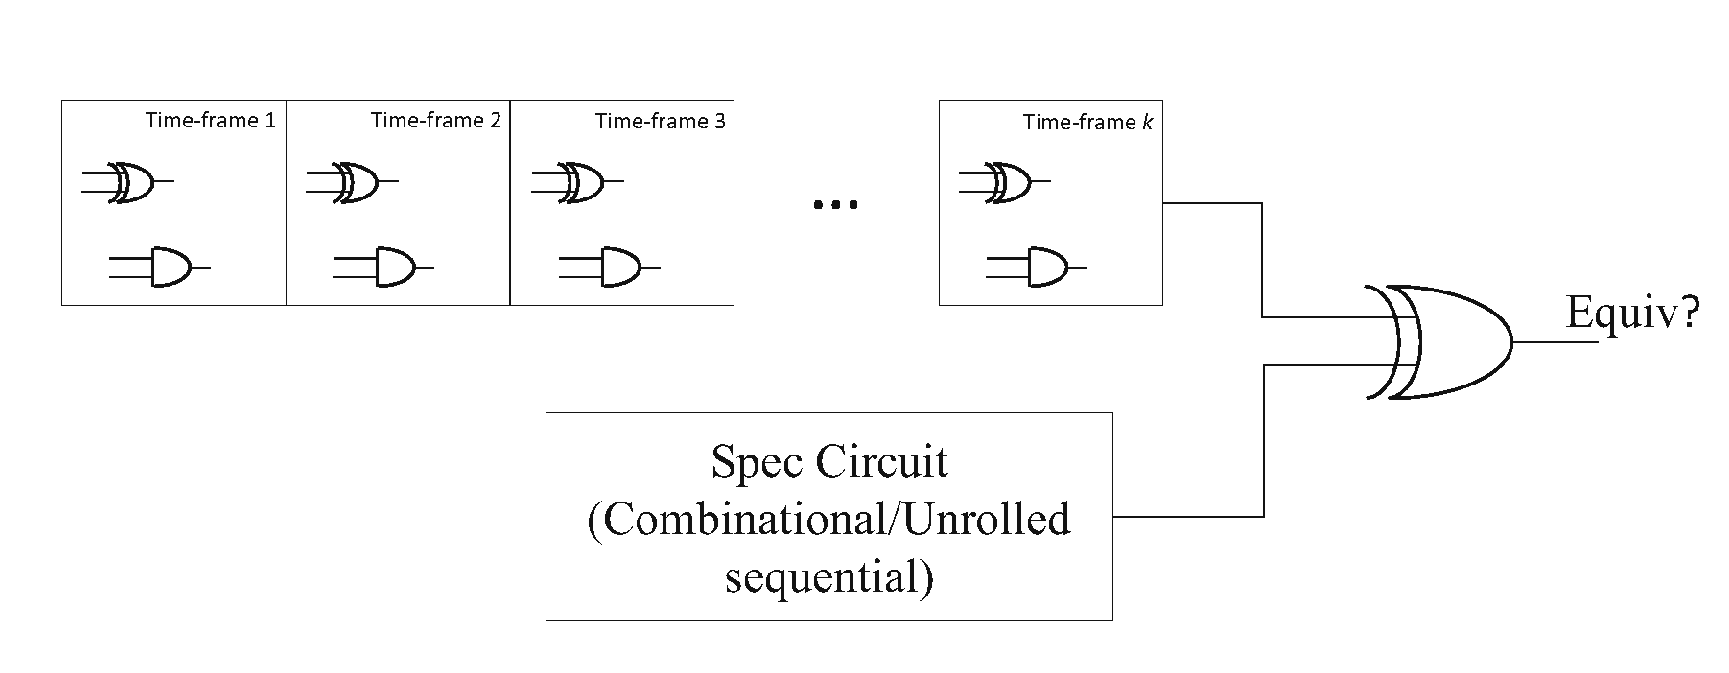
\includegraphics[width=5in]{newfig/convention.eps}
\caption{Conventional verification techniques based on bit-level unrolling and equivalence checking}
\label{fig:convention}}
\end{figure}

Conventional methods to such a sequential circuit may consist of unrolling the circuit for 
$k$ time-frames, and performing an equivalence checking between the unrolled machine and
the specification function. However, the number of gates will grow fast when doing unrolling
on bit-level. Meanwhile the structural similarity based equivalence checking techniques 
will fail when the sequential circuit is highly customized and optimized from the naive specification 
function. As a result, conventional techniques is grossly inefficient for large circuits.
Therefore, a new method based on our proposed word-level FSM traversal technique is worthy to be explored.

\section{Normal Basis Multiplier over Galois Field}
\subsection{Normal Basis}
Given a Galois field (GF) $\Fkk$ is a finite field with  $2^k$ elements and characteristic equals to 2.
Its elements can be written in polynomials of $\alpha$, when there is an irreducible polynomial $p(\alpha)$
defined.

If we use a basis $\{1,\alpha,\alpha^2,\alpha^3,\dots,\alpha^{k-1}\}$, we can easily transform polynomial representations
to binary bit-vector representations by recording the coefficients. For example,

\begin{table}[H]
\centering
\caption{Bit-vector, Exponential and Polynomial representation of
elements in  ${\mathbb{F}}_{2^4} = {\mathbb{F}}_2[x]
\pmod{x^4+x^3+1}$}
\begin{tabular}{|c|c||c|c|} 
\hline
$a_3a_2a_1a_0$ & Polynomial     &$a_3a_2a_1a_0$ & Polynomial  \\
\hline
$0000$        & $0$           & $1000$  &$\alpha^3$\\
\hline
$0001$        & $1$           & $1001$  & $\alpha^3 + 1$\\
\hline
$0010$        &  $\alpha$       & $1010$ & $\alpha^3 + \alpha$  \\
\hline
$0011$        &  $\alpha + 1$   & $1011$ &  $\alpha^3+\alpha+1$\\
\hline
$0100$        &  $\alpha^2$     &  $1100$ &  $\alpha^3 + \alpha^2$\\
\hline
$0101$        & $\alpha^2 + 1$ & $1101$  & $\alpha^3+\alpha^2+1$\\
\hline
$0110$        &  $\alpha^2 + \alpha$ & $1110$ &  $\alpha^3+\alpha^2+\alpha$\\
\hline
$0111$        & $\alpha^2+\alpha+1$ & $1111$ & $\alpha^3+\alpha^2+\alpha+1$\\
\hline
\end{tabular}
\label{table:booltogalois}  
\end{table}

Basis $\{1,\alpha,\alpha^2,\alpha^3,\dots,\alpha^{k-1}\}$ is called {\bf standard basis} (StdB), which results in
a straightforward representation for elements, and operations of elements such as addition and subtraction.
The addition/subtraction of GF elements in StdB follows the rules of polynomial addition/subtraction
where coefficients belong to $\mathbb F_2$. In other words, using the definition of {\it exclusive or} in
Boolean algebra, element $A$ add/subtract by element $B$ in StdB is defined as
\begin{align}\label{eqn:StdB}
A+B = A-B &= (a_0,a_1,\dots,a_{k-1})_{StdB} \xor (b_0,b_1,\dots,b_{k-1})_{StdB} \nonumber\\
&=(a_0\oplus b_0, a_1\oplus b_1,\dots,a_{k-1}\oplus b_{k-1})_{StdB} 
\end{align}

\subsection{Multiplication using Normal Basis}
Besides addition/subtraction, multiplication is also very common in arithmetic circuit design.
The multiplication of GF elements in $\Fkk$ in StdB follows the rule of polynomial multiplication.
However, it will result in $O(k^2)$ bitwise operations. In other words, if we implement GF multiplication
in bit-level logic circuit, it will contain $O(k^2)$ gates. When the datapath size $k$ is large,
the area and delay of circuit will be costly.

In order to lower down the complexity of arithmetic circuit design, Massey and Omura \cite{MasseyOmura} % ref 7 in RH paper
use a new basis to represent GF elements, which is called {\bf normal basis} (NB).
A normal basis over $\Fkk$ is written in the form of
\begin{equation*}
N.B. ~~~ \N = \{\beta,\beta^2,\beta^4,\beta^8,\dots,\beta^{2^{k-1}}\}
\end{equation*}
Respectively, a field element in NB representation is actually
\begin{align*}
A &= (a_0,a_1,\dots,a_{k-1})_{NB} \\
  &= a_0\beta+a_1\beta^2+\cdots+a_{k-1}\beta^{2^{k-1}} \\
  &= \sum_{i=0}^{k-1} a_i\beta^{2^i}
\end{align*}

According to the definition, a normal basis is a vector where the next entry is the square of the former one.
We note that the vector is cyclic, i.e. $\beta^{2^k} = \beta$ due to {\it Fermat's little theorem}.
{\bf Normal element} $\beta$ is an element from the field which is used to construct the normal basis,
and can be represent as a power of primitive element $\alpha$: 
\begin{equation*}
\beta = \alpha^t, ~~~ 1\leq t<2^k
\end{equation*}

The addition and subtraction of elements in NB representation are similar to equation \ref{eqn:StdB}.
However, what makes NB powerful is its property when doing multiplications and exponentiations.
The following lemmas and examples illustrate this fabulous property very well.
\begin{Lemma}[Square of NB]
\label{lem:squareNB}
In $\Fkk$, equation 
\begin{equation*}
(a+b)^2 = a^2 + b^2
\end{equation*}
has been proved. According to the \textbf{binomial theorem}, it can be extended to
\begin{align*}
&(b_0\beta + b_1\beta^2 + b_2\beta^4 + \dots + b_{k-1}\beta^{2^{k-1}})^2 \\
&= b_0^2\beta^2 + b_1^2\beta^4 + b_2^2\beta^8 + \dots + b_{k-1}^2\beta \\
&= b_{k-1}^2\beta + b_0\beta^2 + b_1\beta^4 + \dots + b_{k-2}\beta^{2^{k-1}}
\end{align*}
\end{Lemma}
This lemma concludes that the square of an element in NB equals to a simple right-cyclic shift of the bit-vector.
Obviously, StdB representation does not have this benefit.

\begin{Example}[Square of NB]
In GF $\mathbb F_{2^3}$ constructed by irreducible polynomial $x^3 + x + 1$, the standard basis is denoted as 
$\{ 1, \alpha, \alpha^2\}$ where $\alpha^3+\alpha+1=0$.
Let $\beta = \alpha^3$, then $\N = \{ \beta, \beta^2, \beta^4\}$ forms a normal basis. 
Write down element $E$ using both representations:
\begin{align*}
E &= (a_0,a_1,a_2)_{StdB} = (b_0,b_1,b_2)_{NB} \\
  &= a_0 + a_1\alpha + a_2\alpha^2 = b_0\beta + b_1\beta^2 + b_2\beta^4
\end{align*}
Compute the square of $E$ in StdB first:
\begin{align*}
E^2 &= a_0 + a_1\alpha^2 + a_2\alpha^4 \\
    &= a_0 + a_2\alpha + (a_1 + a_2)\alpha^2 \\
    &= (a_0,a_2,a_1+a_2)_{StdB}
\end{align*}
When it is computed in NB, we can make it very simple:
\begin{align*}
E^2 &= \overset{\xrightarrow{Cyclic~~shift}}{(b_0,b_1,b_2)}_{NB} \\
	&= (b_2,b_0,b_1)_{NB}
\end{align*}
\end{Example}

This example shows that convenience to use NB when computing $2^k$ power of an element.
Multiplication is a bit complicated than squaring; but when it is decomposed as bit-wise
operations, the property in lemma \ref{lem:squareNB} can be well utilized.

\begin{Example}[Bit-wise NB multiplication]
Assume there are 2 binary vectors representing 2 operands in NB over $\Fkk$: 
$A = (a_0, a_1, \dots, a_{k-1}), B = (b_0, b_1, \dots, b_{k-1})$. Note that in this example, 
by default we use normal basis representation so subscript ``NB" is skipped. Their product can also be written
as: $$C = A\times B = (c_0, c_1, \dots, c_{k-1})$$

Assume the most significant bit (MSB) of the product can be represented by a function $f_{mult}$: 
\begin{equation}
\label{eqn:multiMSB}
c_{n-1} = f_{mult}(a_0, a_1, \dots, a_{n-1}; b_0, b_1, \dots, b_{n-1})
\end{equation}
Before discussing the details of the function $f_{mult}$, we can take 
a square on both side of equation \ref{eqn:multiMSB}, i.e. $C^2 = A^2\times B^2$.
Obviously, using the property in lemma \ref{lem:squareNB}, the original second most significant bit 
becomes the new MSB because of right-cyclic shifting. 
Concretely, 
$$(c_{k-1},c_0,c_1,\dots,c_{k-2}) = (a_{k-1},a_0,a_1,\dots,a_{k-2})\times(b_{k-1},b_0,b_1,\dots,b_{k-2})$$
Note $A^2, B^2$ and $C^2$ still belong to $\Fkk$, thus as a universal function implementing MSB multiplication
over $\Fkk$, $f_{mult}$ still keeps the same. As a result, the new MSB can be written as 
\begin{equation}
\label{eqn:shiftMSB}
c_{k-2} = f_{mult}(a_{k-1}, a_0, a_1, 
\dots, a_{k-2}; b_{k-1}, b_0, b_1, \dots, b_{k-2})
\end{equation}
Similarly, if we take a square again on the new equation, we can get $c_{k-3}$.
Successively we can derive all bits of product $C$ using the same function $f_{mult}$, and the only
adjustment we need to make is to right-cyclic shift 2 operands by 1 bit each time.
\end{Example}

From above example, it is proved that a universal structure that implements $f_{mult}$ can be reused
for $k$ times in NB multiplication over $\Fkk$. Comparing to StdB, which requires distinct design 
for every bit of multiplication, NB is less costly if we can prove $f_{mult}$ will not result in 
a structure with $O(k^2)$ complexity. So our next mission is to explore the details of $f_{mult}$
to prove it will be a relatively simple design with complexity lower than $O(k^2)$.

If we want to make the complexity of $f_{mult}$ lower than $O(k^2)$, then the best choice is to try out 
linear functions. As we know, matrix multiplication can simulate all possible combinations of 
linear functions (which is also the reason it is used as basic model to simulate the behavior of a neuron
in neural network machine learning algorithms). Imagine $A$ is a $k$-bit row vector and $B$ is a $k$-bit 
column vector, then the single bit product can be written as the product of matrix multiplication
$$c_{l} = A\times C\times B$$
where $C$ is a $k\times k$ square matrix.

\begin{Definition}[$\lambda$-Matrix]
A binary $k\times k$ matrix $M$ is used to describe the bit-wise normal basis multiplication function $f_{mult}$ where
\begin{equation}
\label{eqn:def_lambda}
c_{l} = f_{mult}(A, B) = A \times M \times B^T
\end{equation}
$B^T$ denotes vector transposition. Matrix $M$ is called $\lambda$-Matrix of
$k$-bit NB multiplication over $\Fkk$.
\end{Definition} 

When taking different bits $l$ of the product in equation \ref{eqn:def_lambda}, 
we obtain a series of conjugate matrices of $M$. 
Which means instead of shifting operands $A$ and $B$, we can also shift the 
matrix.

More specifically, we denote the matrix by \emph{$l$-th $\lambda$-Matrix} as 
$$c_l = A \times M^{(l)} \cdot B^T$$
Meanwhile, the operator shifting rule in equation \ref{eqn:shiftMSB} still holds. Then we have relation 
$$c_{l-1} = A \cdot M^{(l-1)} \cdot B^T = shift(A) \cdot M^{(l)} \cdot shift(B)^T$$ which means
by right and down cyclically shifting $M^{(l-1)}$, we can get $M^{(l)}$.

\begin{Example}[NB multiplication using $\lambda$-Matrix]
Over GF $\mathbb F_{2^3}$ constructed by irreducible polynomial $\alpha^3 + \alpha + 1$, let normal element $\beta = \alpha^3$, $N = \{ \beta, \beta^2, \beta^4\}$ 
forms a normal basis. Corresponding $0$-th $\lambda$-Matrix is
\begin{equation*}
M^{(0)} = \left(
\begin{array} {lcr}
0 & 1 & 0\\
1 & 0 & 1\\
0 & 1 & 1
\end{array} \right).
\end{equation*}
i.e.,
\begin{equation*}
c_0 = (a_0\  a_1\  a_2)\left(
\begin{array} {lcr}
0 & 1 & 0\\
1 & 0 & 1\\
0 & 1 & 1
\end{array} \right)\left(
\begin{array} {lcr}
b_0\\
b_1\\
b_2
\end{array} \right)
\end{equation*}
From $0$-th $\lambda$-Matrix we can directly write down all remaining $\lambda$-Matrices:
\begin{equation*}
M^{(1)} = \left(
\begin{array} {lcr}
1 & 0 & 1\\
0 & 0 & 1\\
1 & 1 & 0
\end{array} \right)~~~~~~
M^{(2)} = \left(
\begin{array} {lcr}
0 & 1 & 1\\
1 & 1 & 0\\
1 & 0 & 0
\end{array} \right)
\end{equation*}
\end{Example}

If we generalize the definition and explore the nature of $\lambda$-Matrix, it is defined as cross-product terms from multiplication, which is 
\begin{equation}
Product~vector~C = (\sum_{i=0}^{k-1}a_i\beta^{2^i})(\sum_{j=0}^{k-1}b_j\beta^{2^j}) = \sum_{i=0}^{k-1}\sum_{j=0}^{k-1}a_ib_j\beta^{2^i}\beta^{2^j}
\end{equation}
The expressions $\beta^{2^i}\beta^{2^j}$ are referred to as cross-product terms, and can be represented by
NB, i.e.
\begin{equation}
\beta^{2^i}\beta^{2^j} = \sum_{l=0}^{k-1}\lambda_{ij}^{(l)}\beta^{2^l}, \ \ \lambda_{ij}^{(l)} \in \mathbb F_2.
\end{equation}
Substitution yields, result is an expression for l-th digit of product as showed in equation \ref{eqn:multiMSB}:
\begin{equation}
c_l = \sum_{i=0}^{k-1}\sum_{j=0}^{k-1}\lambda_{ij}^{(l)}a_ib_j
\end{equation}
$\lambda_{ij}^{(l)}$ is the entry with coordinate $(i,j)$ in $l$-th $\lambda$-Matrix.

The $\lambda$-Matrix can be implemented with XOR and AND gates in circuit design.
The very naive implementation requires $O(C_N)$ gates, where $C_N$ is the number of
nonzero entries in $\lambda$-Matrix.
There usually exists multiple NBs in $\Fkk, k>3$. If we employ a random NB, there is no mathematical
guarantee that $C_N \sim o(k)$ (symbol $o$ denotes ``strictly lower than bound"). However,
Mullin et al. \cite{mullinONB} % This citation is valid
proves that in certain GF $\mathbb F_{p^{k_{opt}}}$, there always exists at least one NB such that 
its corresponding $\lambda$-Matrix has $C_N = 2n-1$ nonzero entries. A basis with this property is
called optimal normal basis (ONB), details are introduced in appendix.

In practice, large size NB multipliers are usually designed in $\Fkk$ when ONB exists
to minimized the number of gates. So in the following part of this chapter and our experiments,
we only focus on ONB multipliers instead of general NB multipliers.


% After fixing this, add a whole-piece StdB vs NB example, list their cost as the conclusion
\subsection{Comparison between Standard Basis and Normal Basis}
At the end of this section, a detailed example is used to make a comparison between StdB multiplication
and NB multiplication.
\begin{Example}[Rijndael's finite field]
Rijndael uses a characteristic 2 finite field with 256 elements, which can also be called the GF $\mathbb F_{2^8}$.
Let us define the primitive element $\alpha$ using irreducible polynomial 
$\alpha^8+\alpha^7+\alpha^6+\alpha^4+\alpha^2+\alpha+1$. Coincidently, $\alpha$ is also a normal element,
i.e. $\beta = \alpha$ can construct a NB $\{\alpha,\alpha^2,\alpha^4,\alpha^8,\alpha^{16},\alpha^{32},\alpha^{64},
\alpha^{128}\}$.

We pick a pair of elements from the Rijndael's field: $A=(0100~1011)_{StdB} = (4B)_{StdB},~B=(1100~1010)_{StdB} = (CA)_{StdB}$.
First let us compute their product in StdB, the rule follows ordinary polynomial multiplication.

\begin{align*}
A\cdot B &= (\alpha^6+\alpha^3+\alpha+1)(\alpha^7+\alpha^6+\alpha^3+\alpha)\\
&= (\alpha^{13}+\alpha^{10}+\alpha^8+\alpha^7)+(\alpha^{12}+\alpha^9+\alpha^7+\alpha^6)+
	(\alpha^9+\alpha^6+\alpha^4+\alpha^3)\\
	&~~~+(\alpha^7+\alpha^4+\alpha^2+\alpha) \\
&= \alpha^{13}+\alpha^{12}+\alpha^{10}+\alpha^8+\alpha^7+\alpha^3+\alpha^2+\alpha
\end{align*}
Note that this polynomial is not the final form of the product because it needs to be
reduced modulo irreducible polynomial $\alpha^8+\alpha^7+\alpha^6+\alpha^4+\alpha^2+\alpha+1$.
This can be done using base-2 long division. Note the dividend and divisor are written in pseudo Boolean
vectors, not real Boolean vectors in any kind of bases.

% The folowing part is customized latex code mimicing binary long division
% Note \divrule coordinates may not reflect the intuitive column # in tabular. Adjust by urself!!!

\vspace{1cm}

\newdimen\digitwidth
\settowidth\digitwidth{0}
\def~{\hspace{\digitwidth}}


\def\divrule#1#2{%
\noalign{\moveright#1\digitwidth%
\vbox{\hrule width#2\digitwidth}}}
111010111\,\begin{tabular}[b]{@{}r@{}}
101001 \\ \hline
\big)\begin{tabular}[t]{@{}l@{}}
11010110001110 \\
111010111 \\ \divrule{0}{14}
~~111101101 \\
~~111010111 \\ \divrule{2}{12}
~~~~~111010110 \\
~~~~~111010111 \\ \divrule{5}{9}
~~~~~~~~~~~~~1
\end{tabular}
\end{tabular}
\vspace{0.5cm}

The final remainder is $1$, i.e. the product equals to 1 in StdB.

On the other hand, operands $A$ and $B$ can be written in NB as
$$A = (0010~1001)_{NB},~~B = (0100~0010)_{NB}$$
The $\lambda$-Matrix for $\mathbb F_{2}[x] \pmod{x^8+x^7+x^6+x^4+x^2+x+1}$
is
(Computation of $\lambda$-Matrix refers to appendix)
\begin{equation*}
M^{(0)} = \left(\begin{array}{lccccccr}
0 &0 &0 &0 &1 &0 &1 &1 \\
0 &0 &1 &1 &1 &1 &0 &0 \\
0 &1 &0 &0 &0 &0 &1 &0 \\
0 &1 &0 &0 &1 &1 &0 &1 \\
1 &1 &0 &1 &0 &1 &0 &0 \\
0 &1 &0 &1 &1 &0 &0 &1 \\
1 &0 &1 &0 &0 &0 &0 &0 \\
1 &0 &0 &1 &0 &1 &0 &1
\end{array}\right)
\end{equation*}
Taking matrix multiplication $c_0 = A\times M^{(0)}\times B^T$,
the result is $c_0 = 1$. Then by cyclic shifting $A$ and $B$
(or shifting $M^{(0)}$, either is applicable), we can successively
obtain other bits of product. The final answer is
$$C = (0000~0001)_{NB}$$
It is equivalent to the result in StdB.
\end{Example}

From the intuition of humans, StdB multiplication is straightforward and easier to understand
while NB is difficult to comprehend. However, if we implement both multiplications to 
hardware multipliers, it will be clear which side a circuit designer prefers.

% May consider providing details?

Mastrovito multiplier and Montgomery multiplier are 2 common designs
of GF multipliers using StdB. As a naive implementation of GF multiplication,
Mastrovito multiplier uses most number of gates:
$k^2$ AND gates plus $k^2-\Delta$ XOR gates \cite{Mastrovito}. Montgomery multiplier 
applies lazy reduction techniques and results in a better latency performance, while the number of gates are about
the same with Mastrovito multiplier:
$k^2$ AND gates plus $k^2-k/2$ XOR gates \cite{Montgomery}. 
Concretely, typical design of Mastrovito multiplier consists of 218 logic gates, while 
Montgomery multiplier needs 198 gates. However, the NB multiplier reuses the $\lambda$-Matrix 
logic, so this component will only need to be implemented for once. 
Consider the definition of matrix multiplication, it needs $C_N$ AND gates to apply 
bit-wise multiplication and $C_N-1$ XOR gates to sum them up. The number of nonzero entries
in the $\lambda$-Matrix can be counted: $C_N = 27$.
As a result, the most naive NB multiplier design (or Massey-Omura multiplier \cite{MasseyOmura})
contains 53 gates in total, which is a great saving in area cost comparing to StdB multipliers.
\chapter{Finding Unsatisfiable Cores Extraction for a Set of Polynomials using the Gr\"obner Basis Algorithm}
\label{ch:UNSAT}
Besides elimination ideal based abstraction, Gr\"obner basis can also be applied to a vast field
about other techniques in formal verification. Satisfiability (SAT) problem is the basis of modern 
computation theories, as well as the origin of most formal verification problem. 
In this chapter, we will discuss a sort of problems branching out from SAT. They are about a situation 
when SAT problems give negative answer, which are called unsatisfiability (UNSAT) problems. Within 
a set of constrains (e.g. clauses, formulas or polynomials) which is unsatisfiable, sometimes 
it is worthy to explore a smaller subset (core) that keeps UNSAT. From the execution of GB algorithm, 
an auxiliary structure can be obtained to help UNSAT core extraction. This chapter will introduce the 
details about the motivation, mechanism and implementation. 

\section{Motivation}
\subsection{Exploiting UNSAT cores for abstraction refinement}
By exploring previous work, we learn that most state-of-art abstraction refinement techniques require 
information mining from UNSAT proofs of intermediate abstractions. 
Here we use an abstraction refinement algorithm from \cite{zhang2005design} to explain that how an UNSAT proof is
utilized in such techniques.

\begin{algorithm}[hbt]
\SetAlgoNoLine
	\KwIn{$M$ is the original machine, $p$ is the property to check, $k$ is the number of steps in $k$-BMC}
  $k = $ InitValue\;
  \eIf{$k$-BMC$(M,p,k)$ is \textbf{SAT}}
  {
	\Return{``Found error trace"}
  }
  {
	Extract UNSAT proof $\mathcal P$ of $k$-BMC\;
	$M' = $ \textit{ABSTRACT}$(M,\mathcal P)$\;
  }
  \eIf{MODEL-CHECK$(M',p)$ returns \textbf{PASS}}
  {
	\Return{``Passing property"}
  }
  {
	Increase bound $k$\;
	goto Line 2\;
  }
\caption {Abstraction refinement using $k$-BMC}\label{alg:absrefine}
\end{algorithm}
\begin{figure}[hbt]
\centering{
\includegraphics[width=5.5in]{newfig/refine.eps}
\caption{Abstraction by reducing latches}
\label{fig:refine}}
\end{figure}
Assume that we are given a sequential circuit with $n$ latches as shown in Fig.\ref{fig:refine}(a). 
This circuit can be modeled as a Mealy machine $M$ and the states $s$ can be explicitly encoded by bit-level latch variables 
$l_1,\dots,l_n$. Algorithm \ref{alg:absrefine} describes an approach to check if machine $M$ violates property $p$.
This algorithm relies on $k$-BMC technique, which works on the basis of CNF-SAT solving.
The $k$-BMC represents the initial states $I$, the transition relation $T$ and property $p$ as CNF formulas.

The first ``if-else" branch in Algorithm \ref{alg:absrefine} can be
explained as: we check if the conjunction of formulas 
$$I(s_0)\land \bigwedge_{i=0}^{k-1}T(s_i,s_{i+1}) \land \neg p$$
is $SAT$ or not, where $s_i$ denotes the set of reached states in $i$-th time-frame. If the result is
$SAT$, then a counterexample is found that violates property $p$. If the result is $UNSAT$, we cannot
assert that $p$ is satisfied for the original machine $M$ because we only unrolled $M$ for a given specific number of time-frames
without any fixpoint detected.
In this algorithm, we analyze the UNSAT core composed by a set of clauses whose conjunction is $UNSAT$.
If there are some latch variables not included in this UNSAT core (denoted by $L_{abs}$), then we can assert that the evaluations of 
these variables will not affect the unsatisfiability of original formula. Therefore, we can ignore them in the abstracted model.
In practice, we turn these latches into primary inputs/outputs as shown in Fig.\ref{fig:refine}(b) ($L_{abs} = \{l_1,\dots,l_m\}$).


The second ``if-else" branch means: if we do an ordinary model checking on the abstracted machine $M'$ and find no
error trace, we can assert that property $p$ also holds on the original machine $M$. The reason of this assertion is that
the abstracted states represented using abstracted latches cover the original states, which means $M'$ is an over-approximation
of $M$, such that $(M'\implies p) \implies (M\implies p)$. If we find a violation on abstracted machine, then this
abstracted model is not a suitable model to check $p$, so we have to increase the bound $k$ to find a finer abstraction.

It is clear that UNSAT cores play an important role in abstraction refinement approaches. In \cite{zhang2005design}
the UNSAT core is extracted using a conventional CNF-SAT solver, which will encounter the ``bit-blasting" problem
when the size of datapath (number of latches in Fig.\ref{fig:refine}) is very large. \textbf{Here we propose a totally new 
method based on Gr\"obner basis computation to extract UNSAT cores, and we believe it may become an efficient 
method according to the following observation based on our experience:}

% {\it Gr\"obner basis is more suitable for UNSAT problems because of following theorem:}
{\it While computing GB over finite fields is exponential in the number of variables, GB  computation 
is observed to be more efficient for UNSAT problems.} 
The reason is discussed as follows:
\begin{Theorem}
{\bf Weak Nullstellensatz:} Given ideal $J\subset \mathbb F[x_1,\dots,x_n]$, its variety over algebraic closure
of field $\mathbb F$ is empty if and only if its reduced Gr\"obner basis contains only one generator ``1".
$${\bf V}_{\overline{\mathbb F}}(J) = \emptyset \Longleftrightarrow reducedGB(J) = \{1\}$$
\end{Theorem}
It is well known that using Buchberger's algorithm and its variations to compute a GB has a very high
time complexity and is usually not practicable. One reason is that the size of GB may explode even if the term
ordering is carefully chosen. However if the reduced GB is 1, which means every term in the original polynomials
will be canceled, the degree of remainders when computing GB with Buchberger's algorithm will be limited. 
Thus the number of polynomials in non-reduced GB is much smaller than usual.
Instead of applying polynomial calculus to SAT solving, it may be more efficient to try it for UNSAT
problems.

\subsection{A Demonstration of Motivating Example}
One  important research topic about UNSAT problems is to identify UNSAT cores efficiently.
An UNSAT core in a CNF formula denotes a subset of clauses which is still unsatisfiable. Here
we re-define this concept in algebraic geometry:
\begin{Definition}
Assume a set of polynomials $F$ and its subset $F_s\subset F$. If ${\bf V}(\langle F\rangle) = {\bf V}
(\langle F_s\rangle) = \emptyset$, we call $F_s$ an {\bf UNSAT core} of $F$. Additionally, if
$F_s$ contains no other UNSAT core, we call it a {\bf minimal} UNSAT core.
\end{Definition}

We  conjecture that based on observation of Buchberger's algorithm's execution, an UNSAT core can be identified.
\begin{Proposition}
Buchberger's algorithm picks pairs of polynomials from a given set, computes their S-poly, then reduces this S-poly
with the given set of polynomials. If the remainder is non-zero,
it is added to the set of polynomials.
By tracking S-poly computations and multivariate divisions that lead to remainder 
1, we can obtain an UNSAT core. Moreover, we can identify a minimal UNSAT core with one-time
 execution of Buchberger's algorithm.
\end{Proposition}
\begin{Example}
A SAT problem is described with 8 CNF clauses:

\begin{minipage}[h]{0.3\textwidth}
\begin{align*}
&c_1: \bar{a}\lor\bar{b}\\
&c_2: a\lor\bar{b}\\
&c_3: \bar{a}\lor b\\
&c_4: a\lor b
\end{align*}
\end{minipage}
\begin{minipage}[h]{0.7\textwidth}
\begin{align*}
&c_5: x\lor y\\
&c_6: y\lor z\\
&c_7: b\lor \neg y\\
&c_8: a\lor x\lor \neg z
\end{align*}
\end{minipage}

% \begin{align*}
% &\bar{a}\lor\bar{b}\\
% &a\lor\bar{b}\\
% &\bar{a}\lor b\\
% &a\lor b\\
% &x\lor y\\
% &y\lor z\\
% &b\lor \neg y\\
% &a\lor x\lor \neg z
% \end{align*}
Using Boolean to polynomial mappings given in Table \ref{tab:booltof4}, we can transform them to a set of
polynomials $F$ over ring $\mathbb F_2[a,b,x,y,z]$:

\begin{minipage}[h]{0.4\textwidth}
\begin{align*}
&f_1:ab\\
&f_2:ab+a\\
&f_3:ab+b\\
&f_4:ab+a+b+1
\end{align*}
\end{minipage}
\begin{minipage}[h]{0.6\textwidth}
\begin{align*}
&f_5:xy+y+x+1\\
&f_6:yz+y+z+1\\
&f_7:by+y\\
&f_8:axz+az+xz+z
\end{align*}
\end{minipage}
% \begin{align*}
% &f_1:ab\\
% &f_2:ab+a\\
% &f_3:ab+b\\
% &f_4:ab+a+b+1\\
% &f_5:xy+y+x+1\\
% &f_6:yz+y+z+1\\
% &f_7:by+y\\
% &f_8:axz+az+xz+z
% \end{align*}
We compute its GB using Buchberger's algorithm with lexicographic term ordering $a>b>x>y>z$.
Since this problem is UNSAT, we will stop when ``1" is added to GB.
\begin{enumerate}
\item First we compute $Spoly(f_1,f_2)\xrightarrow{F}_{+} r_1$, remainder $r_1$ equals to $a$;
\item Update $F=F\cup r_1$;
\item Next we compute $Spoly(f_1,f_3)\xrightarrow{F}_{+} r_2$, remainder $r_2$ equals to $b$;
\item Update $F=F\cup r_2$;
\item We can use a directed acyclic graph (DAG) to represent the process to get $r_1,r_2$, as Fig.\ref{fig:UNSAT}(a) shows;
\item Then we compute $Spoly(f_1,f_4) = s_3= a+b+1$, obviously $a+b+1$ can be reduced (multivariate divided) by
$r_1$ , the intermediate remainder $r_3 = b+1$. It can be immediately divided by $r_2$, and the remainder is ``1", we
terminate the Buchberger's algorithm;
\item We draw a DAG depicting the process through which we obtain remainder ``1" as shown in Fig.\ref{fig:UNSAT}(b). 
From leaf ``1" we backtrace the graph to roots $f_1,f_2,f_3,f_4$. They constitute an UNSAT core for this problem
as these polynomials are the ``causes" of unsatisfiability of original set of clauses.
\end{enumerate}
\end{Example}
\begin{figure}[hbt]
\centering{
\includegraphics[width=\textwidth]{newfig/UNSAT.eps}
\caption{DAG representing Spoly computations and multivariate divisions}
\label{fig:UNSAT}}
\end{figure}
% We conclude our approach as follows: i) Keep track of all $Spoly(f_i,
% f_j)\xrightarrow{f_1, \dots, f_s}_+ r$; ii) mark $f_i, f_j$ if $r\neq
% 0$; iii) Mark those $f_l$'s that have leading terms that cancel
% monomial terms in $Spoly(f_i, f_j)$; iv) Build a DAG recording all reductions including Spoly computations
% and multivariate divisions; v) Once $1\in J$ is
% detected, traverse the graph to identify all the marked polynomials that were
% used in obtaining this unit element. These polynomials constitute the
% core.

We conclude our approach as a conjecture algorithm (Algorithm \ref{alg:UNSAT}). 

\begin{algorithm}[hbt]
\SetAlgoNoLine
	\KwIn{A set of polynomials $F = \{f_1,f_2,\dots,f_s\}$}
	\KwOut{An UNSAT core $\{f_{m_1},f_{m_2},\dots,f_{m_t}\}$}
\Repeat{$r_l == 1$}
{
	Pick a pair $f_i,f_j\in F$ that has never been computed S-poly\;
	\If{$Spoly(f_i,f_j)\xrightarrow{F}_+ r_l \neq 0$}
	{
		$F = F\cup r_l$\;
		Create a DAG $G_l$ with $f_i,f_j$ as roots, $r_l$ as leaf, recording the S-poly, all intermediate remainders and $f_k\in F$ that cancel monomial terms in the S-poly\;
	}
}
Backward traverse the DAG for remainder ``1", replace $r_l$ with corresponding DAG $G_l$\;
\Return{All roots}
\caption {Extract UNSAT core using a variation of Buchberger's algorithm}\label{alg:UNSAT}
\end{algorithm}

\section{Formalize the Buchberger's Algorithm based UNSAT Core Identification}
\label{sec:core}

\textbf{Problem: }
Let $F = \{f_1, \dots f_s\}$ be a set of multivariate polynomials in
the ring $R = \F[x_1,\dots,x_d]$ that generate ideal $J = \langle
f_1,\dots,f_s\rangle \subset R$. Suppose that it is known that $V(J) =
\emptyset$, or it is determined to be so by applying the Gr\"obner
basis algorithm. Identify a subset of polynomials $F_c \subseteq F,
J_c = \langle F_c \rangle$, such that $V(J_c) = \emptyset$
too. Borrowing the terminology from the Boolean SAT domain, we
call $F_c$ the infeasible core or the unsat core of $F$. 

%% Any set of polynomials $F$ with empty variety is an unsat core in
%% itself. There may be more than one unsat cores in $F$, some
%% polynomials may be common to multiple cores (i.e. the
%% cores may be non-disjoint), and these cores may have
%% different cardinalities $|F_c|$. The unsat core problems
%% are therefore further classified as: 
%% \bi
%% \item Identify a {\it minimum} core, i.e. a core of minimum
%%   cardinality. 
%% \item Identify a {\it minimal} core. An unsat core $F_{c}$ is minimal
%%   with respect to the property that while the variety of $F_{c}$ is
%%   empty, the variety of {\it any} subset of $F_c$ is {\it non-empty},
%%   i.e. $V( F_{c} - \{f_i\} ) \neq \emptyset$ for any $f_i \in
%%   F_c$. 
%% \item Identify any unsat core disregarding minimality; i.e. find any
%%   subset $F_c$ of $F$.
%% \ei

%% Let us first consider the problem of finding any $F_c \subset F$,
%% disregarding minimality. 
It is not hard to motivate that an unsat core should be identifiable
using the Gr\"obner basis algorithm: Assume that $F_c=F-\{f_j\}$. If
$GB(F) = GB(F_c) = \{1\}$, then it implies that $f_j$ is a member of
the ideal generated by $(F - \{f_j\})$, i.e. $f_j \in \langle F -
\{f_j\}\rangle$. Thus $f_j$ can be composed of the other
polynomials of $F_c$, so $f_j$ is  not a part of the unsat core, and
it can be safely discarded from $F_c$. This can be identified by means
of the GB algorithm for this ideal membership test.% (Def. \ref{def:gb}(ii)).  

A n\"aive way (and inefficient way) to identify {\it a minimal core}
using the GB computation is as follows:
select a polynomial $f_i$ and see if $V(F_c - \{f_i\}) = \emptyset$
(i.e. if reduced $GB(F_c - \{f_i\}) = \{1\}$). If so, discard $f_i$
from the core; otherwise retain $f_i$ in $F_c$. Select a different
$f_i$ and continue until all polynomials $f_i$ are visited for
inclusion in $F_c$. This approach will produce a minimal core, as we
would have tested each polynomial $f_i$ for inclusion in the
core. This requires $O(|F|)$ calls to the GB engine, which is really
impractical.   

\subsection{The Refutation Tree of the GB Algorithm: Find $F_c$ from $F$}

We investigate if it is possible to identify a core by analyzing the
$Spoly(f_i,f_j)\xrightarrow{F}_+ g_{ij}$ reductions in Buchberger's
algorithm. Since $F$ is itself an unsat core, 
definitely {\it there exists  
a sequence of Spoly reductions in Buchberger's algorithm where
$Spoly(f_i, f_j) \xrightarrow{F}_+ 1$ is achieved.} Moreover, 
polynomial reduction algorithms can be suitably modified to record
which polynomials from $F$ are used in the division leading to
$Spoly(f_i,f_j)\xrightarrow{F}_+1$. This suggests that 
we should be able to identify a core by recording
the {\it data} generated by Buchberger's algorithm --- namely, the
critical pairs($f_i,f_j$) used in the Spoly computations,
and the polynomials from $F$ used to cancel terms in the reduction
$Spoly(f_i,f_j)\xrightarrow{F}_+1$. The following example motivates
our approach to identify  $F_c \subseteq F$ using this data:

\begin{Example}
\label{ex:1}
Consider the following set of polynomials $F = \{f_1,\dots, f_9\}$:

\begin{minipage}{2in}
\begin{align*}
f_1&: abc + ab + ac + bc \\
   & + a + b + c + 1\\
f_2&: b\\
f_3&: ac\\
f_4&: ac + a
\end{align*}
\end{minipage}
%\hspace{0.1in}
\begin{minipage}{3in}
\begin{align*}
f_5&: bc + c\\
f_6&: abd + ad + bd + d\\
f_7&: cd\\
f_8&: abd + ab + ad + bd + a + b + d + 1\\
f_9&: abd + ab +bd + b
\end{align*}
\end{minipage}



Assume $>_{DEGLEX}$ monomial ordering with $a>b>c>d$. 
Let $F = \{f_1,\dots,f_9\}$ and 
$J = \langle F \rangle \subset \mathbb{F}_2[a,b,c,d]$ where
$\mathbb{F}_2 = \{0, 1\}$ is the finite field of 2 elements. Then 
$V(J) = \emptyset$ as $GB(J) = 1$.  The set $F$ consists of 4 {\it minimal}
cores: $F_{c1} = \{ f_1,f_2,f_3,f_4,f_7,f_8\}, F_{c2} = \{
f_2,f_4,f_5,f_6,f_8\}, F_{c3} = \{ f_2,f_3,f_4,f_6,f_8\},$ and $F_{c4}
= \{ f_1,f_2,f_4,f_5\}$. 
\end{Example}

Buchberger's algorithm terminates to a unique reduced GB, irrespective
of the order in which the critical pairs $(f_i,f_j)$ are selected and reduced by operation
$Spoly(f_i,f_j)\xrightarrow{F}_+g_{ij}$. Let us suppose that in the GB
computation corresponding to Example \ref{ex:1}, the first 3 critical
{\it Spoly} pairs analyzed are $(f_1, f_2), (f_3, f_4)$ and
$(f_2,f_5)$. It turns out that the Spoly-reductions corresponding to
these 3 pairs lead to the unit ideal. Recording the data
corresponding to this sequence of reductions is depicted by means of a
graph in Fig. \ref{fig:refute}. We call this graph a {\it refutation tree}. 


\begin{figure}[hbt]
\centering
\includegraphics[width=\textwidth]{newfig/refutation_tree.eps}
\caption{Generating refutation trees to record unsat cores}
\label{fig:refute}
\end{figure}

In the figure, the nodes of the graph correspond to the polynomials
utilized in Buchberger's algorithm. The leaf nodes always correspond
to polynomials from the given generating set. An edge $e_{ij}$ from
node $i$ to node $j$ signifies that the polynomial at node $j$ results
from polynomial at node $i$. For example, consider the computation
$Spoly(f_1,f_2)\xrightarrow{F}_+ f_{10}$, where $f_{10} = a + c +
1$. Since $Spoly(f_1, f_2) = f_1 - ac\cdot f_2$, the leaves
corresponding to $f_1$ and $ac\cdot f_2$ are created. The reduction
$Spoly(f_1,f_2)\xrightarrow{F}_+ f_{10}$ is carried out as the
following sequence of 1-step divisions:
$Spoly(f_1,f_2)\xrightarrow{a\cdot f_2} ~\xrightarrow{f_3}~
\xrightarrow{c\cdot f_2}  ~\xrightarrow{f_2} f_{10}$. This is depicted
as the bottom subtree in the figure, terminating at polynomial
$f_{10}$. Moreover, the multiplication $a\cdot f_2$ implies that
division by $f_2$ resulted in the quotient $a$. The refutation tree of
Fig. \ref{fig:refute} shows further that
$Spoly(f_3,f_4)\xrightarrow{f_{10}} f_{11} = c+1$ and, finally,
$Spoly(f_5,f_2)\xrightarrow{f_{11}} 1$. 
 
To identify an $F_c \subset F$, we start from the refutation node
``1'', and traverse the graph in reverse, all the way up to the
leaves. Then, all the leaves in the transitive fanin of ``1''
constitute an unsat core. The polynomials (nodes) that do not lie in
the transitive fanin of ``1'' can be safely discarded from $F_c$. From
Fig. \ref{fig:refute}, $F_c = \{f_1,f_2,f_3,f_4,f_5\}$ is identified
as an unsat core of $F$. 

\section{Reducing the Size of the Infeasible Core $F_c$}
\label{sec:alg}
The core $F_c$ obtained from the aforementioned procedure may
contain redundant elements which could be discarded. For
example, consider the core $F_c=\{f_1,\dots, f_5\}$ generated in the
previous section. While $F_c$ is a smaller infeasible core of $F$, it
is not minimal. In fact, Example 1 shows that $F_{c4} =\{f_1,f_2,f_4,f_5\}$ is the
minimal core, where $F_{c4} \subset F_{c}$. Clearly, the polynomial
$f_3 \in F_c$ is a redundant element of the core and can be 
discarded. We will now describe techniques to further reduce the size
of the unsat core by identifying such redundant elements. 
%how the size of this core could be reduced further.  
For this purpose, we will have to perform a more 
systematic book-keeping of the data generated during the execution of
Buchberger's algorithm and the refutation tree. 

\subsection{Identifying redundant polynomials from the refutation tree}

We record the S-polynomial reduction
$Spoly(f_i,f_j)\xrightarrow{F}_+{g_{ij}}$ that give a non-zero
remainder when divided by the system of polynomials $F$ at that
moment. The remainder $g_{ij}$ is a polynomial combination of
$Spoly(f_i,f_j)$ and the current basis $F$; thus, it can be
represented as:
\begin{equation}
\label{eqn1}
g_{ij}= S(f_i,f_j)+\displaystyle\sum_{k=1}^m c_kf_k,
\end{equation}
where $0\neq c_k\in\mathbb{F}[x_1,\ldots,x_d]$ and
$\{f_1,\ldots,f_m\}$ is the ``current'' system of polynomials
$F$. For each non-zero $g_{ij}$, we will record the following data: 

\begin{equation}
\label{data1}
((g_{ij})(f_{i},h_{ij})(f_{j},h_{ji})| (c_{k1},f_{k1}),(c_{k2},f_{k2}),\dots,(c_{kl},f_{kl}))
\end{equation}

In Eqns. (\ref{eqn1}) and (\ref{data1}), $g_{ij}$ denotes the
remainder of the $S$-polynomial $Spoly(f_i,f_j)$ modulo the current system
of polynomials $f_1,\ldots,f_m$, and we denote by  

$$h_{ij}:=\displaystyle\frac{LCM(lm(f_i),lm(f_j))}{lt(f_i)},
h_{ji}:= - \displaystyle\frac{LCM(lm(f_i),lm(f_j))}{lt(f_j)}$$ 
the coefficients of $f_i$, respectively $f_j$, in the $S$-polynomial
$Spoly(f_i,f_j)$. Furthermore, in Eqn. (\ref{data1}), $(c_{k1}, \dots
c_{kl})$ are the respective quotients of division by
polynomials $(f_{k1},\dots,f_{kl})$, generated during the $Spoly$ reduction.  
%polynomial coefficients of  that appear in the
%division process. 

\begin{Example}
Revisiting Ex. \ref{ex:1}, and Fig. \ref{fig:refute}, the data
corresponding to $Spoly(f_1,f_2)$\\$\xrightarrow{F}_+  g_{12} = f_{10}$
reduction is obtained as the following sequence of computations:
$$f_{10}=g_{12}=f_1-acf_2-af_2-f_3-cf_2-f_2.$$ As the coefficient
field is $\mathbb{F}_2$ in this example, $-1 = +1$, so:
$$f_{10}=g_{12}=f_1+acf_2+af_2+f_3+cf_2+f_2$$ is obtained.
The data is recorded according to Eqn. (\ref{data1}):

\begin{center}
$((f_{10}=g_{12}), (f_1,1)(f_2,ac)|(a,f_2),(1,f_3),(c,f_2),(1,f_2))$
\end{center}

\end{Example}

Our approach and the book-keeping terminates when we obtain ``1'' as the
remainder of some S-polynomial modulo the current system of 
generators. As an output of the Buchberger's algorithm, we can obtain
not only the Gr\"obner basis $G = \{g_1,\ldots,g_t\}$, but also a
matrix $M$ of polynomials such that: 

\vspace{-0.1in}
\begin{center}
\begin{align}
   \begin{bmatrix}
           g_{1} \\
           g_{2} \\
           \vdots \\
           g_{t}
         \end{bmatrix}
    &= M \begin{bmatrix}
           f_{1} \\
           f_{2} \\
           \vdots \\
           f_{s}
         \end{bmatrix}
  \end{align}

\end{center}

Each element $g_i$ of $G$ is a polynomial combination of $\{f_1, \dots,
f_s\}$. Moreover, this matrix $M$ is constructed precisely using the
data that is recorded in the form of Eqn. (\ref{data1}). We now give a condition
when the matrix $M$ may identify some redundant elements. 


\begin{Theorem}
\label{thm}
With the notations above, we have that a core for the system of
generators $F = \{f_1,\dots,f_s\}$ of the ideal $J$ is given by the
union of those $f_i$'s from $F$ that appear in the data recorded above
and correspond to the nonzero entries in the matrix $M$.  
\end{Theorem}

\begin{Proof}
In our case, since the variety is empty, and hence the ideal is
unit, we have that $G = \{g_1=1\}$ and $t=1$. Therefore $M=
[a_1, \ldots, a_s]$ is a vector. Then the output of the algorithm
gives: $1 = a_1f_1+\cdots + a_s f_s.$ Clearly, if $a_i=0$ for some $i$ then
$f_i$ does not appear in this equation and should not be included in
the infeasible core of $F$. 

\end{Proof}


\begin{Example}

Corresponding to Example \ref{ex:1} and the refutation tree shown in
Fig. \ref{fig:refute}, we discover that the polynomial $f_3$ is used
only twice in the division process. In both occasions, the quotient of
the division is 1. From Fig. \ref{fig:refute}, it follows that:
\begin{equation}
1 = (f_2 + f_5) + \dots + \mathbf{1\cdot f_3} + \dots + \mathbf{1\cdot
  f_3}+ \dots + (f_1 + f_2)
\end{equation}

Since $1 + 1 = 0$ over $\F_2$, we have that the entry in $M$
corresponding to $f_3$ is 0, and so $f_3$ can be discarded from the
core. 
\end{Example}

\subsection{The GB-Core Algorithm Outline}

The following steps describe an algorithm (GB-Core) that allows us to compute a
refutation tree of the polynomial set and corresponding matrix $M$. 

{\bf Inputs:} Given a system of polynomials $F=\{f_1,\ldots,f_s\}$, a
monomial order $>$ on $\mathbb{F}[x_1,\ldots,x_d]$.  

{\bf S-polynomial reduction:} We start computing the S-polynomials of the system of
generators $\{f_1,\ldots,f_s\}$, then divide each of them by the
current basis $G=\{f_1,\dots,f_s,\dots,f_m\}$, which is the
intermediate result of Buchberger's algorithm.  
In this way, we obtain expressions of the following type:
\begin{equation}
\label{eqn:red}
g_{ij}= \underbrace{h_{ij}f_{i}+h_{ji}f_{j}}_{Spoly(f_i,f_j)}+\displaystyle\sum_{k=1}^m c_kf_k
\end{equation}
If the remainder $g_{ij}$ is non-zero, we denote it by
$f_{m+1}$ and add it to the current set of generators $G$. We
also record the data as in Eqn. (\ref{data1}): 
\begin{displaymath}
((f_{m+1}=g_{ij})(f_{i},h_{ij})(f_{j},h_{ji})| (c_{k1},f_{k1}),(c_{k2},f_{k2}),\dots,(c_{kl},f_{kl}))
\end{displaymath}
This data forms a part of the refutation tree rooted at node $f_{m+1}$.

{\bf Recording the coefficients:} In Eqn. (\ref{eqn:red}) we obtain a
vector of polynomial coefficients $c_k$ where $k>s$. These
coefficients are associated with new elements (remainders) in the
Gr\"obner basis, that are not a part of the unsat core. 
%which cannot benefit the UNSAT core extraction. 
Since each polynomial $f_k$, ($k>s$) is generated by
$\{f_1,\dots,f_s\}$, we can re-express $f_k$ in terms of $\{f_1,\dots,
f_s\}$. Thus, each $f_k, k>s$ can be written as $f_k = d_1f_1 + \dots
+ d_sf_s$. This process adds a new row $(d_1,\dots,d_s)$ to the
coefficient matrix $M$. 


%% Therefore we need to rewrite the vector to
%% one with only $c_k, k=1\dots s$, which can be achieved by substituting $f_k,k>s$ by $f_1,\dots,f_s$:
%% initially we have $f_{s+1}= c_1f_1 + c_2f_2 + \cdots + (h_{ij}+c_i)f_{i}+\cdots+(h_{ji}+c_j)f_{j}+\cdots+c_sf_s$,
%% inductively if we can present $f_{s+1}$ to $f_{s+k-1}$ by $f_1,\dots,f_s$, we can also rewrite
%% $f_{s+k} = d_1f_1+\cdots+d_sf_s$. Then we add a new row $ (d_1,\dots,d_s ) $ to coefficient matrix $M$.

{\bf Termination and refutation tree construction:} We perform
S-polynomial reductions and record these coefficients  generated
during the division until the remainder $f_m = 1$ is encountered. The
corresponding data is stored in a data-structure $D$ corresponding to
Eqn. (\ref{data1}). The matrix $M$ is also constructed. From this
recorded data the refutation tree can be easily derived. 

%the algorithm
%will generate a set of new generators $G$ and coefficient matrix $M$.
%Meanwhile we can construct the refutation tree with the recorded data.
We start with the refutation node ``$f_m=1$'':
\begin{displaymath}
((f_{m}=1)(f_{i},h_{ij})(f_{j},h_{ji})| (c_{k1},f_{k1}),(c_{k2},f_{k2}),\dots,(c_{kl},f_{kl}))
\end{displaymath}
and recursively substitute the expressions for the polynomials $f_k$
($k>s$) until we obtain the tree with all the leaf nodes corresponding
to the original set of polynomials $\{f_1,\dots,f_s\}$. Algorithm
\ref{algo:gbcore} describes this data recording through which the
refutation tree $T$ and the matrix $M$ is derived. 

\begin{algorithm}[H]
 \caption{GB-core algorithm (based on Buchberger's algorithm)}
 \label{algo:gbcore}
 \begin{algorithmic}[1]

 \REQUIRE $F = \{f_1, \dots, f_s\} \in \F[x_1, \dots, x_d], f_i\neq 0$
 \ENSURE Refutation tree $T$ and coefficients matrix $M$
 \STATE{ {Initialize: list $G \gets F$; Dataset $D\gets \emptyset$; $M\gets s\times s$ unit matrix} }
 \FOR {{ each pair $(f_i,f_j)\in G$  }}
 	\STATE  $f_{sp},(f_{i},h_{ij})(f_{j},h_{ji}) \gets$ Spoly($f_i,f_j$) \COMMENT{$f_{sp}$ is the S-polynomial}
 	\STATE{{ $g_{ij}|(c_{k1},f_{k1}),\dots,(c_{kl},f_{kl}) \gets (f_{sp}\xrightarrow{G}_+  g_{ij})$}}
 	\IF{{ $g_{ij} \neq 0$ }}
 		\STATE {{$G \gets G \cup g_{ij}$}}
 		\STATE {{$D \gets D \cup
                    ((g_{ij})(f_{i},h_{ij})(f_{j},h_{ji})|
                    (c_{k1},f_{k1}),(c_{k2},f_{k2}),\dots,(c_{kl},f_{kl}))$}}
                \STATE{{Update matrix $M$}}
 	\ENDIF
 	\IF {{$g_{ij} = 1$}}
 		\STATE {{Construct $T$ from $D$}}
 		\STATE {{ Return($T,M$) }}
 	\ENDIF
 \ENDFOR
 \end{algorithmic}
 \end{algorithm}


Notice that the core can actually be derived directly from the matrix 
$M$. However, we also construct the refutation tree $T$ as it
facilitates an iterative refinement of the core, which is described
in the next section. 

\section{Iterative Refinement of the Unsat Core}
\label{sec:iter}

As with most other unsat core extractors, our algorithm also cannot
generate a minimal core in one execution. To obtain a smaller core, we
 re-execute our algorithm with the core obtained in the current
iteration. We describe two heuristics that are applied to our
algorithm to increase the likelihood of generating a smaller core in
the next iteration.  

%After eliminating all redundant polynomials, we can call our GB engine
%with the new core. 
An effective heuristic should increase the chances that the refutation
``1'' is composed of fewer polynomials.  In our GB-core algorithm, we
use a strategy to pick critical pairs such that polynomials with
larger indexes get paired {\it later} in the order:

$$(f_1,f_2)\to(f_1,f_3)\to(f_2,f_3)\to(f_1,f_4)\to(f_2,f_4)\to\cdots$$

Moreover, for the reduction process
$Spoly(f_i,f_j)\xrightarrow{F}_+g_{ij}$, we pick divisor polynomials from
$F$ following the increasing order of polynomial indexes. Therefore,
by relabeling the polynomial indexes, we can affect their
chances of being selected in the unsat core. We use two criteria to
to affect the polynomial selection in the unsat core. One corresponds
to the \emph{refutation distance}, whereas the other corresponds to
the {\it frequency} with which a polynomial appears in the refutation
tree.  

\begin{Definition}[Refutation Distance]
Refutation distance of a polynomial $f_i$ in a refutation tree
corresponds to the number of edges on the shortest path from refutation
node ``1'' to any leaf node that represents polynomial $f_i$. 
\end{Definition}

On a given refutation tree, polynomials with shorter refutation
distances are used as divisors in later stages of polynomial
reductions; which implies that they may generally have lower-degree
leading terms. This is because we impose a degree-lexicographic term
order, and successive divisions (term cancellations) reduce the degree
of the remainders. However, what is more desirable is to use these
polynomials with lower-degree leading terms earlier in the reduction,
as they can cancel more terms. This may prohibit other (higher-degree)
polynomials from being present in the unsat core. 


%% So polynomials with lower degree
%% leading terms are more  likely to be used as divisors in later steps
%% of reduction.  
%% In other words, polynomials with shorter refutation
%% distance may have lower-degree leading terms. 
%% If lower degree
%% polynomials are used earlier in the division process, they can cancel
%% more terms, and they will appear in the tree more often --- which may
%% imply that they are a part of the core. 
% %such that the probability that they appear in
%the refutation tree is larger.  

Similarly, the motivation for using the \emph{frequency of occurrence}
of $f_i$ in the refutation tree is as follows: polynomials that appear
frequently in the refutation tree may imply that they have certain
properties (leading terms) that give them a higher likelihood of being
present in the unsat core. 

%make them "favourable" in the unsat core
%selection. For example, their leading terms may contain variables
%that are require them to be included in the minimal core. 

We apply both heuristics: after the first iteration of the GB-core
algorithm, we analyze the refutation tree $T$ and sort the polynomials
in the core by the refutation distance criterion, and use the
frequency criterion as the tie-breaker. The following example
illustrates our heuristic.  


%\vspace{5mm}\\
\begin{Example} 
Consider a set of 6 polynomials over $\F_2$ of an
infeasible instance.
\begin{align*}
f_1: x_1x_3+x_3; & ~~~f_2: x_2 + 1\\
f_3: x_2x_3+x_2; & ~~~f_4: x_2x_3\\
f_5: x_2x_3 + x_2 + x_3 + 1; & ~~~f_6 : x_1x_2x_3 +x_1x_3
\end{align*}

After the first iteration of the GB-core algorithm, the core is
identified as $\{f_1, f_2,f_3,f_4\}$, and we obtain a
refutation tree as shown in Fig.\ref{fig:refine}(a).  
\begin{figure}[hbt]
\centering
\includegraphics[width=\textwidth]{newfig/core_refine.eps}
\caption{Refutation trees of core refinement example}
\label{fig:refine}
\end{figure}

The refutation distance corresponding to polynomial $f_2$ is equal to
2 levels. Note that while three leaf nodes in Fig. \ref{fig:refine} (a)
correspond to $f_2$, the shortest distance from ``1'' to any $f_2$
node is 2 levels. The refutation distance and frequency measures of
other polynomials are identical -- equal to 3 and 1, respectively --
so their relative ordering is unchanged. We reorder $f_2$ to be the
polynomial with the  smallest index. We re-index the polynomial set 
$f_1'=f_2, f_2' = f_1, f_3' = f_3, f_4' = f_4$
and apply our GB-core algorithm on the core
$\{f_1',f_2',f_3',f_4'\}$. The result is shown in
Fig.\ref{fig:refine}(b) with the core identified as $\{f_1', f_3',
f_4'\} = \{f_2,f_3,f_4\}$. Further iterations do not refine the core
-- i.e. a fix point is reached. 
\end{Example}

\section{Refining the Unsat core using Syzygies}
\label{sec:syz}

%% In some
%% cases our iterative core refining algorithm cannot
%% give us the minimal core when it hits the fixpoint.
%% It indicates the limitation of using re-labelling 
%% strategy, therefore a new method to identify the 
%% redundancy in UNSAT core is needed.

The unsat core obtained through our GB-core algorithm is by nature a
refutation polynomial that equals to 1:  
$$1 = \sum_{i=1}^s c_i\cdot f_i$$
where $0 \neq c_i \in \F[x_1,\dots,x_d]$ and the polynomials
$F = \{f_1,\dots,f_s\}$ form a core. Suppose that a polynomial 
$f_k \in F$ can be represented using a combination of the rest of the
polynomials of the core, e.g.:
$$f_k = \sum_{j\neq k} c_j'f_j.$$

Then we can substitute $f_k$ in terms of the other polynomials in the
refutation. Thus, $f_k$ can be dropped from the core as it is 
redundant. One of the limitations of the GB-core algorithm and the
re-labeling/refinement strategy is that they cannot easily identify
such polynomials $f_k$ in the generating set $F$ that can be composed
of the other polynomials in the basis, i.e. 
$f_k \in \langle F-\{f_k\} \rangle$. We present an approach targeted
to identify such combinations to further refine the core. 
 
 %% Since coefficients $\{c_i\}$ are also polynomials in $\mathbb F[x_1,\dots,x_n]$, we can find 
 %% enormous number of combinations of $\{f_i\}$. Consider finding an algorithmic solution to 
 %% this problem without introducing extra search,
 %% we propose to utilize the \emph{syzygies} generated during
 %% executing the GB-core algorithm.
 
During the execution of Buchberger's algorithm, many critical pairs
$(f_i,f_j)$ do not add any new polynomials in the basis when
$Spoly(f_i,f_j)\xrightarrow{F}_+0$ gives zero remainder. Naturally,
for the purpose of the GB computation, this data is
discarded. However, our objective is to gather more information from
each GB iteration so as to refine the core. Therefore, we further
record the quotient-divisor data from S-polynomial reductions that
result in the remainder 0. Every $Spoly(f_i,f_j)\xrightarrow{F}_+0$
implies that some polynomial combination of $\{f_1,\dots,f_s\}$
vanishes: i.e. $c_1f_1 + c_2f_2 + \dots+c_sf_s=0$, for some
$c_1,\dots,c_s$. These elements ($c_1,\dots,c_s$) form a syzygy on $f_1,\dots,f_s$. 

\begin{Definition}[Syzygy \cite{ideals:book}]
Let $F = \{f_1,\dots,f_s\}$. A syzygy on $f_1,\dots,f_s$ is an
$s$-tuple of polynomials $(c_1,\dots,c_s)\in (\F[x_1,\dots,x_d])^s$
such that $\sum_{i=1}^s c_i\cdot f_i = 0$.
\end{Definition}

For each $Spoly(f_i,f_j)\xrightarrow{F}_+0$ reduction, we record the
information on corresponding syzygies as in Eqn. (\ref{eqn:syz}), also
represented in matrix form in Eqn. (\ref{mat:syzygy}):


\begin{equation} \label{eqn:syz}
%\[
 \begin{cases}
 c_1^1f_1+c_2^1f_2+\cdots+c_s^1f_s = 0\\
 c_1^2f_1+c_2^2f_2+\cdots+c_s^2f_s  = 0\\
 \ \ \ \ \ \  \vdots \\
 c_1^mf_1+c_2^mf_2+\cdots+c_s^mf_s = 0  
 \end{cases}
%\]
\end{equation}

%which can be represented in matrix form as:
\begin{center}
\begin{align}
\label{mat:syzygy}
   \begin{bmatrix}
           c_1^1 & c_2^1 & \cdots & c_s^1 \\
           c_1^2 & c_2^2 & \cdots & c_s^2 \\
           \vdots & \vdots & \ddots & \vdots \\
           c_1^m & c_2^m & \cdots & c_s^m
         \end{bmatrix}
    \begin{bmatrix}
           f_{1} \\
           f_{2} \\
           \vdots \\
           f_{s}
         \end{bmatrix}
         &= 0
  \end{align}

\end{center}


\ \\
 Here $\{f_1,f_2,\dots,f_s\}$ is the given core.
 Take one column of the syzygy matrix (e.g. the set of polynomials in $j$-th column
 $c_j^1, c_j^2, \dots, c_j^m$)  and compute its reduced Gr\"obner
 basis $G_r$. If $G_r = \{1\}$, then it means that there exists some
 polynomial vector  $[r_1,r_2,\dots,r_m]$ such that $1 = r_1c_j^1 +
 r_2c_j^2 + \cdots + r_mc_j^m = \sum_{i=1}^m r_ic_j^i.$ 
 If we multiply each row $i$ in the matrix of Eqn. (\ref{mat:syzygy})
 with $r_i$, and sum up all the rows, we will obtain the
 following equation: 
\vspace{-0.2in}
 \begin{center}
\begin{align}
   \begin{bmatrix}
           \sum_{i=1}^m r_ic_1^i & ~~\cdots & ~~ 1 ~~ & ~~ \cdots ~~ & ~~\sum_{i=1}^m r_ic_s^i
         \end{bmatrix}
    \begin{bmatrix}
           f_{1} \\
           f_{2} \\
           \vdots \\
           f_{s}
         \end{bmatrix}
         &= 0
  \end{align}

\end{center}

This implies that 
 $$\sum_{i=1}^m r_ic_1^if_1 + \cdots + f_j
 +\cdots + \sum_{i=1}^m r_ic_s^if_s = 0,$$
or that $f_j$ is a polynomial combination of
$f_1,\dots,f_s$ (excluding $f_j$). Subsequently, we can deduce that $f_j$ can be
discarded from the core. By repeating this procedure, some redundant
polynomials can be identified and size of unsat core can be reduced
further. 

 \begin{Example}
 Revisiting Example\ref{ex:1}, execute the GB-core algorithm and
 record the syzygies on $f_1,\dots,f_s$ corresponding to the
 S-polynomials that give 0 remainder. The coefficients can be
 represented as entries in matrix shown below. For example, the first
 row in the matrix corresponds to the syzygies generated by
 $Spoly(f_1,f_3)\xrightarrow{F}_+0$.  

\begin{equation}\label{eqn:sm}
% \[
 \begin{blockarray}{cccccccccccc}
  && f_1 & f_2 & f_3 & f_4 & f_5 & f_6 & f_7 & f_8 & f_9 & f_{10} \\
  \begin{block}{cc(cccccccccc)}
  Spoly(f_1,f_3)\ & & 1 & a+c+1 & b+1 &0&0&0&0&0&0&1\\
  Spoly(f_2,f_3)\ & & 0 & ac & b &0&0&0&0&0&0&0\\
  Spoly(f_1,f_4)\ & & 1 & c+1 & 1 &b&0&0&0&0&0&1\\
  Spoly(f_2,f_4)\ & & 0 & ac+a & 0 &b&0&0&0&0&0&0\\
  Spoly(f_1,f_5)\ & & 1 & a+c+1 & 0 &0&a&0&0&0&0&1\\
  \end{block}
  \end{blockarray}
% \]
\end{equation}

Usually, we need to generate extra columns compared to the syzygy
matrix of Eqn. (\ref{mat:syzygy}). In this example, we need to add an
extra column for the coefficient of $f_{10}$. This is because $f_{10}$
is not among the original generating set; however, some S-polynomial
pairs require this new remainder $f_{10}$ as a divisor during
reduction. In order to remove this extra column, we need to turn the
non-zero entries in this column to 0 through standard matrix
manipulations. 

Recall that we record $f_{10}$ in $M$ as a nonzero remainder when
reducing S-polynomial pair $Spoly(f_1,f_2)\xrightarrow{F}_+f_{10}$. We
extract this information from the coefficient matrix $M$:
 $$(1 ~~ac+a+c+1 ~~1 ~~0 ~~0 ~~0 ~~0 ~~0 ~~0 )$$

 It represents $f_{10}$ is a combination of $f_1$ to $f_9$:
 $$f_{10} = f_1 + (ac+a+c+1)f_2 + f_3$$
 It can be written in the same syzygy matrix form (with column
 $f_{10}$ present) as follows:

\begin{equation}\label{sr}%  \[
 \begin{blockarray}{cccccccccccc}
  && f_1 & f_2 & f_3 & f_4 & f_5 & f_6 & f_7 & f_8 & f_9 & f_{10} \\
  \begin{block}{cc(cccccccccc)}
  Spoly(f_1,f_2)& & 1 & ac+a+c+1 & 1 &0&0&0&0&0&0&1\\
  \end{block}
  \end{blockarray}
 \end{equation}

 By adding this row vector (Eqn. (\ref{sr})) to the rows in
 Eqn. (\ref{eqn:sm}) corresponding to the non-zero entries in the
 column for $f_{10}$, we obtain the syzygy matrix only for the
 polynomials in the core:
  \[
 \begin{blockarray}{ccccccccccc}
  && f_1 & f_2 & f_3 & f_4 & f_5 & f_6 & f_7 & f_8 & f_9  \\
  \begin{block}{cc(ccccccccc)}
  Spoly(f_1,f_3)\ & & 0 & ac & b &0&0&0&0&0&0\\
  Spoly(f_2,f_3)\  && 0 & ac & b &0&0&0&0&0&0\\
  Spoly(f_1,f_4)\  && 0 & ac+a & 0 &b&0&0&0&0&0\\
  Spoly(f_2,f_4)\  && 0 & ac+a & 0 &b&0&0&0&0&0\\
  Spoly(f_1,f_5)\  && 0 & ac & 1 &0&a&0&0&0&0\\
  \end{block}
  \end{blockarray}
 \]

 We find out there is a ``1" entry in the $f_3$ column. The last row
 implies that $f_3$ is a combination of $f_2, f_5$ ($f_3 = ac f_2 + a
 f_5$), so $f_3$ can be discarded from the core. 

 \end{Example}

The syzygy heuristic gathers extra information from the GB
computation, it is still not sufficient to derive all polynomial
dependencies. In Buchberger's algorithm,  many S-polynomials reduce to
zero, so the number of rows of the syzygy matrix can be much larger than
the size of original generating set. Full GB computation on each
column of the syzygy matrix can become prohibitive to apply
iteratively. For this reason, we only apply the syzygy heuristic
on the smaller reduced core given by our iterative refinement algorithm.

\textbf{Our Overall Approach for Unsat Core Extraction:} i) Given
the set $F = \{f_1,\dots,f_s\}$, we apply the GB-core algorithm,
record the data $D, M$ (Section 4) and the syzygies $S$ on
$f_1,\dots,f_s$. ii) From $M$, we obtain a core $F_c \subseteq
F$. iii) Iteratively refine $F_c$ (Section 5) until $|F_c|$ cannot be
reduced further. iv) Apply the syzygy-heuristic (Section 6) to
identify if some $f_k \in F_c$ is a combination of other polynomials
in $F_c$; all such $f_k$ are discarded from $F_c$. This gives us the
final unsat core $F_c$. 

\section{Experiment results}
\label{sec:exp}


We have implemented our core extraction approach (the GB-Core
and the refinement algorithms) using the \textsc{Singular} symbolic
algebra computation system [v. 3-1-6] \cite{DGPS}. With our
tool implementation, we have performed experiments to extract a
minimal unsat core from a given set of  
polynomials. Our experiments run on a desktop with
3.5GHz Intel $\text{Core}^\text{TM}$ i7-4770K Quad-core CPU, 16 GB RAM and
64-bit Ubuntu Linux OS. The experiments are shown in Table \ref{tab:result}. 

%Nowadays most SAT benchmarks are huge, which choke our GB engine. 
Gr\"obner basis is not an efficient engine for solving contemporary
industry-size CNF-SAT benchmarks, as the translation from CNF introduces
too many variables and clauses for GB engines to handle. In order to
validate our approach, we use a somewhat customized  benchmark
library: i) "aim-100" is a modified version  of the random 3-SAT
benchmark "aim-50/100", modified by adding some redundant clauses; ii)
The "subset" series are generated for random subset sum problems; iii)
"cocktail" is similarly revised from a combination of factorization
and a random 3-SAT benchmark; iv) and "phole4/5" are generated by
adding redundant clauses to pigeon hole benchmarks; v) Moreover,
SMPO and RH benchmarks correspond to hardware equivalence checking
instances of sequential Galois field normal basis modulo multiplier
circuits \cite{SMPO,RHmulti}, compared against a golden model
{\it spec}. Similarly, the "MasVMon" benchmarks are the equivalence
checking  circuits corresponding to Mastrovito multipliers compared
against  Montgomery multipliers \cite{lv:tcad2013}. Some of these are
available as CNF formulae, whereas others were available directly as
polynomials over finite fields. The CNF formulae are translated as
polynomial constraints over $\mathbb{F}_2$ (as shown in
\cite{condrat-tacas07}), and the GB-Core algorithm and the refinement
approach is applied.   
%These benchmarks are in moderate size for our GB engine but not too trivial. 

%\vspace{-0.1in}
\begin{table}[htb]
\centering
\caption{Results of running benchmarks using our tool. 
\small{Asterisk($^*$) denotes that the benchmark was not translated from CNF.} 
Our tool is composed by 3 parts: part I runs a single GB-core algorithm,
part II applies the iterative refinement heuristic to run the GB-core algorithm
iteratively, part III applies the syzygy heuristic.}
{\small 
\begin{tabular}{|c||c|c|c|c|c|c|c|c|c|c|}
\hline
\multirow{3}{2.2cm}{\centering Benchmark} 
& \multirow{3}{0.9cm}{\centering \# Polys} 
& \multirow{3}{0.8cm}{\centering \# MUS} 
& \multicolumn{3}{c|}{\multirow{2}{1.8cm}{\centering Size of core}}
 & \multirow{3}{1.6cm}{\centering \# GB-core iterations}
 & \multicolumn{3}{c|}{\multirow{2}{2.0cm}{\centering Runtime (sec)}}
 & \multirow{3}{1.8cm}{\centering Runtime of PicoMUS (sec)} \\
  & & &\multicolumn{3}{c|}{}& &\multicolumn{3}{c|}{}& \\
  \cline{4-6} \cline{8-10}
    & & & I & II & III & & I & II & III & \\
\hline
\hline
$5\times 5$ SMPO & 240  & 137  & 169 & 137 & 137  & 8  & 1222 & 1938 & 1698 & $<0.1$\\
$4\times 4$ SMPO$^*$ & 84  & 21  & 21 & 21 & 21 & 1  & 125 & 0.3 & 29  & - \\
$3\times 3$ SMPO$^*$ & 45  & 15  & 15 & 15 & 15  & 1  & 6.6 & 0.2 & 5.7 & - \\
$3 \times 3$ SMPO & 17 & 2 & 2 &2 & 2 & 1 & 0.07 & 0.01 & 0.01  & $<0.1$  \\
$4 \times 4$ MasVMont$^*$ & 148 & 83 & 83 & 83 & 83 & 1 & 23 & 139 & 12 & - \\
$3 \times 3$ MasVMont$^*$ & 84 & 53 & 53 & 53 & 53  & 1 & 4.3 & 4.6 & 0.9  & - \\
$2 \times 2$ MasVMont & 27 & 23 & 24 & 23 & 23 & 2 & 1.3 & 1.0 & 80  & $<0.1$ \\
$5\times 5$ RH$^*$ & 142  & 34  & 48 & 35 & 35  & 4  & 997 & 1.0 & 80 & - \\
$4\times 4$ RH$^*$ & 104  & 35  & 43 & 36 & 36  & 3  & 96 & 5.7 & 0.6 & -\\
$3\times 3$ RH$^*$ & 50  & 20  & 20 & 20 & 20  & 1  &2.9 & 3.5 & 10  & -\\
aim-100 & 79 & 22 & 22 & 22 & 22 & 1  & 43 & 0.7 & 0.2 & $<0.1$\\
cocktail & 135 & 4 & 6 & 4 & 4 & 2 & 51 & 0.01 & 0.01  & $<0.1$ \\
subset-1 & 100 & 6 & 6 & 6 & 6 & 1 & 2.4 & 0.01 & 0.01 & $<0.1$ \\
subset-2 & 141 & 19 & 37 & 23 & 21 & 2 & 12 & 1.6 & 1.1 & $<0.1$  \\
subset-3 & 118 & 16 & 13 & 12 & 11 & 2 & 8.6 & 0.2 & 0.07 & $<0.1$ \\
phole4 & 104 & 10 & 16 & 16 & 10 & 1 & 4.3 & 0.2 & 0.5 &  $<0.1$\\
phole5 & 169 & 19 & 30 & 25 & 19 & 3 & 12 & 3.2 & 2.7 & $<0.1$ \\
\hline
\end{tabular}
}
\label{tab:result}  
\end{table} 

In Table \ref{tab:result}, 
%we list the details of our experimental results. In the table, 
\#Polys denotes the given number of polynomials
from which a core is to be extracted. \#MUS is the {\it minimal} core either
extracted by PicoMUS (for CNF benchmarks) or exhaustive deletion method (for non-CNF bencmarks).
 \#GB-core iterations corresponds to the
number of calls to the GB-core engine to arrive at the reduced unsat
core. The second last column shows the improvement in the minimal core
size by applying the syzygy heuristic on those cases which cannot be
iteratively refined further. 
We choose PicoMUS as a comparison to our tool because it is a state-of-art MUS extractor,
and the results it returned for our set of benchmarks are proved to be minimal. 
The data shows that in most of these
cases, our tool can produce a minimal core. For the subset-3
benchmark, we obtain another core with even smaller size than the one from PicoMUS. The results
demonstrate the power of the Gr\"obner basis technique to identify the
causes of unsatisfiability. 
%From the
%experimental results we can also make the observation that the GB-core
%algorithm, particularly Theorem \ref{thm}, offers quite a lot of scope for identifying redundant
%polynomials that can be eliminated from the core --- without resorting
%to a brute-force membership check of every polynomial $f_i \in F -
%\{f_i\}$. 



\section{Conclusions}\label{sec:conc}
This paper addresses the problem of identifying an infeasible core of
a set of multivariate polynomials, with coefficients from a field,
that have no common zeros. The problem is posed in the context of
computational algebraic geometry and solved using the Gr\"obner basis
algorithm. We show that by recording the data produced by the
Buchberger's algorithm -- the $Spoly(f_i,f_j)$ pairs, as well as the
polynomials of $F$ used in the division process
$Spoly(f_i,f_j)\xrightarrow{F}_+ 1$ -- we can identify certain
conditions under which a polynomial can be discarded from a core. An
algorithm was implemented within the Singular computer algebra tool
and some experiments were conducted to validate the approach. While
the use of GB engines for SAT solving has a rich history, the problem
of unsat core identification using GB-engines has not been addressed
by the SAT community. We hope that this paper will kindle some
interest in this topic which is worthy of attention from the SAT
community -- particularly when there seems to be a renewal of interest
in the use of Gr\"obner bases for formal verification
\cite{lv:tcad2013,gao:qe-gf-gb,kalla:fmcad_tut2015,rolf:date16}.    


\chapter{Conclusions and Future Work}
\label{ch:concl}

A combinational circuit with $k$-inputs and $k$-outputs implements
Boolean functions  $f: \B ^k \rightarrow \B ^k$, where $\B = \{0,
1\}$. The function can also be construed as a mapping  $f: \Fkk
\rightarrow \Fkk$, where $\Fkk$ denotes the Galois field of
$2^k$ elements. A circuit with differing input and output sizes 
computes $f: \B ^m \rightarrow \B ^n$, which can be represented
as a function over Galois fields $f: \F_{2^m} \rightarrow \F_{2^n}$.
This circuit can also be analyzed as the function 
$f: \Fkk \rightarrow \Fkk$, where $\Fkk \supset \F_{2^m}$ 
and $\Fkk \supset \F_{2^m}$.

Every function $f$ over $\Fkk$ is a polynomial
function --- i.e., there exists a unique,  minimal, canonical
polynomial $\Func$ that describes $f$. This dissertation presented novel
techniques based on computer-algebra and algebraic-geometry to
derive the canonical (word-level) polynomial representation from the
circuit as  $Z = \Func(A)$ over $\Fkk$, where $A$ and $Z$ denote, 
respectively, the input and output bit-vectors of the circuit.

A theory for word-level polynomial abstraction of bit-level circuits 
over Galois fields is first developed.
This theory is derived using techniques from computer-algebra, notably the theory of
\Grobner basis. However, due to the computational complexity of computing a \Grobner
basis, the solution is not scalable to large designs.
In order to overcome these limitations, new symbolic computational
algorithms are developed and refined. The algorithms employ techniques
from the binomial expansion over $\Fkk$ and $\F_4$-style reduction and can exploit
hierarchy in a given circuit. Finally, an efficient implementation of the algorithmic
approach is presented.

Experiments show that the proposed approach works exceptionally well
for abstracting word-level Galois field arithmetic circuits. It has been
shown that the approach can abstract and verify these types of circuits with up to 
$1024$-bit datapaths. Other contemporary techniques
cannot to verify these types for circuits beyond $163$-bits and fail to
abstract them beyond $32$-bits.

However, in cases of random logic, the abstraction approach
can generate high-degree polynomials:
\begin{equation}
X^{q-1}+X^{q-2}\dots
\end{equation}
In these cases, the polynomials derived during the computation are dense, 
and the computational complexity of manipulating such polynomials
makes abstraction infeasible.

\section{Future Work}

Due to the modular nature of the proposed solution, there are many
potential future research directions that can be explored.

\subsection{Hardware Acceleration}
The first reduction step, $f_Z\xrightarrow{F-f_{z_i},F_0}_+ r$
is the most computationally complex part of the proposed abstraction approach. This
reduction could be implemented using a hardware accelerator.
Significant speed-ups have 
been observed in GPU implementations of circuit simulation algorithms 
\cite{PengLi:GPU}. 
Furthermore, this work has shown cases where multiple, independent abstractions 
need to be computed at the same time, such as when abstracting a word-level 
representation of a composite field multiplier.

These abstractions can be computed in parallel with one another, and this
parallelism could then be exploited using a GPU. Furthermore, our 
approach to compute the abstractions uses an $F4$-style reduction procedure, 
which performs many complex computations over a large matrix. 
Operations over matrices can be suitably implemented using a GPU.
Lastly, the substitution by $a_i=\Func(A)$ is trivially parallelized. 
Thus, further study is proposed to implement word-level abstraction 
on a general purpose GPU.

\subsection{Integration with EDA Tools} 
The proposed canonical word-level abstraction approach is a full, 
self-contained solution.
It can thus be integrated into other EDA tools. There are direct
applications of word-level abstractions to design synthesis. For instance, 
the approach can compute a functional decomposition of a logic or it could 
be used in high-level RTL synthesis. Since the derived abstraction 
is canonical, it can also be used in verification engines such as SMT solvers.
The abstraction approach most efficiently handles AND/XOR logic, so it
could be used to complement approaches in the mentioned tools that are
efficient over AND/OR logic.

\subsection{Polynomial Reductions using Data-Structures}
The abstraction approach poorly handles chains of OR gates
due to their representation as polynomials of Galois fields.
Other polynomial-based tools \cite{polybori:2009} have shown that it 
can be beneficial to represent polynomials internally as decision diagrams.
Thus, it is worthwhile to explore whether it is possible to
implement the algorithmic approach in a different data-structure that
is better-suited for handling this type of logic.
One candidate data-structure is the And-Invert-Graph, as this structure efficiently
handles OR gates. The widely-used tool ABC\cite{abc} provides a very efficient, 
flexible, and open-source implementation of the AIG data structure.

Recall that a one-step reduction  of the polynomial $f$ by polynomial $g$, 
$f\xrightarrow{g} r$, is computed as:
\begin{equation}
r = f-\frac{LT(f)}{LT(g)}\cdot g
\end{equation}
Over Boolean circuits, $\B \equiv \F_2$. Since the leading term of
any monomial in $\B$ is $1$, and $-1\equiv +1$, then
\begin{equation}
f-(\frac{LT(f)}{LT(g)}\cdot g)\equiv f+(\frac{LM(f)}{LM(g)}\cdot g)
\end{equation}
which computes an XOR operation
\begin{equation}
f\oplus(\frac{LM(f)}{LM(g)}\cdot g)
\end{equation}
while the $\cdot$ operator acts as an AND operation $\wedge$.
So one step of the reduction procedure can be computed as the following 
AND/XOR operation:
\begin{equation}
r = f \oplus \frac{LM(f)}{LM(g)}\wedge g
\end{equation}

Thus, we propose an investigation into implementing the algorithms presented
in this dissertation over AIGs.

\subsection{Application to Sequential Circuit Verification}
Sequential Galois field arithmetic circuits over $\Fkk$
take k-bit inputs and produce a k-bit result after k-clock cycles 
of operation. Formal verification of sequential arithmetic
circuits with large datapath sizes is beyond the capabilities of
contemporary verification techniques. To address this problem,
we described a verification method in \cite{sun:date15} 
which uses the presented abstraction approach to implicitly 
unroll the sequential arithmetic circuit over multiple (k) clock-cycles.
The resulting function computed by the state-registers of the circuit 
is represented canonically as a multi-variate word-level polynomial over
$\Fkk$. While directly applicable to sequential Galois field arithmetic circuits, 
this work needs to be further generalized in order to make applicable to
any sequential state machine. 

\subsection{Application to Formal Software Verification}
Computer algebra techniques based on \Grobner basis theory have been used 
in formal software verification \cite{manna:program}.
In this work, a \Grobner basis computation is used to derive {\it loop invariants}.
However, the derived invariants are not bit-precise, so not every invariant that is
computed can be applied to the verification. As our approach maintains
the input-output relationship in the abstraction, it could be applied to
find bit-precise invariants.


\subsection{Application to Integer Arithmetic Circuits}
The abstraction approach derives a
word-level representation of circuits over Galois fields, $\Fkk$. 
In order to expand its usability, we conjecture whether it is possible to 
apply concepts from this approach to {\bf abstract word-level representations 
of circuits over integer rings}, $\Zkk$. 
As any function over a Galois 
field $\Fkk$ is a polynomial function, there exists a polynomial which 
describes the word-level function of a given circuit over $\Fkk$. 
%If the word-level 
%input and output of the circuit is $A$ and $Z$, respectively, this 
%polynomial exists in the form $Z=\Func(A)$.
However, not every function over an integer ring $\Zkk$ is a polynomial 
function. 
Thus, a single polynomial which describes the function of a circuit over 
$\Zkk$ is not guaranteed to exist. 
%Instead, there could exist a set of
%polynomials $\{f_1,\dots,f_n\}$ which describes this function.
%These polynomials are in following form:
%\begin{eqnarray}
%f_1:Z=\Func_1(A) \nonumber \\
%\vdots \nonumber \\
%f_n:Z=\Func_n(A) \nonumber
%\end{eqnarray}
Even though there may not exist a single polynomial which describes the
entire function over $\Zkk$, elimination theory and \Grobner basis still
applies over this ring. Thus, it may be possible to modify the theory and 
implementation of our word-level 
abstraction approach in order to abstract a set of word-level 
polynomials over $\Zkk$.




\numberofappendices = 2   % Set 0 for none, else number of appendices.

\appendix       % Chapters, sections are now appendix style A, A.1, A.2, B, C, D, ...

\chapter{Normal Basis Theory}
\label{append:NB}
In Chapter \ref{ch:prelim_GF} we briefly introduced the concept of normal basis (NB), and 
the benefits of using NB. In this appendix chapter we describe more details about NB theory by 
characterizing NB from a linear algebra perspective, constructing a general NB in an 
arbitrary field, and converting between NB and StdB. All theorems and lemmas refer to the 
dissertation of Gao \cite{gao:phd_normal_basis}, and we deduce all the proofs for them.
\section{Characterization of Normal Basis}
In order to depict the characterization of NB, we need to introduce some concepts from the domain of linear algebra.
\begin{Definition}[Frobenius Map]
Define map $\sigma:x\to x^p,~x\in \F_{p^n}$. This map denoting the linear map of field extension $\F_{p^n}$
over $\F_p$.
\end{Definition}
Additionally we can define a subspace based on linear map $T$:
\begin{Definition}
A subspace $W\subset V$ is called {\bf $T$-invariant} when 
$$Tu \in W, ~~ \forall \text{ vector }u\in W$$

Subspace $Z(u,T) = \langle u,Tu,T^2u,\dots\rangle$ is called {\bf $T$-cyclic subspace} of $V$.
If $Z(u,T) = V$ holds, then $u$ is called a {\bf cyclic vector} of $V$ for $T$.
\end{Definition}

We define the nullspace of a polynomial as:
\begin{Definition}[Nullspace of a polynomial]
\label{def:nullspace}
For any polynomial $g(x) \in \F[x]$, the null space of $g(T)$ consists of all vectors $u$ such that
$g(T)u = 0$.
\end{Definition}
Finally we get to the most important concept: $T$-Order, which derives the construction of a ring extended 
by a field requiring a minimal polynomial.
\begin{Definition}
For any vector $u \in V$, the monic polynomial $g(x) \in \F[x]$ with smallest degree such that
$g(T)u = 0$ is called the {\bf $T$-Order} of $u$ or {\bf minimal polynomial} of $u$.

Let map $T=\sigma$, for an arbitrary element $u=\theta$ in $F_{p^n}$, find least positive integer $k$ such that
$\sigma^k\theta = \sum_{i=0}^{k-1} c_i\sigma^i\theta$, then the $\sigma$-Order of $\theta$ can be 
written as $$Ord_{\theta,\sigma}(x) = x^k - \sum_{i=0}^{k-1} c_ix^i$$
\end{Definition}

Using the concepts introduced above, along with other basic concepts in linear algebra and finite field theory,
we can derive the following theorems.

\begin{Lemma}
\label{lem:app1}
Given $g(x) \in \F[x]$ and $W$ is its nullspace. Let $d(x) = gcd(f(x),g(x)), e(x) = f(x)/d(x)$. 
Then $dim(W) = deg(d(x))$ and $W = \{e(T)u~|~u \in V\}$.
\end{Lemma}
\begin{Proof}
Assume $f(x)$ is the minimal and characteristic polynomial for $T$. Then according to Definition \ref{def:nullspace}
we obtain 
$$W = \{u\in V~|~g(T)u = 0\}$$

Let $k$ be a polynomial whose degree is larger than that of $f(x)$, i.e., $deg(k(x))>deg(f(x))$, then
$$f(x)|k(x)~~\text{iff}~k(T)=0$$

Since the construction of $f(x)$ relies on $T$, $f(T) = 0$, we get
$$\forall u, f(T)u = 0$$

Consider $W(u,T)$ subsequently relies on $g(T)$, we deduce 
$$dim(W) = deg(d(x))$$

According to the definition of $W$, we have
\begin{align*}
\forall u,~~& e(T)u \in W \Longleftrightarrow \\
& g(T)e(T)u = g(T)\frac{f(T)}{d(T)} u = h(T)\cdot f(T) u = 0
\end{align*}
\end{Proof}

The $T$-Order and corresponding nullspace also affect the factorization of polynomials:
\begin{Lemma}[Factorization of $f(x)$]
Factorization $f(x) = \prod_{i=1}^{r} f_{i}^{d_i} (x)$, where each $f_i(x)$ is prime to others. 
Assume $V_i$ be nullspace of $f_{i}^{d_i} (x)$, then $V = V_1\oplus V_2 \oplus \dots\oplus V_r$.

Furthermore, we can define a polynomial $\Psi_i(x) = f(x)/f_{i}^{d_i} (x)$, where 
$$\forall u_j \in V_j, u_j \neq 0, \Psi_i(T)u_j \neq 0$$
only if $i = j$.
\end{Lemma}
\begin{Proof}
We can use Lemma \ref{lem:app1}:
$$gcd(f(x),f_{i}^{d_i} (x)) = f_{i}^{d_i} (x),~~dim(V_i) = deg(f_{i}^{d_i} (x))$$

Which implies 
$$dim(V_i) = deg\left(\prod_i f_{i}^{d_i} (x)\right) = \prod_i dim(V_i) \implies V = \bigoplus_i V_i$$

Assume $i\neq j$, $\Psi_i(x) = \frac{f(x)}{f_{i}^{d_i} (x)} = h(x)f_{j}^{d_j} (x)$. Then
\begin{align*}
&\forall u_j\in V_j, f_j(T)u_j = 0 \implies h(x)f_{j}^{d_j} (T)u_j = 0 \\
& \implies \Psi_i(x)u_j = 0
\end{align*}

Conversely, if $i=j$, then
\begin{align*}
& \Psi_i(x) = \frac{f(x)}{f_{i}^{d_i} (x)} \perp f_i(x) \\
& \implies \Psi_i(x)u_j \neq 0
\end{align*}
\end{Proof}

For a given Frobenius map $\sigma$, corresponding minimal polynomial is restricted:
\begin{Lemma}
\label{lem:3}
The minimal (and characteristic) polynomial for $\sigma$ is $x^n-1$.
\end{Lemma}
\begin{Proof}
Consider Fermat's little theorem in $\F_{p^n}$. Let $\beta$ be an element in the field, then
$$\sigma^n\beta = \beta^{p^n} = \beta \implies \sigma^n-I = 0$$
where $I$ is the identity map. For characteristic polynomial, assume $\exists f(x) = \sum_i f_ix^i \in \F_p[x]$, 
such that the degree of characteristic polynomial is lower than $n$:
$$\sum_if_i\sigma^i = 0~~~\text{and}~~~deg(f(x))<n$$

Then $\forall \beta\in\F_{p^n}$, 
$$\left(\sum_if_i\sigma^i\right)\beta = \sum_if_i\beta^{p^i} = 0$$

This equation denotes that $\beta$ is one of $p^n$ roots of polynomial $\Func(x) = \sum_if_i(x^{p^i})$.
However, the maximum number of roots allowed equals the degree of $\Func(x)$, which is 
$p^{n-1}<p^n$, we find a contradiction. Thus we conclude that
$$\textit{Both characteristic and minimal polynomial is }x^n-1$$
\end{Proof}

From the lemmas above we can deduce the following corollary:
\begin{Corollary}
\label{corol:1}
An element $\alpha \in \F_{p^n}$ is a {\bf normal element} if and only if $Ord_{\alpha,\sigma}(x) = x^n-1$.
\end{Corollary}
\begin{Proof}
Normal bases require $\{\beta,\beta^2,\dots,\beta^{2^{n-1}}\}$ to be linearly independent,
which is equivalent to the following expression:
$$\forall f(x)\in \F_p[x],~deg(f(x))<n$$
Furthermore, because there are no annihilators in the $T$-Order, this implies that
$$Ord_{\alpha,\sigma}(x) = x^n-1$$
\end{Proof}

From corollary above we can deduce another form of criterion of normal element:
\begin{Theorem}
\label{thm:1}
Given finite field $\F_{2^n}$, the field characteristic $p = 2$.
Define $t = p^e$ such that $n = kp^e, gcd(k,p) = 1$, so $t=1$ if $n$ is an odd integer. Then 
$x^n - 1$ can be factorized as 
$$(\varphi_1(x)\varphi_2(x)\cdot\cdot\cdot\varphi_r(x))^t$$
Additionally, define $\Phi_i(x) = (x^n - 1)/\varphi_i(x)$. We assert that

An element $\alpha \in 	F_{p^n}$ is a normal element if and only if $\Phi_i(\sigma)\alpha \neq 0, i = 1,2,\dots,r$.
\end{Theorem}
\begin{Proof}
Let us analyze the auxiliary polynomial $\Phi_i(x) = \frac{x^n - 1}{\varphi_i(x)}$ first.
$$\Phi_i(\sigma)\alpha \neq 0 \Leftrightarrow \text{No factor in }x^n-1\text{ annihilates }\alpha$$
On the other hand, according to Lemma \ref{lem:3}, it is a known 
fact that \emph{any annihilator always divide} $x^n-1$. As a result, the only possible situation is
$$Ord_{\alpha,\sigma}(x) = x^n-1$$
Using Corollary \ref{corol:1} we deduce that $\alpha$ is a normal element.
\end{Proof}

The normal element identification can also be described from the nullspace perspective:
\begin{Theorem}
\label{thm:2}
Let $W_i$ be the nullspace of $\varphi_{i}^{t} (x)$ and $\widetilde{W_i}$ the
nullspace of $\varphi_{i}^{t-1} (x)$. Let $\overline{W_i}$ be any subspace of
$W_i$ such that $W_i = \overline{W_i}\oplus \widetilde{W_i}$. Then
$$\F_{p^n} = \displaystyle\sum_{i=1}^{r} \overline{W_i}\oplus \widetilde{W_i}$$
is a direct sum where $dim(\overline{W_i}) = d_i$ and $dim(\widetilde{W_i}) = (t-1)d_i$.

Using above setup we define an element $\alpha \in \F_{p^n}$ with 
$\alpha = \sum_{i=1}^{r} (\overline{\alpha_i} + \widetilde{\alpha_i}), \overline{\alpha_i} \in \overline{W_i}, \widetilde{\alpha_i} \in \widetilde{W_i}$,
as a normal element if and only if $\overline{\alpha_i} \neq 0,~ \forall i = 1,2,\dots,r$.
\end{Theorem}

Ultimately, since there always exist at least one element fulfilling requirements in Theorem \ref{thm:1}
or Theorem \ref{thm:2}, we obtain the following theorem:
\begin{Theorem}[Normal Basis Theorem over Finite Fields]
There always exists a normal basis of $\F_{p^n}$ over $\F_p$.
\end{Theorem}
\section{Construction of General Normal Bases}
After proving the existence of normal bases, the upcoming question is how to find such a normal basis/element.
For general normal basis identification, there are two methods widely used: L\"uneburg's algorithm
and Lenstra's algorithm.

\subsection{L\"uneburg's Algorithm}
L\"uneburg's algorithm can be described with the following steps:

\begin{enumerate}[{1)}]
\item Randomly pick an element $\alpha$ from $\F_{p^n}$. For each $i = 0,1,\dots,n-1$, 
compute $\sigma$-Order $f_i = Ord_{\alpha^i}(x)$. Then $x^n - 1 = lcm(f_0,f_1,...,f_{n-1})$.
\item Apply factor refinement to set $\{f_0,\dots,f_{n-1}\}$ and obtain $f_i = \prod_{1\leq j\leq r} g_{j}^{e_{ij}}, i = 0,1,\dots,n-1$.
We can write the result as an $i\times j$ matrix.
\item For each $j$, find an index $i_j$ (denote as $i(j)$) such that $e_{ij}$ is maximum in the $j$-th column.
\item Let $h_j = f_{i(j)}/g_{j}^{e_{i(j)j}}$, take $\beta_j = h_j(\sigma)\alpha^{i(j)}$. Then
$$\beta = \displaystyle\sum_{j=1}^{r} \beta_j$$
is a normal element.
\end{enumerate}

L\"uneburg's algorithm starts with a random element and ends with a normal element. The justification of 
its soundness is as follows:
\begin{Proposition}
L\"uneburg's algorithm always generates a normal element over the field $\F_{p^n}$.
\end{Proposition}

\begin{Proof}
First, according to the definition of $T$-Order:
$$f_i = Ord_{\alpha^i} \Leftrightarrow f_i(\sigma)\alpha^i = 0$$

Use Lemma \ref{lem:3}, the minimal/characteristic polynomial for $\sigma$ is $x^n-1$ implies that
any annihilator of $\alpha^i$ (i.e., $f_i(\sigma)$) divides $x^n-1$. Meanwhile, $\{\alpha^i~|~0<i<n-1\}$ forms a (standard) basis
of field $\F_{p^n}$, this means $\alpha_i$ are linearly independent with each other ($i=0,1,\dots,n-1$).
Since linear map $f(\sigma)$ guarantees that all elements in the field 
have order $lcm(f_0,\dots,f_{n-1})$, i.e., $f(\sigma)\gamma = f(\sigma)(\sum_i \alpha^i) \implies f(\sigma) = lcm(f_0,\dots,f_{n-1})$.
By contradiction we can prove that there is no factor of $x^n-1$ that can be divided by the product 
of elements in set $\{f_0,f_1,\dots,f_{n-1}\}$. This actually corresponds to the assertion in the first step of the algorithm:
$$x^n-1 = lcm(f_0,f_1,\dots,f_{n-1})$$

In the second step, after factorization of set $\{f_i\}$, we transform $f_i(\sigma)\alpha^i=0$ to
$$h_j(\sigma)\cdot g_{j}^{e_{i(j)j}}(\sigma) \cdot \alpha^{i(j)} = 0$$

Furthermore we have 
$$g_{j}^{e_{i(j)j}}(\sigma)\beta_j = 0 \Leftrightarrow Ord_{\sigma,\beta_j}(x) = g_{j}^{e_{i(j)j}}(x)$$

Consider the facts: 1) elements in set $\{g_j\}$ are relatively prime; 2) $g_{j}^{e_{i(j)j}}$ is the maximum factor; 
3) $x^n-1 = lcm(f_0,f_1,\dots,f_{n-1})$, we deduce that 
$$x^n-1 = \prod_j g_{j}^{e_{i(j)j}}(x) = \prod_jOrd_{\sigma,\beta_j}(x)$$

As a result
$$x^n-1 = Ord_{\sigma,\beta}(x) \implies \beta\text{ is a normal element.}$$
\end{Proof}

\subsection{Lenstra's Algorithm}
L\"uneburg's algorithm is an analytic method, which requires relatively high computational complexity 
mainly because of the factorization in its second step. To overcome the high cost, an inductive method 
is proposed, which is Lenstra's algorithm. It allows for setup of heuristics to accelerate the procedure.
Before introducing the details of the algorithm, we demonstrate two preliminary lemmas.
\begin{Lemma}
\label{lem:4}
For an arbitrary element $\theta \in \F_{p^n}$ that $Ord_\theta(x) \neq x^n - 1$,
let $g(x) = (x^n - 1)/Ord_\theta(x)$. There exists another element $\beta$ such that $g(\sigma)\beta = \theta$.
\end{Lemma}
\begin{Proof}
Assume $\gamma$ is the desired normal element. From the definition of normal element we derive 
$$\exists f(x)\in \F_{p^n}[x],~~f(\sigma)\gamma = \theta$$

Then using the definition of $T$-Order, we derive
$$Ord_{\sigma}\theta = 0 \implies (Ord_{\sigma}f(\sigma))\gamma = 0$$

Since $\gamma$ is the normal element, $Ord_\gamma(x) = x^n-1\implies x^n-1~|~(Ord_\theta(x)f(x))$.
Furthermore,
$$g(x) = \frac{x^n-1}{Ord_\theta(x)} \implies x^n-1\Bigm|\left(\frac{x^n-1}{g(x)}\cdot f(x)\right)\implies g(x)~|~f(x)$$

Let $f(x)=h(x)g(x)$. Then
$$g(\sigma)(h(\sigma)\gamma) = \theta$$

Therefore, $\exists \beta$ i.e., $g(\sigma)\beta = \theta$. Concretely, $\beta = h(\sigma)\gamma$.
\end{Proof}

\begin{Lemma}
\label{lem:5}
Define $\theta$ and $g(x)$ as in Lemma \ref{lem:4}. Assume there exists a solution 
$\beta$ such that $deg(Ord_\beta(x)) \leq deg(Ord_\theta(x))$. Respectively there exists a nonzero element $\eta$ such that
$$g(\sigma)\eta = 0$$
and
$$deg(Ord_{\theta+\eta}(x)) > deg(Ord_\theta(x))$$
\end{Lemma}
\begin{Proof}
Assume $\gamma$ is the desired normal element. Similarly,
$$\exists \eta = Ord_\theta(\sigma)\gamma \neq 0,~~g(\sigma)\eta = 0$$

Follow the setup in Lemma \ref{lem:4}, we have
$$g(\sigma)\beta = \theta,~~\frac{x^n-1}{Ord_\theta(x)}\Bigm|_\sigma\cdot \beta = \theta$$

Subsequently,
$$Ord_\theta(x)\cdot \frac{x^n-1}{Ord_\theta(x)}\Bigm|_\sigma\beta = 0 = Ord_\beta(x)\beta$$
which implies
$$Ord_\theta(x)\bigm|Ord_\beta(x),~~deg(Ord_\theta(x)) \leq deg(Ord_\beta(x))$$
Combining with the assumption in the lemma: $deg(Ord_\beta(x)) \leq deg(Ord_\theta(x))$, we derive
$$deg(Ord_\beta(x)) = deg(Ord_\theta(x))\implies Ord_\theta(x) =Ord_\beta(x)$$

In the next part we need to prove $g(x)\perp Ord_\theta(x)$ by contradiction. Assume 
$h(x) = gcd(g(x),Ord_\theta(x))\neq 1$, and
$$g(\sigma)\beta = a(\sigma)h(\sigma)\beta = \theta,~~Ord_\theta(\sigma)\theta = a(\sigma)b(\sigma)h^2(\sigma)\beta$$
However, $Ord_\theta(x) =Ord_\beta(x)$ indicates that $Ord_\beta(x)\beta = b(x)h(x)a(x)\beta = 0$. Thus,
$Ord_\theta(x)=b(x)$. This is true if and only if $h(x)=1$. As a result, we assert that
$$g(x) \perp Ord_\theta(x)$$

Consider $g(\sigma)\eta = 0 \implies Ord_\eta(x)\bigm|g(x)$. It further implies that 
$$Ord_\theta(x)\perp Ord_\eta(x) \implies Ord_{\theta+\eta}(x) = Ord_\theta(x)\cdot Ord_\eta(x)$$

Since $\eta \neq 0$, we derive the result
$$deg(Ord_{\theta+\eta}(x)) > deg(Ord_\theta(x))$$
\end{Proof}

Based on Lemmas \ref{lem:4} and \ref{lem:5}, Lenstra's algorithm is described below:

\begin{enumerate}[{1)}]
\item Take an arbitrary element $\theta \in \F_{p^n}$, determine $Ord_\theta(x)$.
\item If $Ord_\theta(x) = x^n - 1$ then algorithm terminates and return $\theta$ as a normal element.
\item Otherwise, compute $g(x) = (x^n - 1)/Ord_\theta(x)$, and solve $\beta$ from $g(\sigma)\beta = \theta$.
\item Determine $Ord_\beta(x)$. If $deg(Ord_\beta(x)) > deg(Ord_\theta(x))$ then replace $\theta$ by $\beta$ and go to 2);
otherwise if $deg(Ord_\beta(x)) \leq deg(Ord_\theta(x))$ then find a nonzero element $\eta$ such that $g(\sigma)\eta = 0$,
replace $\theta$ by $\theta + \eta$ and determine the order of new $\theta$, and go to 2).
\end{enumerate}

Lenstra's algorithm is an approximation algorithm in nature. For each iteration $Ord_\theta(x)$ monotonically increases,
so it will finally reach termination condition $Ord_\theta(x) = x^n-1$.
\section{Bases Conversion and $\lambda$-Matrix Construction}
% General \lambda matrix computation
Given a normal basis (NB), we can easily convert it to a standard basis (StdB) by reducing $\alpha^t$
with irreducible polynomial $p(\alpha)$ since 
normal element is already given as $\beta = \alpha^t$. The reverse conversion requires 
solving a system of equations. In Example \ref{ex:Rijndael}, the system of equations
is as follows:

\begin{equation}
\begin{cases}
\alpha = \alpha \\
\alpha^2 = \alpha^2 \\
\alpha^4 = \alpha^4 \\
\alpha^8 = \alpha^7 + \alpha^6+\alpha^4+\alpha^2+\alpha+1\\
\alpha^{16} = \alpha^7+\alpha^6+\alpha^5+\alpha^3+\alpha+1\\
\alpha^{32} = \alpha^7+\alpha^4+\alpha^3+\alpha^2+\alpha\\
\alpha^{64} = \alpha^7+\alpha^6+\alpha^3+\alpha^2\\
\alpha^{128} = \alpha^6+\alpha^5+\alpha^4+\alpha^3+1
\end{cases}
\end{equation}

We treat StdB $\{1,\alpha,\dots,\alpha^7\}$ as unknowns and NB $\{\alpha,\alpha^2,\dots,\alpha^{128}\}$
as parameters. Then we can obtain a solution to this system denoting mapping from StdB to NB:

\begin{equation}
\begin{cases}
1 = \alpha^{128}+\alpha^{64}+\alpha^{32}+\alpha^{16}+\alpha^8+\alpha^4+\alpha^2+\alpha \\
\alpha = \alpha \\
\alpha^2 = \alpha^2 \\
\alpha^3 = \alpha^{128} + \alpha^{32}+\alpha^{16}+\alpha^2\\
\alpha^4 = \alpha^4\\
\alpha^5 = \alpha^{128} + \alpha^{32}+\alpha^{8}+\alpha^4\\
\alpha^6 = \alpha^{64} + \alpha^{32}+\alpha^{4}+\alpha\\
\alpha^7 = \alpha^{128} + \alpha^{16}+\alpha^{4}+\alpha
\end{cases}
\end{equation}

Directly constructing $\lambda$-Matrix is difficult for general NBs. 
In Section \ref{sec:nbdesign}, we introduced the concept of a multiplication table (M-table) and explained how its 
entries are transformed from the $0$-th $\lambda$-Matrix. 
Recall the M-table is defined as
\begin{equation}
\label{eqn:appmt}
\beta
\begin{bmatrix}
\beta \\ \beta^2 \\ \beta^{2^2} \\ \vdots \\ \beta^{2^{n-1}}
\end{bmatrix}
= {\bf T}
\begin{bmatrix}
\beta \\ \beta^2 \\ \beta^{2^2} \\ \vdots \\ \beta^{2^{n-1}}
\end{bmatrix}
\end{equation}
Therefore we can compute M-table and then covert it to $\lambda$-Matrix.
Using Equation \ref{eqn:appmt}, we derive entry $T_{i,j}$ in the M-table by equating it to
the $j$-th bit of the NB representation of element $\beta\cdot\beta^{2^{i}}$.
For example, the $i$-th row of the M-table for NB in Example \ref{ex:Rijndael} satisfies
$$\beta\cdot\beta^{2^i} = \sum_{j=0}^{7} T_{i,j}\beta^{2^j}$$
Thus, the M-table can be written as
\begin{equation*}
T = \left(\begin{array}{lccccccr}
0 &1 &0 &0 &0 &0 &0 &1 \\
0 &1 &0 &0 &1 &1 &0 &1 \\
0 &0 &1 &0 &0 &1 &0 &1 \\
0 &0 &0 &0 &0 &0 &0 &1 \\
1 &1 &1 &1 &1 &1 &1 &1 \\
0 &0 &0 &0 &1 &0 &0 &0 \\
1 &1 &0 &1 &0 &1 &0 &0 \\
1 &0 &0 &1 &1 &0 &1 &0
\end{array}\right)
\end{equation*}
Using equation $M_{i,j}^{(0)} = T_{j-i,-i}$, we can obtain the
$\lambda$-Matrix in Equation \ref{eqn:mat_R}.


Actually we can mathematically prove the relationship 
between them:
\begin{Theorem}
M-table $T$ is a conjugate of the $\lambda$-Matrix $M$. In other words,
Equation $M_{i,j}^{(0)} = T_{j-i,-i}$ holds as the relation between their entries.
\end{Theorem}
\begin{Proof}
Recall the definition of $\lambda$-Matrix over field $\F_{2^k}$:
$$C = A\times B = \left(\sum_i a_i\beta^{2^i}\right)\left(\sum_jb_j\beta^{2^j}\right) = \sum_i\sum_ja_ib_j\beta^{2^i}\beta^{2^j}$$
Then there always exist $\lambda_{ij}^{(l)}$, such that 
$$\beta^{2^i}\beta^{2^j} = \sum_l\lambda_{ij}^{(l)}\beta^{2^l}$$
We call it the cross-product term. The $l$-th bit of the product $C$ is
$$c_l = \sum_i\sum_ja_ib_j\lambda_{ij}^{(l)}$$
For the sake of simplification, we let $i=0$, thus 
$$\beta\cdot\beta^{2^j} = \sum_l\lambda_{0j}^{(l)}\beta^{2^l}$$
Since the multiplication table is defined as
\begin{equation}
\beta
\begin{bmatrix}
\beta \\ \beta^2 \\ \beta^{2^2} \\ \vdots \\ \beta^{2^{n-1}}
\end{bmatrix}
= {\bf T}
\begin{bmatrix}
\beta \\ \beta^2 \\ \beta^{2^2} \\ \vdots \\ \beta^{2^{n-1}}
\end{bmatrix}
\end{equation}
The $j$-th row of $T$ can be written as
\begin{align}
\beta\cdot\beta^{2^j} =& \sum_l\lambda_{0j}^{(l)}\beta^{2^l} & \text{(M-table definition)} \nonumber\\
					=& \sum_l\lambda_{jl}^{(0)}\beta^{2^l} & \text{(cross-product term)} \label{eqn:mteq}
\end{align}
Notice that $\lambda$ corresponds to $\lambda$-Matrix entries. In Equation \ref{eqn:mteq} we assign $0$ to the 
row index $i$, the proof can be extended to all row indices $i<n$ but fix $l$ to 0 because of the 
conjugation generated by right-down cyclic-shift of $\lambda$-Matrix. Therefore we have 
$$M_{i,j}^{(0)} = \lambda_{ij}^{(0)} = \lambda_{j,0}^{(i)} = T_{j-i,0-i}$$
\end{Proof}

\chapter{Optimal Normal Basis}
\label{append:ONB}
The number of nonzero entries in $\lambda$-Matrix or multiplication table (M-table) is known as \emph{Complexity $(C_N)$}.
To define optimal normal basis, it is necessary to find the lower bound of $C_N$.
\begin{Theorem}
If $\mathcal{N}$ is a normal basis over $\F_{p^n}$ with $\lambda$-Matrix $M^{(k)}$, then nonzero entries in matrix $C_N\geq 2n-1$.
\end{Theorem}
\begin{Proof}
Let basis $\mathcal{N} = \{\beta, \beta^p, \beta^{p^2},\dots, \beta^{p^{n-1}}\}$, let us denote $\beta^{p^i}$ by $\beta_i$ for the sake of simplification.
Then $\sum_{i=0}^{n-1} \beta_i = trace\ \beta$. 
Denote $trace\ \beta$ by $b$, consider a $n\times n$ matrix $M^{(0)}$. Then
$$b\beta_0 = \sum_{i=0}^{n-1} \beta \beta_i$$

Therefore, the sum of all rows in $M^{(0)}$ is an n-tuple with $b$ as the first element and zeros elsewhere.
So the first column always includes at least one nonzero element. 
Since the sum of entries in each of the other columns should equal zero (modulo 2), they 
need to include an even number of ``1"s.
Meanwhile, in order to maintain the linear independence among each row, they cannot be all ``0"s. 
Therefore, there are always at least two nonzero elements in each column.

As a result, $C_N \geq 2(n-1)+1  = 2n-1$.
\end{Proof}

If there exists a set of normal basis satisfying $C_N = 2n - 1$, this normal basis is named as 
\emph{Optimal Normal Basis} (ONB).

\begin{Example}
\label{ex:app4}
In $\F_{2^4}$ constructed with $p(\alpha) = \alpha^4 + \alpha + 1$, two normal bases can be found:
$\beta = \alpha^3, \mathcal N_1 = \{ \alpha^3, \alpha^6, \alpha^{12}, \alpha^9\}$ and 
$\beta = \alpha^7, \mathcal N_2 = \{\alpha^7, \alpha^{14}, \alpha^{13}, \alpha^{11}\}$. 
Their multiplication tables are listed below. For basis $\mathcal N_1$:
\begin{equation}
T_1 = \left(
\begin{array}{lccr}
0 & 1 & 0 & 0\\
0 & 0 & 0 & 1\\
1 & 1 & 1 & 1\\
0 & 0 & 1 & 0
\end{array} \right)
\end{equation}
Complexity $C_N$ = 7, so $\mathcal N_1$ is an ONB. For basis $\mathcal N_2$:
\begin{equation}
T_2 = \left(
\begin{array}{lccr}
0 & 1 & 0 & 0\\
1 & 1 & 0 & 1\\
1 & 0 & 1 & 0\\
1 & 0 & 1 & 1
\end{array} \right)
\end{equation}
Complexity $C_N$ = 9, so basis $\mathcal N_2$ is not optimal.
\end{Example}

ONBs are widely used in finite field circuit design, not only because of its low complexity, 
but also because of the convenience to construct the $\lambda$-Matrix and M-table for them. 
To explain the convenience and the reason behind it, we introduce two types of ONBs and the method 
to construct them.
The following section refers to \cite{rosingbook}.
\section{Construction of Optimal Normal Basis}
{\bf Type-I ONB} over $F_{2^n}$ satisfies following criteria:
\begin{itemize}
\item $n+1$ must be prime.
\item 2 must be primitive in $\mathbb{Z}_{n+1}$.
\end{itemize}
The second criterion indicates that powers of 2 (exponent from 0 to $n-1$) modulo $n+1$ must cover all integers
from 1 to $n$.

In the following, we derive a simple way to construct the $\lambda$-Matrix of type-I ONB 
from the criteria above. 
Assume $\lambda_{ij}^{(k)}$ is the entry with coordinate $(i,j)$ from k-th $\lambda$-Matrix. Then the crossproduct
term can be written as
\begin{equation}
\beta^{2^i}\beta^{2^j} = \sum_{k=0}^{n-1} \lambda_{ij}^{(k)} \beta^{2^k}
\end{equation}
Suppose we only care about $k=0$. So simplified to following equations:

$$
\begin{cases}
&\beta^{2^i}\beta^{2^j} = \beta\\
&\beta^{2^i}\beta^{2^j} = 1 ~~~(\text{ if }~  2^i = 2^j\pmod{n+1})
\end{cases}$$

Solution $(i,j)$ implies location of entries that equal ``1" in $\lambda$-Matrix. 
Let $\beta$ be an optimal normal element, 
$\{\beta^{2^i}~|~0\leq i<n\}$ cover all powers of $\beta$ and generates the basis. Thus by solving
$$\begin{cases}
2^i + 2^j = 1 \pmod{n+1}\\
2^i + 2^j = 0 \pmod{n+1}
\end{cases}$$
we obtain $\lambda$-Matrix $M^{(0)}$. This construction method does not require information about 
primitive polynomial or normal element, so it is very convenient for circuit designers.
Basis $\mathcal N_1$ in Example \ref{ex:app4} is a type-I ONB over $\F_{2^4}$.

{\bf Type-II ONB} over $\F_{2^n}$ satisfies following criteria:
\begin{itemize}
\item $2n+1$ must be prime. And either
\item 2 is primitive in $\mathbb{Z}_{2n+1}$, or
\item $2n+1 = 3 \pmod{4}$ and 2 generates the quadratic residues in $\mathbb{Z}_{2n+1}$
\end{itemize}
The last criterion means that that $2n+1$ should be congruent to $1$ or $3$ modulo 4. 
To generate a Type-II ONB, we first pick an element $\gamma$ with order $2n+1$ in $\F_{2^{2n}}$, 
such that the corresponding normal element $\beta$
from $F_{2^n}$ can be written as $\beta = \gamma + \gamma^{-1}$. Thus the cross-product terms will be:
\begin{equation}
\begin{split}
\beta^{2^i}\beta^{2^j} &= (\gamma^{2^i} + \gamma^{-2^i})(\gamma^{2^j} + \gamma^{-2^j})\\ &= 
(\gamma^{2^i+2^j} + \gamma^{-(2^i+2^j)}) + (\gamma^{2^i-2^j} + \gamma^{-(2^i-2^j)})\\ &= 
\begin{cases}
\beta^{2^k} + \beta^{2^{k\prime}}~~~\text{if }~ 2^i \neq 2^j \pmod{2n+1}\\
\beta^{2^k}~~~~~~~~~~~~~~\text{if }~ 2^i = 2^j \pmod{2n+1}
\end{cases}
\end{split}
\end{equation}
$k$ and $k\prime$ are the 2 possible solutions to multiplication of any 2 basis elements. 
This guarantees the optimum of the basis since it has the minimum number of possible terms. 
In the case of $2^i \neq 2^j \pmod{2n+1}$, at least one of following
equations
\begin{equation}
\label{eqn:app1st}
\begin{cases}
2^i + 2^j = 2^k ~~~\pmod{2n+1}\\
2^i + 2^j = -2^k \pmod{2n+1}
\end{cases}
\end{equation}
has a solution, meanwhile at least one of following equations
\begin{equation}
\label{eqn:app2nd}
\begin{cases}
2^i - 2^j = 2^{k\prime} ~~~\pmod{2n+1}\\
2^i - 2^j = -2^{k\prime} \pmod{2n+1}
\end{cases}
\end{equation}
has a solution as well.

In another case that $2^i = \pm 2^j \pmod{2n+1}$, at least one of the following 4 equations has a solution
\begin{equation}
\label{eqn:app3rd}
\begin{cases}
2^i + 2^j = 2^k ~~~\pmod{2n+1}\\
2^i + 2^j = -2^k \pmod{2n+1}\\
2^i - 2^j = 2^k ~~~\pmod{2n+1}\\
2^i - 2^j = -2^k \pmod{2n+1}
\end{cases}
\end{equation}
In set of Equations \ref{eqn:app1st} and \ref{eqn:app2nd}, there are two possible solutions in total. 
In set of Equations \ref{eqn:app3rd},
there is only one possible solution. Since these equations are all similar, instead of 
working with two different sets we can combine them together and solve a system of 4 equations. 
As a result, to construct 
the $\lambda$-Matrix $M^{(0)}$, we set $k=0$ and find solutions to:
\begin{equation}
\label{eqn:app4th}
\begin{cases}
2^i + 2^j = 1 ~~~\pmod{2n+1}\\
2^i + 2^j = -1 \pmod{2n+1}\\
2^i - 2^j = 1 ~~~\pmod{2n+1}\\
2^i - 2^j = -1 \pmod{2n+1}
\end{cases}
\end{equation}

\begin{Example} 
By solving the system of Equations \ref{eqn:app4th} with $n=5$, we find 9 pairs of
indices $(i,j)$ such that $0\leq i,j <5$. Assign ``1" to corresponding entries in a $5\times5$ matrix,
the result is $M^{(0)}$ for type-II ONB over $\F_{2^5}$:
\begin{equation}
M^{(0)} = \left(
\begin{array}{lcccr}
0 & 1 & 0 & 0 & 0\\
1 & 0 & 0 & 1 & 0\\
0 & 0 & 0 & 1 & 1\\
0 & 1 & 1 & 0 & 0\\
0 & 0 & 1 & 0 & 1
\end{array} \right)
\end{equation}
\end{Example}

\section{Optimal Normal Basis Multiplier Design}
% Customized Galois Field IEEE1363-2000
Designers can easily generate the $\lambda$-Matrix for GF multipliers, which is sufficient to derive the 
structure of the circuit. However, our GB based approach requires specifying the exact normal element $\beta$,
i.e., it is necessary to obtain $t$ as $\beta = \alpha^t$ before executing our technique.
L\"uneburg's algorithm and Lenstra's algorithm do not guarantee the output normal element is the optimal 
normal element, and usually result in high computation cost. Actually if the type of ONB within the design 
is known, instead of looking up the optimal normal element, we can construct a special irreducible $p(\alpha)$
such that the optimal normal element is equal to the primitive element: $\beta=\alpha$. The concepts and algorithms 
refer to IEEE standard 1363-2000 \cite{IEEE1363}.

For type-I ONB over $\F_{2^k}$, the irreducible polynomial is 
$$p(\alpha) = \alpha^k+\alpha^{k-1}+\cdots+\alpha+1
= \sum_{i=0}^k \alpha^i$$ 

For type-II ONB, the following iterative algorithm is required to generate the desired 
irreducible polynomial:

\begin{algorithm}[H]
\SetAlgoNoLine
\LinesNumbered
 \KwIn{Field $\Fkk$ which contains a type-II ONB}
 \KwOut{The irreducible polynomial $p(\alpha)$ for the ONB}

  $f(\alpha)\gets 1$\;
  $p(\alpha)\gets \alpha+1$\;
  \For{$i=1\dots k-1$}
  {
  	$g(\alpha)\gets f(\alpha)$\;
	$f(\alpha)\gets p(\alpha)$\;
	$p(\alpha)\gets \alpha f(\alpha)+g(\alpha)$\;
  }\
\Return{$p(\alpha)$}
\caption {Generating irreducible polynomial for type-II ONB over $\Fkk$}
\label{alg:ieee1363}
\end{algorithm}
\DecMargin{1em}
\vspace{0.2in}

%%% The choice of bibliography style is a major decision, jointly made
%%% by you, your thesis advisor and the thesis editor. Common choices are
%%% one of the four standard BibTeX styles (abbrv, alpha, plain, and unsrt),
%%% or enhanced styles like acm, amsplain, siam, and hundreds of others
%%% available in TeX Live, and other Unix and Windows TeX distributions.
%%%
%%% Do NOT handcode your reference list, because you are unlikely to
%%% achieve consistency or conformance to the University of Utah Thesis Office
%%% requirements: let BibTeX do that tedious job for you!
%%%
%%% Remember that reference-list metadata in BibTeX files remains
%%% constant across journals and publishers, and is are often reused
%%% in other documents and shared with others, whereas formatted
%%% reference-list styles change: with BibTeX, you only need to record
%%% the metadata once.
%%%
%%% If you prefer named, rather than numeric or tagged citations, you
%%% may use styles such as authordate{1,2,3,4}, chicago, harvard, or
%%% natbib.  Be aware, however, that most of those require an
%%% additional \usepackage{} command to supply \LaTeX{} with
%%% definitions of commands that the style needs, and that there are
%%% usually several flavors of LaTeX citation commands beyond the
%%% standard \cite{} command that you need to understand before you
%%% can use them properly in your prose.

%%% This tells BibTeX to read siam.bst from the first directory where
%%% it is found in the BSTINPUTS search path:

% \bibliographystyle{siam}

%%% This can also specify a comma-separated list (without embedded
%%% spaces) of *.bib files found by BibTeX in its BIBINPUTS search
%%% path.  The argument \jobname means the base name of the top-level
%%% LaTeX file, avoiding an unnecessary filename dependence here.
%%%
%%% BibTeX writes only one .bbl file, no matter how many *.bib files
%%% are listed here, using the name \jobname.bbl.
%%%
%%% LaTeX reads BibTeX's formatted reference list from the file
%%% \jobname.bbl.

% \bibliography{\jobname}

\bibliographystyle{ieee}
\bibliography{logic,xiaojun,cnfsat}

\end {document}
